%\section{Writing Something}
%
%I'm thinking, I should start writing from Spline method, without adaptive terms on $\lambda$. An advanced Cross Validation method is given. Then when I tried to use this method to construct trajectories (application on real data), there appears some issues. So I brought adaptive terms. 
%
%It's a batch case method. Trajectory is reconstructed from a batch of data and some issues appeared. The numeric simulations proved that this new method is better. However, some issues still exist in real data application (long-gap-curve).
%
%Then I will introduce Gaussian Process Regression and how it could estimate Smoothing Spline. Based on some references and Tractor Spline, I will prove some relationships between Tractor Spline and GPR. this is a spin-off results.
%
%These are all batch method. Even if researchers could do some online smoothing, the computation time cost a lot. 
%
%Why don't we do online estimation by using some efficiency method? Introduce filters and other methods (Probably Kalman filter, particle filter and other filter) and dynamic linear regression models. Then the proposed method, parameters estimation and something else. It's an online case.
%
%Parameter estimation methods: Metropolis-Hastings methods, better than MLE because the latter doesn't give the distribution of the estimates. 
%
%Moreover, I need to figure out how these different methods working and the advantages and disadvantages they have.



\section{Introduction}

GPS devices are widely used on tracking individuals and vehicles position. Objects move frequently and continuously with their position and moving status being reported to database server or recorded by GPS units or other devices. Use of GPS receivers for obtaining geographic information of trajectories has been carried out with different aims. The Kansas Department of Transportation has used GPS data to assist with the collection of highway attributes of the state highway system \cite{ben2004geometric}.  A specific vehicle can be used to collect data for making maps for highway navigation systems \cite{Atkinson2004}. It can be used in studying the traffic congestion as well, and combing with Geographic Information System \cite{taylor2000integration}. 

Given a sequence of position vectors in a trace system, the simplest way of construct the complete trajectory of a moving-object is by connecting positions with a sequence of lines (line-based trajectory representation) \cite{agarwal2003indexing}. Vehicles with an omni-directional drive or a differential drive can actually follow such a path in a drive-and-turn fashion, though it is highly inefficient \cite{gloderer2010spline} and this kind of non-smooth motions can cause slippage and over-actuation \cite{magid2006spline}. By contrast, most natural moving objects, such as cars and robots, typically return smooth trajectories without sharp turns. 

Several methods have been invested to solve this issue. One of them is using the minimal length of path, which is a continuously differentiable curve consisting of not more than three pieces,  between two postures in the plane via line segments or arcs of circles \cite{dubins1957curves}. This method is Dubins curve, which has been extended to other more-complex vehicle models but is still limited to line segments and arcs of circles \cite{yang2010analytical}. Additionally, discontinuities still exist in a Dubins curve and cause tracking errors. 

Luckily, spline methods have been developed to overcome these issues and to construct smoothing trajectories.  In 2006, \cite{magid2006spline} proposed a path planning algorithm based on splines. The main objective of the method is the smoothness of the path not a shortest or minimum-time path. A curved-base method uses a parametric cubic function $P(t)=a_0+a_1t+a_2t^2+a_3t^3$ to obtain a spline that passes through any given sequence of joint position-velocity paired points $(y_1, v_1), (y_2, v_2), \ldots, (y_n,v_n)$ \cite{yu2004curve}. More generally, B-spline have a closed-form expression of positions and allows continuity of order two between the curve segments and goes through the points smoothly with ignoring the outliers, see \eg \cite{komoriya1989trajectory}, \cite{ben2004geometric}. It is flexible and has minimal support with respect to a given degree, smoothness, and domain partition. \cite{gasparetto2007new} is using fifth-order B-spline to compose the overall trajectory. In that paper, the author allows one to set kinematic constraints on the motion, expressed as velocity, acceleration and jerk. In computer (or computerized) numerical control (CNC), Altintas and Erkorkmaz \cite{erkorkmaz2001high} presented a quintic spline trajectory generation algorithm connecting a series of reference knots that produces continuous position, velocity and acceleration profiles. \cite{yang2010analytical} proposed an efficient and analytical continuous curvature path-smoothing algorithm based on parametric cubic B\'{e}zier curves. Their method can fit ordered sequential points smoothly. 


However, a parametric approach only captures features contained in the preconceived class of functions \cite{yao2005functional} and increases model bias. To avoid this, nonparametric methods have been developed. Rather than giving specified parameters, it is desired to reconstruct $f$ from the data $y(t_i)\equiv y_i$, $i=1, \ldots, n$ \cite{craven1978smoothing}. Smoothing spline estimates of the $f$ function appear as a solution to the following minimization problem: find $\hat{f} \in \mathit{C}^2[a,b]$ that minimizes the penalized residual sum of squares:
\begin{equation}\label{smoothingob}
\mbox{RSS}=\sum_{j=1}^{n}\left(  y_j-f(t_j)\right) ^2+\lambda\int_{a}^{b} f''(t)^2dt
\end{equation}
for pre-specified value $\lambda>0$ \cite{aydin2012smoothing}. In equation (\ref{smoothingob}), the first part is residual sum square and it penalizes the lack of fit. The second part is roughness penalty term weighted by a smoothing parameter $\lambda$, which varies from 0 to $+\infty$ and establishes a trade-off between interpolation and straight line. The motivation of the roughness penalty term is from a formalization of a mechanical device: if a thin piece of flexible wood, called a spline, is bent to the shape of the curve $g$, then the leading term in the strain energy is proportional to $\int f''^2$; see \eg \cite{green1993nonparametric}. The cost of equation (\ref{smoothingob}) is determined not only by its goodness-of-fit to the data quantified by the residual sum of squares, but also by its roughness \cite{schwarz2012geodesy}. For a given $\lambda$, minimizing equation (\ref{smoothingob}) will give the best compromise between smoothness and goodness-of-fit. Notice that the first term in equation (\ref{smoothingob}) depends only on the values of $f$ at knots $t_i, i=1, \ldots, n$. In the book,  the authors \cite{green1993nonparametric} show that the function that minimizes the roughness penalty for fixed values of $f(t_i)$ is a cubic spline: an interpolation of points via a continuous piecewise cubic function, with continuous first and second derivatives. The continuity requirements uniquely determine the interpolating spline, except at the boundaries \cite{sealfon2005smoothing}.

\cite{zhang2013cubic} proposed their method using Hermite interpolation on each intervals to fit position, velocity and acceleration with kinematic constrains. Their trajectory formulation is a combination of several cubic splines on every intervals  or, in an alternative way, can be a single function found by minimizing 
\begin{equation}
p\sum_{j=1}^{n}|y_j-f(t_j)|^2+(1-p)\int |D^2f(t)|^2dt,
\end{equation}
where $n$ is the number of values of $x$, $D^2$ represents the second derivative of the function f(t) and $p$ is a smoothing parameter \cite{castro2006geometric}. 
residual sum square error objective with penalty term\cite{castro2006geometric}.  in which a parameter $1-p$ is used to control the curvature of the splines. 




%Due to the noise generated from observation units, one can use regression methods to find the best reconstruction returning the smallest sum square errors among all the sequences. Consider a regression model $y_i=f(t_i)+\epsilon_i$, where $a \leq t_1 < \cdots < t_n \leq b$ and $f \in \mathit{C}^2[a,b]$ is an unknown smooth function, $(\epsilon_i)_{i=1}^n \sim N(0,\sigma^2)$ are random errors. In a classical parametric regression, $f$ is assumed having the form $f(x,\beta)$, which is known up to the data estimated parameters $\beta$ \cite{kim2004smoothing}. When $f(x,\beta)$ is linear in $\beta$, we will have a standard linear model. 




A conventional smoothing spline is controlled by one single parameter, which controls the smoothness of a spline on the whole domain. A natural extension is to allow the smoothing parameter to vary as a penalty function of the independent variable, adapting to the change of roughness  in different domains \cite{silverman1985some}, \cite{donoho1995wavelet}. In this way, a new objective function is formulated in the form of 
\begin{equation}\label{objective}
\sum_{j=1}^{n}(y_j-f(t_j))^2+\int_T\lambda(t) f''(t)^2dt,
\end{equation}
by minimizing which, the best estimation $\hat{f}$ can be found. This approach makes adaptive smoothing as a minimization problem with a new penalty term. 

Similar to the conventional smoothing spline problem, one have to to choose the penalty function $\lambda(t)$. The fundamental idea of nonparametric smoothing is to let the data choose the amount of smoothness, which consequently decides the model complexity \cite{gu1998model}. Most methods focus on data driven criteria, such as cross validation (CV), generalized cross validation (GCV) \cite{craven1978smoothing} and generalized maximum likelihood (GML) \cite{wahba1985comparison}. A new challenge is posed that the smoothing parameter becomes a function and is varying in domains. The structure of this penalty function controls the complexity on each domain and the whole final model. Liu and Guo proposed to approximate the penalty function with an indicator and extended the generalized likelihood to the adaptive smoothing spline \cite{liu2010data}.


In this chapter, we propose an adaptive smoothing spline method based on Hermite spline basis functions to obtain a reconstruction of $f$ and $f'$ from noisy data $\mathbf{y}$ and $\mathbf{v}$. Rather than only using residuals of $f(t_i)-y_i$, we include residuals of $f'(t_i)-v_i$ with a new parameter $\gamma$ in our objective function. In this way, the spline keeps a balance between position and velocity. By using new basis functions, we reconstruct a smoothing spline on the whole interval $[a,b]$. Derived from the new objective function, an advanced cross validation formula for $f(t)$ and $f'(t)$ is given. We show that it performs very well on simulated signal data \textit{Blocks}, \textit{Bumps}, \textit{HeaviSine} and \textit{Doppler} \cite{donoho1994ideal}. After that, we implement our algorithm on real data application and obtain a better reconstruction. This method can be used in either getting true signal from noisy data or reconstructing the trajectory of a moving object. 

%Errors comes from the GPS units and individuals' behaviors, which bring unreliable data and less precise results. %\cite{castro2006geometric}

\section{Tractor Spline}\label{ChapterTractorSpline}

\subsection{Objective Function}

In a 2D curve nonparametric regression, consider $n$  time points $t_{1:n}$, such that $a \leq t_1<t_2< \cdots < t_n \leq b$. Let $z_i=(x_i,y_i)$ and $w_i=(u_i,v_i)$ for $i=1, \ldots, n$. We define a positive piecewise constant function $\lambda(t)$ :
\begin{equation}
\lambda(t) = \lambda_i \geq 0,
\end{equation}
where $t_i \leq t<t_{i+1}, t_0=a, t_{n+1}=b$, that will control the curvature penalty in each interval. For a function $f:[a,b]\longrightarrow \mathbb{R}^2$ and $\gamma>0$, define the objective function 

 \begin{equation}\label{tractorsplineObjective}
J[f]= \frac{1}{n} \sum_{i=1}^{n} \lVert f(t_i)-z_i\rVert_2^2 + \frac{\gamma}{n} \sum_{i=1}^{n} \lVert f'(t_i)-w_i \rVert_2^2 +\sum_{i=0}^{n} \lambda_i\int_{t_i}^{t_{i+1}} \lVert f''(t)\rVert_2^2 dt,
\end{equation}
where $\gamma$ is the parameter that weights the residuals between $\mathbf{f}'$ and $\mathbf{v}$, and $\lambda(t)$ is the smoothing parameter function.

\begin{theorem}
For $n\geq2$, the objective function $J[f]$ is minimized by a cubic spline that is linear outside the knots.
\end{theorem}
The solution to the objective function (\ref{tractorsplineObjective}) is called Tractor Spline.

In the following, we split the 2D function $f(x,y)$ into two sub functions $f_x(t)$ on $x$-axis and $f_y(t)$ on $y$-axis with respect to time $t$. Compared with other parameters, choosing time $t$ to be the parameter has some advantages: 1. The expressions of all the constraints are simpler \cite{zhang2013cubic}; 2. It can be simply applied from 2-dimension to 3-dimension by adding an extra $z$-axis.  

\subsection{Basis Functions}
Suppose we have a time series sequence of observed dataset $a=t_1<t_2<\cdots<t_n=b$. The function $f(t)$ (stands for $f_y(t)$) defined on this interval $[t_1,t_n]$ is called Tractor Spline, if it is the solution to the objective function (\ref{tractorsplineObjective}). Then it has the following property: on each interior interval $(t_i,t_{i+1})$, $i=2,\ldots,n-2$, $f(t)$ is a cubic polynomial, but on interval $(t_1,t_2)$ and $(t_{n-1},t_n)$ can be linear; $f(t)$ fits together at each point $t_i$ in such a way that $f(t)$ itself and its first derivatives are continuous at each $t_i$,  $i=2,\ldots,n-2$. 

Using Hermite interpolation on an arbitrary interval $[t_i,t_{i+1}]$, the cubic spline basis functions can be constructed as follows
\begin{align}\label{hermitebasis1}
& h_{00}^{(i)}(t)=
\begin{cases}
2(\frac{t-t_{i}}{t_{i+1}-t_{i}})^3-3(\frac{t-t_{i}}{t_{i+1}-t_{i}})^2+1 \hphantom{1} & t_i\leq t<t_{i+1} \\ 
0 & \mbox{otherwise}
\end{cases}, \\
& h_{10}^{(i)}(t)=\begin{cases}
\frac{(t-t_{i})^3}{(t_{i+1}-t_{i})^2}-2\frac{(t-t_{i})^2}{t_{i+1}-t_{i}}+(t-t_{i})   & t_i\leq t<t_{i+1} \\ 
0 &   \mbox{otherwise}
\end{cases},\\
& h_{01}^{(i)}(t)=
\begin{cases}
-2(\frac{t-t_i}{t_{i+1}-t_i})^3+3(\frac{t-t_i}{t_{i+1}-t_i})^2 \hphantom{+1.} & t_i\leq t<t_{i+1} \\ 
0 &   \mbox{otherwise}
\end{cases},\\
& h_{11}^{(i)}(t)=\begin{cases}
\frac{(t-t_i)^3}{(t_{i+1}-t_i)^2}-\frac{(t-t_i)^2}{t_{i+1}-t_i}  \hphantom{+t-123-}  & t_i\leq t<t_{i+1} \\ 
0 &   \mbox{otherwise}
\end{cases}.
\end{align}

Then a Hermite spline $f^{(i)}(t)$ on interval $[t_i,t_{i+1})$ with points $p_i=\{y_i,v_i\}$ and $p_{i+1}=\{y_{i+1},v_{i+1} \}$  can be expressed as
\begin{equation}
f^{(i)}(t)=h_{00}^{(i)}(t)y_i+h_{10}^{(i)}(t)v_i+h_{01}^{(i)}(t)y_{i+1} +h_{11}^{(i)}(t)v_{i+1}.
\end{equation}

To construct a Tractor Spline on the entire interval $[t_1,t_n]$, the new basis functions are defined in such way, that $N_1 = h^{(1)}_{00}$, $N_2 = h^{(1)}_{10}$, and for all $k=1,2,\ldots,n-2$, 

\begin{align}
N_{2k+1}&=
\begin{cases}
h_{01}^{(k)}+h_{00}^{(k+1)} \hphantom{+(+t_{n}-t_{n-1}-t_{n})1.}  & \mbox{if $t<t_n$}\\
2(\frac{t-t_{n-1}}{t_{n}-t_{n-1}})^3-3(\frac{t-t_{n-1}}{t_{n}-t_{n-1s}})^2+1 &  \mbox{if $t=t_n$}
\end{cases},\\
N_{2k+2}&=
\begin{cases}
 h_{11}^{(k)}+h_{10}^{(k+1)} & \mbox{if $t<t_n$}\\
\frac{(t-t_{n-1})^3}{(t_{n}-t_{n-1})^2}-2\frac{(t-t_{n-1})^2}{t_{n}-t_{n-1}}+(t-t_{n-1}) & \mbox{if $t=t_n$}
\end{cases},
\end{align}
and
\begin{align}
N_{2n-1} &= 
\begin{cases}
h_{01}^{(n-1)} & \mbox{if $t<t_n$}\\ 
-2(\frac{t-t_{n-1}}{t_{n}-t_{n-1}})^3+3(\frac{t-t_{n-1}}{t_{n}-t_{n-1}})^2 & \mbox{if $t=t_n$}
\end{cases},\\
N_{2n} &= 
\begin{cases}
h_{11}^{(n-1)} & \mbox{if $t<t_n$}\\
\frac{(t-t_{n-1})^3}{(t_{n}-t_{n-1})^2}-\frac{(t-t_{n-1})^2}{t_{n}-t_{n-1}}  \hphantom{+t+.} & \mbox{if $t=t_n$}
\end{cases}.
\end{align}

%The following theorem proves the new generated functions are basis on the entire interval $[a,b]$.
\begin{theorem}\label{basisindependent}
On $[t_1,t_n]$, the functions $N_1,\ldots,N_{2n}$ provide a basis for the set of functions which are continuous, have continuous first derivatives and are 
cubic on each open interval $(t_i,t_{i+1})$, where $i=1, \ldots, n-1$.
\end{theorem}
%Then $N_1(t), \ldots, N_{2n}(t)$ are $2n$ basis functions on the interval $[a,b]$. 
As independent basis functions, $N_1(t), \ldots, N_{2n}(t)$ span a $2n$ dimensional function space $\mathbb{H}$. For any $f \in \mathbb{H}$, it can be represented in the form of
\begin{equation}
f=\sum_{k=1}^{2n} \theta_k N_k(t),
\end{equation}
where $\{\theta_k\}_{k=1}^{2n}$ are parameters.

Figure (\ref{basisfigure}) presents two basis functions on an arbitrary interval $[t_k, t_{k+2} )$ where they are continuous and differential. At the interior joint knot $t_k$, basis functions in the previous and following interval share the same position $y_k$ and velocity $v_k$. 
\begin{figure}[h] 
\centering
%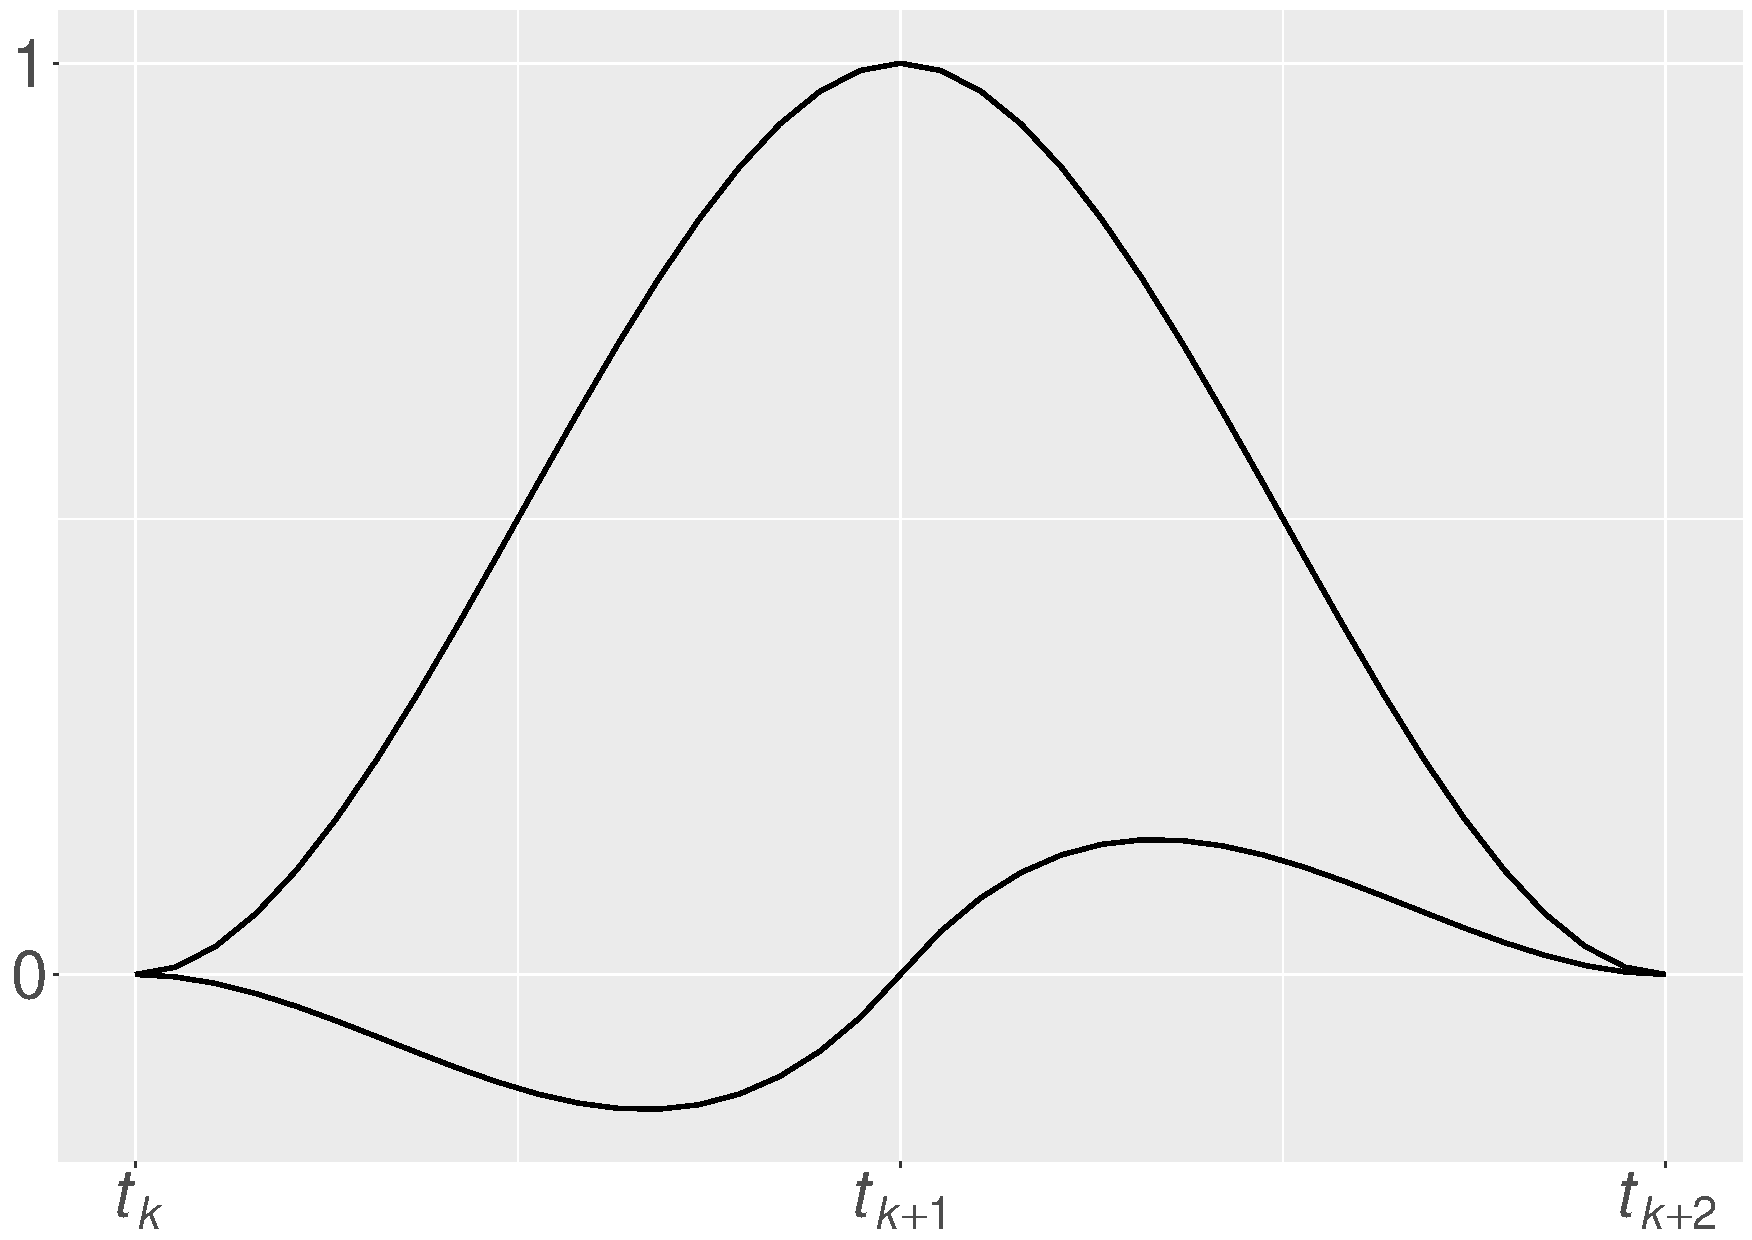
\includegraphics[width=0.6\textwidth, height=4.5cm]{Chapters/02TractorSplineTheory/plot/ggbasistk}
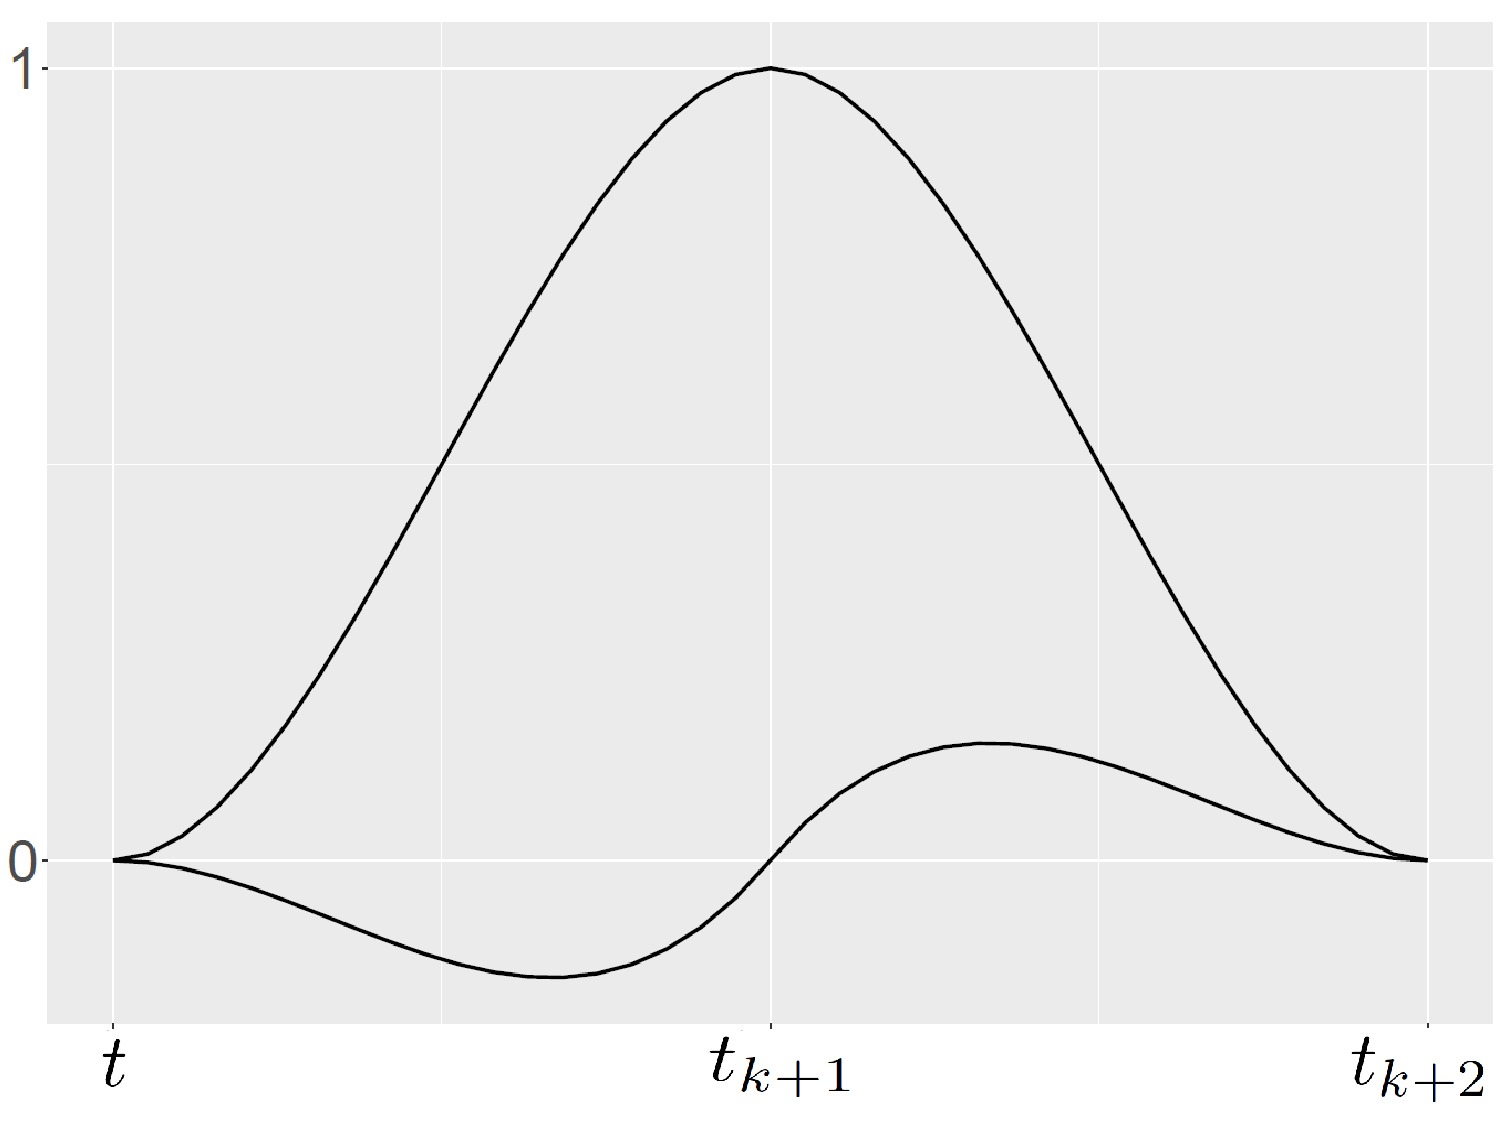
\includegraphics[width=0.6\textwidth, height=5cm]{Chapters/02TractorSplineTheory/plot/pptbasisplot}
%\small 
\caption{The two basis functions $N_{2k+1}$ and $N_{2k+2}$ on an arbitrary interval $[t_k, t_{k+2})$. It is apparently that these basis functions are continuous on this interval and have continuous first derivatives.}
\label{basisfigure}
\end{figure}


From the definition of basis functions, it can be seen that at a joint knot of two neighbor intervals, Hermite spline basis share the same $y_i$ and $v_i$. With this property, we construct Tractor Spline basis functions. There are 2 parameters on each joint knots and 4 on the start and end knots. Then the degrees of freedom for parameters is $2n-4+4=2n$. However $2(n-2)$ constraints are added on the joint knots, on which the spline have continuous first and second derivatives. Additional two constraints are added to the starting and ending knots to keep their first derivatives continuous. Then the degrees of freedom for parameters is 2. 


\subsection{Solution to The Objective Function}

Basis functions have been defined in the previous subsection, therefore the Tractor Spline $f(t)$ on $[a,b]$, where $a \leq t_1 < t_2< \cdots < t_{n-1}<t_n \leq b$, can be found by minimizing  objective function (\ref{tractorsplineObjective}), which reduces to
\begin{equation}\label{tractormse}
\text{MSE}(\theta, \lambda,\gamma) = (\mathbf{y}-\mathbf{B}\theta)^\top (\mathbf{y}-\mathbf{B}\theta) +\gamma (\mathbf{v}-\mathbf{C}\theta)^\top (\mathbf{v}-\mathbf{C}\theta)+n \theta^\top\mathbf{\Omega}_{\lambda}\theta,
\end{equation}
where $\{\mathbf{B}\}_{ij} = N_j(t_i)$ , $\{\mathbf{C}\}_{ij} = N'_j(t_i)$ and $\{\Omega_{2n}^{(k)} \}_{jk}=\int_{t_k}^{t_{k+1}}\lambda_k N''_j(t)N''_k(t)dt$. After substituting the series observation $t_1, \ldots, t_n$ into basis functions, we get $N_1(t_1)=1, N_1(t_2)=0, \ldots, N_{2k-1}(t_{k})=1, N_{2k}(t_{k})=0, \ldots, N_{2n-1}(t_n)=1, N_{2n}(t_n)=0$; and into first derivative of basis functions, we get $N'_1(t_1)=0, N_1'(t_2)=1, \ldots, N_{2k-1}'(t_{k})=0, N_{2k}'(t_{k})=1, \ldots, N_{2n-1}'(t_n)=0, N_{2n}'(t_n)=1$. That means the matrices $\mathbf{B}$ and $\mathbf{C}$ in MSE equation (\ref{tractormse}) are $n \times 2n$ dimensional and the elements are
\begin{align}
\mathbf{B}&=\{B\}_{ij}=\begin{cases}
1, & j=2i-1\\
0, & \mbox{otherwise}
\end{cases}\\
\mathbf{C}&=\{C\}_{ij}=\begin{cases}
1, & j=2i\\
0, & \mbox{otherwise}
\end{cases}
\end{align}
where $i=1, \ldots, n$.  The $k$-th $\Omega_{\lambda_k}^{(k)}$ is a $2n \times 2n$ matrix and its details is in appendix. Then the penalty term is
\begin{equation}
\mathbf{\Omega}_\lambda=\sum_{k=1}^{n-1}\Omega_{\lambda_k}^{(k)},
\end{equation}
which is a bandwidth four matrix.


The solution to (\ref{tractormse}) is easily seen to be
\begin{equation}\label{thetahat}
\hat{\theta}=(\mathbf{B}^\top\mathbf{B}+\gamma\mathbf{C}^\top\mathbf{C}+n\mathbf{\Omega}_{\lambda})^{-1}(\mathbf{B}^\top\mathbf{y}+\gamma\mathbf{C}^\top\mathbf{v})
\end{equation}
a generalized ridge regression. Then the fitted smoothing spline is given by
\begin{equation}
\hat{f}(t)=\sum_{i=1}^{2n}N_i(t)\hat{\theta}_i
\end{equation}

A smoothing spline with parameters $\lambda(t)$ and $\gamma$ is an example of a linear smoother \cite{esl2009}. This is because the estimated parameters in equation (\ref{thetahat}) are a linear combination of $y_i$ and $v_i$. Denote by $\hat{\mathbf{f}}$ and $\hat{\mathbf{f}'}$ the $2n$ vector of fitted values $\hat{f}(t_i)$ and $\hat{f'}(t_i)$ at the training points $t_i$. Then
\begin{equation}
\begin{split}
\hat{\mathbf{f}} =\mathbf{B}(\mathbf{B}^\top\mathbf{B}+\gamma\mathbf{C}^\top\mathbf{C}+n\mathbf{\Omega}_{\lambda})^{-1}(\mathbf{B}^\top\mathbf{y}+\gamma\mathbf{C}^\top\mathbf{v})\\
\triangleq \mathbf{S}_{\lambda,\gamma}\mathbf{y}+\gamma\mathbf{T}_{\lambda,\gamma}\mathbf{v} 
\end{split}
\end{equation}
\begin{equation}
\begin{split}
\hat{\mathbf{f}'}
=\mathbf{C}(\mathbf{B}^\top\mathbf{B}+\gamma\mathbf{C}^\top\mathbf{C}+n\mathbf{\Omega}_{\lambda})^{-1}(\mathbf{B}^\top\mathbf{y}+\gamma\mathbf{C}^\top\mathbf{v})\\
\triangleq\mathbf{U}_{\lambda,\gamma}\mathbf{y}+\gamma\mathbf{V}_{\lambda,\gamma}\mathbf{v}
\end{split}
\end{equation}
The fitted $\hat{\mathbf{f}}$ and $\hat{\mathbf{f}'}$ are linear in $\mathbf{y}$ and $\mathbf{v}$, and the finite linear operators $\mathbf{S}_{\lambda,\gamma}, \mathbf{T}_{\lambda,\gamma}, \mathbf{U}_{\lambda,\gamma}$ and $\mathbf{V}_{\lambda,\gamma}$ are known as the smoother matrices. One consequence of this linearity is that the recipe for producing $\hat{\mathbf{f}}$ and $\hat{\mathbf{f}'}$ from $\mathbf{y}$ and $\mathbf{v}$, do not depend on $\mathbf{y}$ and $\mathbf{v}$ themselves; $\mathbf{S}_{\lambda,\gamma}, \mathbf{T}_{\lambda,\gamma}, \mathbf{U}_{\lambda,\gamma}$ and $\mathbf{V}_{\lambda,\gamma}$ depend only on $t_i,\lambda(t)$ and $\gamma$.

Suppose in a traditional least squares fitting, $\mathbf{B}_\xi$ is $N \times M$ matrix of $M$ cubic-spline basis functions evaluated at the $N$ training points $x_i$, with knot sequence $\xi$ and $M \ll N$. Then the vector of fitted spline values is given by
\begin{align}\label{fhy}
\hat{\mathbf{f}}=\mathbf{B}_\xi(\mathbf{B}^\top_\xi\mathbf{B}_\xi)^{-1}\mathbf{B}_\xi\mathbf{y}=\mathbf{H}_\xi\mathbf{y}
\end{align}
Here the linear operator $\mathbf{H}_\xi$ is a symmetric, positive semidefinite matrices, and $\mathbf{H}_\xi\mathbf{H}_\xi=\mathbf{H}_\xi$ (idempotent) \cite{esl2009}. In our case, it is easily seen that $\mathbf{S}_{\lambda,\gamma}, \mathbf{T}_{\lambda,\gamma}, \mathbf{U}_{\lambda,\gamma}$ and $\mathbf{V}_{\lambda,\gamma}$ are symmetric, positive semidefinite matrices as well. Additionally, by Cholesky decomposition
\begin{equation}
(\mathbf{B}^\top\mathbf{B}+\gamma\mathbf{C}^\top\mathbf{C}+n\mathbf{\Omega}_{\lambda})^{-1}=\mathbf{R}\mathbf{R}^\top,
\end{equation}
it is easily to prove that $\mathbf{T}_{\lambda,\gamma}=\mathbf{B}\mathbf{R}\mathbf{R}^\top\mathbf{C}^\top$ and $\mathbf{U}_{\lambda,\gamma}=\mathbf{C}\mathbf{R}\mathbf{R}^\top\mathbf{B}^\top$, then we will have 
 $\mathbf{T}_{\lambda,\gamma}= \mathbf{U}_{\lambda,\gamma}^\top$. When $\lambda=\gamma=0$, the matrix $\mathbf{S}_{\lambda_0,\gamma_0}=\mathbf{B}(\mathbf{B}^\top\mathbf{B})^{-1}\mathbf{B}^\top$ is idempotent.  

For sufficient cases of $\lambda(t)$ and $\gamma$, Tractor Spline has the following property:
\begin{itemize}
\item if $\lambda(t)$ is a piecewise constant and $\gamma \neq 0$, then $f$ and $f'$ are continuous, $f''$ is piecewise linear but not continuous at knots;
\item if $\lambda(t)$ is a piecewise constant and $\gamma = 0$, the same as above;
\item if $\lambda(t)=\lambda $ is a constant and $\gamma \neq 0$, the same as above;
\item if $\lambda(t)=\lambda $ is a constant and $\gamma = 0$, then $f$, $f'$ are continuous, $f''$ is piecewise linear and continuous at knots.
\end{itemize}

%Then we take some sample knots $\mathbf{y}^{(new)}$ with the same size of $\mathbf{y}$ from $\hat{\mathbf{f}}$ and reconstruct the spline function. It is easily seen that
% \begin{equation}
%\hat{\mathbf{f}}^{(new)} = \mathbf{S}_{\lambda_0,\gamma_0}\mathbf{y}^{(new)}=\mathbf{S}_{\lambda_0,\gamma_0}\mathbf{S}_{\lambda_0,\gamma_0}\mathbf{y}=(\mathbf{B}(\mathbf{B}^\top\mathbf{B})^{-1}\mathbf{B}^\top)(\mathbf{B}(\mathbf{B}^\top\mathbf{B})^{-1}\mathbf{B}^\top)=\mathbf{S}_{\lambda_0,\gamma_0}\mathbf{y},
 %\end{equation}
 %which returns the same reconstruction. So $\hat{\mathbf{f}}$ is generated and only affected by $\mathbf{y}$. And the same as $\hat{\mathbf{f}'}$, because
%\begin{equation}
%\hat{\mathbf{f}'}^{(new)}=\mathbf{U}_{\lambda_0,\gamma_0}\mathbf{y}^{(new)}=\mathbf{U}_{\lambda_0,\gamma_0}\mathbf{S}_{\lambda_0,\gamma_0}\mathbf{y}=(\mathbf{C}\mathbf{B} (\mathbf{B}^\top\mathbf{B})^{-1}\mathbf{B}^\top)(\mathbf{B}(\mathbf{B}^\top\mathbf{B})^{-1}\mathbf{B}^\top)\mathbf{y}=\mathbf{U}_{\lambda_0,\gamma_0}\mathbf{y}.
%\end{equation}
 %That means no matter how many times we reconstruct Tractor Spline, once the matrices are fixed and observed knots are given, it will always return the same results when $\lambda=\gamma=0$.

%\begin{theorem}
%For $n\geq 2$, the objective function $J[f]$ in equation (\ref{tractorsplineObjective}) is minimized by a Tractor Spline.
%\end{theorem}



\subsection{Adjusted Penalty Term and Parameter Function}

To get the reconstructed trajectory in a multi-dimensional space, one can use the Tractor Spline to find the trajectory in each dimension separately  and then combine them together for a higher dimension, such as 2D and 3D. Typically, the data are not regularly sampled in time. Due to the property of Hermite spline, the combination of a multi-dimensional reconstruction for irregular time difference dataset will bring some issues.  Image the situation in which a vehicle is moving along the $x$-axis, but stays unchanged on its $y$ position. By fitting $\mathbf{x}$ and $\mathbf{u}$, the Tractor Spline $f_x(t)$ will give us a best fit which returns smallest errors to the objective function. While with the same parameter $\lambda(t)$ and $\gamma$, $f_y(t)$ returns a cubic curve, where it should give us a straight line as we expected. Moreover, in some circumstances, with time increasing $\mathbf{f}$ and $\mathbf{f}'$ remain the same, or change slightly. In this situation, the Hermite spline will return wiggles in each dimension and curves in combined two dimensions. 

To get a reliable reconstruction, we introduce an adjusted penalty term $\frac{(\Delta t_i)^\alpha}{(\Delta d_i)^\beta}$, where $\alpha \ge 0$ and $\beta \ge 0$, to the penalty function $\lambda(t)$, in which the Tractor Spline is penalized by its real difference of $\Delta d_i$ and $\Delta t_i$ for each interval $[t_i, t_{i+1}]$. With this term, when either $\mathbf{u}$ for $x$ or $\mathbf{v}$ for $y$ goes down or equals to 0, it will make sure that the penalty function will be large enough and returns a straight line rather than a curve on this domain. Because of the unit of the penalty term is $m^2/t^3$, to keep the same scale, $\alpha$ and $\beta$ in the adjusted penalty term are chosen as $3$ and $2$ respectively. From the physical point of view, the term is the reciprocal of the product of velocity and acceleration. Either velocity or acceleration goes to zero, the moving object should either stop, which returns a straight line along time on $x$ or $y$ axises and a dot on higher dimension, or keep moving with the same speed, which returns a linear  instead of a curve path. 

Consequently, the final form of the penalty function is 
\begin{equation}\label{adjustedpenalty}
\lambda(t)=\frac{(\Delta t_i)^3}{(\Delta d_i)^2}\lambda,
\end{equation}
where  $t_i\leq t < t_{i+1}$. Eventually, in objective function, there is one parameter $\lambda$ controlling the curvature of Tractor Spline on different domains, and another one $\gamma$ controlling the residuals of velocity. 




\section{Parameter Selection and Cross Validation}

The problem of choosing the smoothing parameter is ubiquitous in curve estimation, and there are two different philosophical approaches to this question. The first one is to regard the free choice of smoothing parameter as an advantageous feature of the procedure. The other one is to find the parameter automatically by the data \cite{green1993nonparametric}. We prefer the latter one, use data to train our model and find the best parameters. The most well known method is cross-validation.


Assuming that the random errors have zero mean, the true regression curve $f(t)$ has the property that, if an observation $y$ is taken at a point $t$, the value $f(t)$ is the best predictor of $y$ in terms of returning a small value of $(y-f(t))^2$. 

Now we focus on an observation $y_i$ at point $t_i$ as being a new observation by omitting it from the set of data, which are used to estimate $\hat{f}$. Denote by $\hat{f}^{(-i)}(t,\lambda)$ the estimated function from the remaining data, where $\lambda$ is the smoothing parameter. Then $\hat{f}^{(-i)}(t,\lambda)$ minimizes 
\begin{align}\label{originalcv}
\frac{1}{n}\sum_{j \neq i}(y_j-f(t_j))^2+\lambda \int f''^2dt
\end{align}
 and $\lambda$ can be quantified by cross-validation score function
\begin{align}
\mbox{CV}(\lambda)=\frac{1}{n}\sum_{i=1}^{n}\left(  y_i-\hat{f}^{(-i)}(t_i,\lambda)\right) ^2.
\end{align}
The basis idea of cross-validation is to choose the value of $\lambda$ that minimizes $\mbox{CV}(\lambda)$. 

An efficient way to calculate cross validation score is given by \cite{green1993nonparametric}. Through the equation (\ref{fhy}), we know that the value of the smoothing spline $\hat{f}$ depend linearly on the data $y_i$. Define the matrix $A(\lambda)$, which is a map vector of observed values $y_i$ to predicted values $\hat{f}(t_i)$. Then we have
\begin{equation}
\hat{\mathbf{f}}=A(\lambda)\mathbf{y}
\end{equation}
and the following lemma.
\begin{lemma}\label{cvlema}
The cross validation score satisfies
\begin{equation}
\mbox{CV}(\lambda)=\frac{1}{n} \sum_{i=1}^n \left(\frac{y_i-\hat{f}(t_i)}{1-A_{ii}(\lambda)}\right)^2
\end{equation}
where $\hat{f}$ is the spline smoother calculated from the full data set $\{(t_i,y_i)\}$ with smoothing paramter $\lambda$.
\end{lemma}

For a Tractor Spline and its MSE function, there are two parameters need to be estimated $\lambda$ and $\gamma$. Then the objective function (\ref{originalcv}) becomes
\begin{align}
\frac{1}{n}\sum_{j \neq i}\lVert y_j-f(t_j) \rVert_2^2+\frac{\gamma}{n}\sum_{j \neq i} \lVert v_j-f'(t_j) \rVert_2^2+ \int \lambda(t) \lVert f''\rVert_2^2dt,
\end{align}
and the cross-validation score function is
\begin{align}
\mbox{CV}(\lambda,\gamma)=\frac{1}{n}\sum_{i=1}^{n}\left( y_i-\hat{f}^{(-i)}(t_i,\lambda,\gamma) \right) ^2.
\end{align}

For a Tractor Spline, the parameter $\hat{\theta}=(B^\top B+\gamma C^\top C+n\Omega_\lambda)^{-1}(B^\top\mathbf{y}+\gamma C^\top\mathbf{v})$ gives us
\begin{equation}
\begin{split}
 \hat{\mathbf{f}}&=B\hat{\theta}=B(B^\top B+\gamma C^\top C+n\Omega_\lambda)^{-1}B^\top\mathbf{y}+B(B^\top B+\gamma C^\top C+n\Omega_\lambda)^{-1}C^\top\mathbf{v}\\&=S\mathbf{y}+\gamma T\mathbf{v},
 \end{split}
 \end{equation}
 \begin{equation}
 \begin{split}
\hat{\mathbf{f}}'&=C\hat{\theta}=C(B^\top B+\gamma C^\top C+n\Omega_\lambda)^{-1}B^\top\mathbf{y}+C(B^\top B+\gamma C^\top C+n\Omega_\lambda)^{-1}C^\top\mathbf{v}\\&=U\mathbf{y}+\gamma V\mathbf{v}.
 \end{split}
\end{equation}
From lemma \ref{cvlema}, we can prove the following theorem.
\begin{theorem}\label{cvscore}
The cross validation score of a Tractor Spline satisfies
\begin{equation}\label{tractorcv}
\mbox{CV}(\lambda,\gamma)=\frac{1}{n}\sum_{i=1}^{n} \left( \frac{\hat{f}(t_i)-y_i+\gamma \frac{T_{ii}}{1-\gamma V_{ii}}(\hat{f}'(t_i)-v_i)}{1-S_{ii}-\gamma\frac{T_{ii}}{1-\gamma V_{ii}}U_{ii}} \right)^2
\end{equation}
where $\hat{f}$ is the Tractor Spline smoother calculated from the full data set $\{(t_i,y_i,v_i)\}$ with smoothing parameter $\lambda$ and $\gamma$.
\end{theorem}

The proof of Theorem \ref{cvscore} follows immediately from a lemma, and gives an expression for the deleted residuals $y_i-\hat{f}^{(-i)}(t_i)$ and $v_i-\hat{f}'^{(-i)}(t_i)$ in terms of $y_i-\hat{f}(t_i)$ and $v_i-\hat{f}'(t_i)$ respectively. 

\begin{lemma} \label{cvlemma}
For fixed $\lambda,\gamma$ and $i$, denote $\mathbf{f}^{(-i)}$ by the vector with components $f_j^{(-i)}=\hat{f}^{(-i)}(t_j,\lambda,\gamma)$,  $\mathbf{f}'^{(-i)}$ by the vector with components $f_j'^{(-i)}=\hat{f}'^{(-i)}(t_j,\lambda,\gamma)$, and define vectors $\mathbf{y}^*$ and $\mathbf{v}^*$ by 
\begin{align}
\begin{cases}
y_j^*=y_j &j \neq i\\
y_i^*=\hat{f}^{(-i)}(t_i) &\mbox{otherwise}
\end{cases},\\
\begin{cases}
v_j^*=v_j &j \neq i\\
v_i^*=\hat{f}'^{(-i)}(t_i) &\mbox{otherwise}
\end{cases}.
\end{align}
Then
\begin{align}
\mathbf{\hat{f}}^{(-i)}&=S\mathbf{y}^*+\gamma T\mathbf{v}^*\\
\mathbf{\hat{f}}'^{(-i)}&=U\mathbf{y}^*+\gamma V\mathbf{v}^*
\end{align}
\end{lemma}


\section{Simulation Study} %and Error Analysis}


\subsection{Numerical Examples}

In this section, we examine the visual quality of the proposed method with four functions: \textit{Blocks}, \textit{Bumps}, \textit{HeaviSine} and \textit{Doppler}, which have been used in \cite{donoho1994ideal}, \cite{donoho1995adapting} and \cite{abramovich1998wavelet} because of their caricature features in imaging, spectroscopy and other scientific signal processing. However it is unfair for Tractor Spline fitting "jump" position in \textit{Blocks} and \textit{Bumps} function, because it fits position and velocity simultaneously and these points imply infinite first derivative in original functions, which are impossible for vehicles or individuals. In terms of this issue, we treat these functions as velocity, and use noise free points to generate accurate position data, then add noises back to them.

For calculating consideration, we use $n=1024$ \cite{nason2010wavelet}. Because all noises are randomly generated, for convenience of reinitialization and repetition of comparing, we set random seed as 2016. The noises are independent Gaussian distribution $\epsilon \sim N(0,1)$ and signal-to-noise ratio (SNR), which is defined as the ratio of the power of a signal and the power of background noise, is set at 7. These data are treated as velocity (first derivative). By setting initial position $y_0=0$, acceleration $a_0=0$ and using the following formula 
\begin{equation}
y_{i+1}=y_i+(v_i+v_{i+1})\frac{t_{i+1}-ti}{2}
\end{equation}
to calculate position information, we can easily generate simulated data. Then we add some i.i.d. $\epsilon \sim N(0,1)$ with SNR 7 noises on it. For wavelet transform reconstructions, we use the threshold policy of \textit{sure} and \textit{BayesThresh} with levels $j=4, \ldots, 9$, see  \cite{donoho1995adapting} and \cite{abramovich1998wavelet}. A semi-parametric regression model with spatially adaptive penalized splines (P-spline) is added in comparison, see \cite{krivobokova2008fast} \cite{ruppert2003semiparametric}.

For Tractor Spline, we have two parameters $\lambda$ and $\gamma$ to optimize. To evaluate the performance of the velocity term in objective function (\ref{tractorsplineObjective}) and the adjusted penalty term in (\ref{adjustedpenalty}), the parameter $\gamma$ is set as 0 in one reconstruction of Tractor Spline, whose objective function and solution become
\begin{equation}\label{ofgamma0}
J[f]_{\gamma=0}= \frac{1}{n} \sum_{i=1}^{n} (f(t_i)-y_i)^2 +\sum_{i=1}^{n-1} \lambda_i\int_{t_i}^{t_{i+1}} f''(t)^2 dt,
\end{equation}
and
\begin{equation}\label{thetahat0}
\hat{\theta}_{\gamma=0}=(\mathbf{B}^\top\mathbf{B}+n\Omega_{\lambda})^{-1}\mathbf{B}^\top\mathbf{y}
\end{equation}
and the adjusted penalty term in (\ref{adjustedpenalty}) was removed from another reconstruction, noted as "Tractor Spline without APT". Figure (\ref{num1}) to (\ref{num4}) display the original (velocity), generated position, wavelet with two different threshold methods, P-spline and three kinds of Tractor Spline fitted functions. The parameters $\lambda$ and $\gamma$ of a Tractor Spline are automatically selected from formula (\ref{tractorcv}) by $\textit{optim}$ function in $R$ \cite{nelder1965simplex}.


%\begin{figure}
%  \centering
%   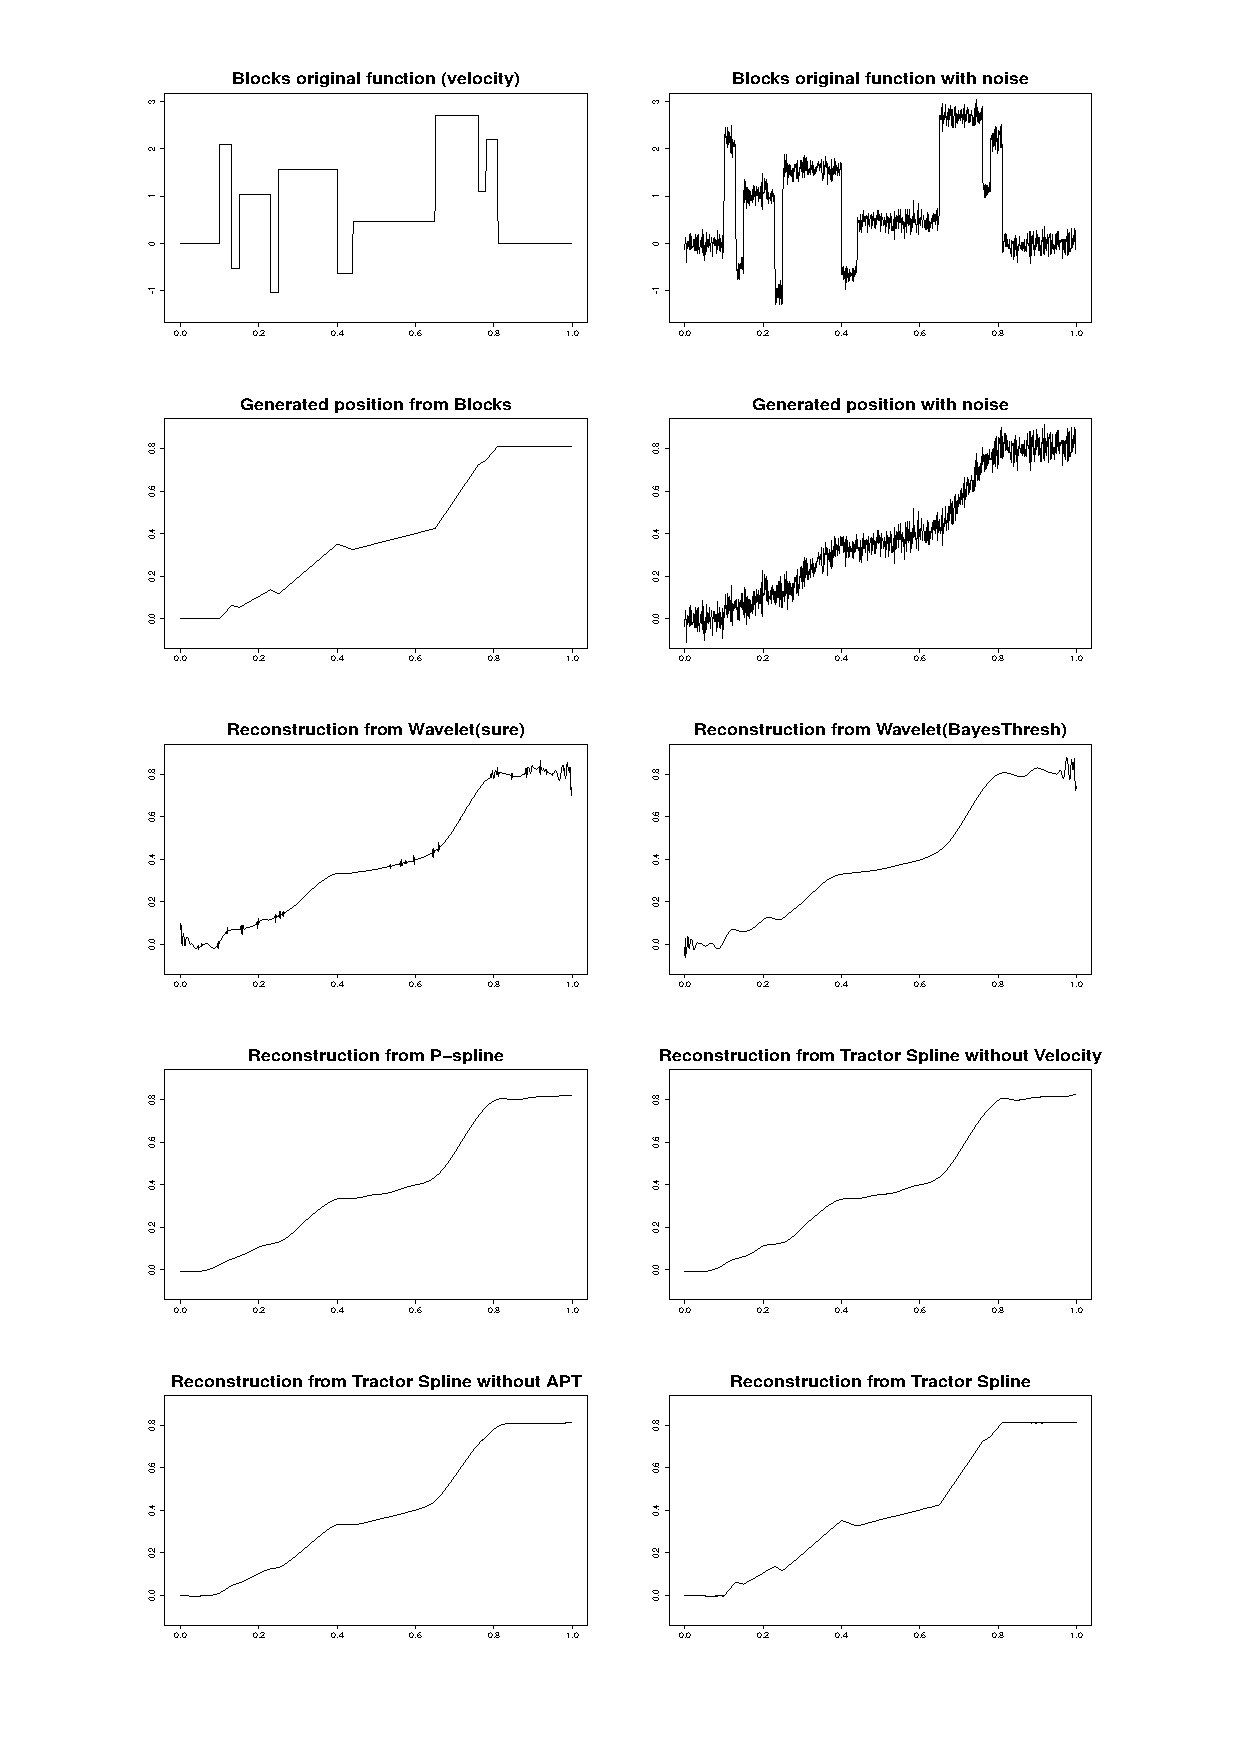
\includegraphics[width=\textwidth,height=14cm]{Chapters/02TractorSplineTheory/plot/blocks10} 
%  \caption{Numerical example: $\textit{Blocks}$. (a) The true velocity function. (b) Velocity with Gaussian noise at SNR=7. (c) Generated position function. (d) Position with Gaussian noise at SNR=7. (e) Reconstruction from Wavelet with sure threshold. (f) Reconstruction from Wavelet with BayesThresh approach. (g) Reconstruction by P-spline. (h) Reconstruction by Tractor Spline setting $\gamma=0$. (i) Reconstruction by Tractor Spline with normal penalty term. (j) Reconstruction by proposed Tractor Spline.}\label{num1}
%\end{figure}

\begin{figure}
    \centering
    \begin{subfigure}{0.45\textwidth}
    \centering
    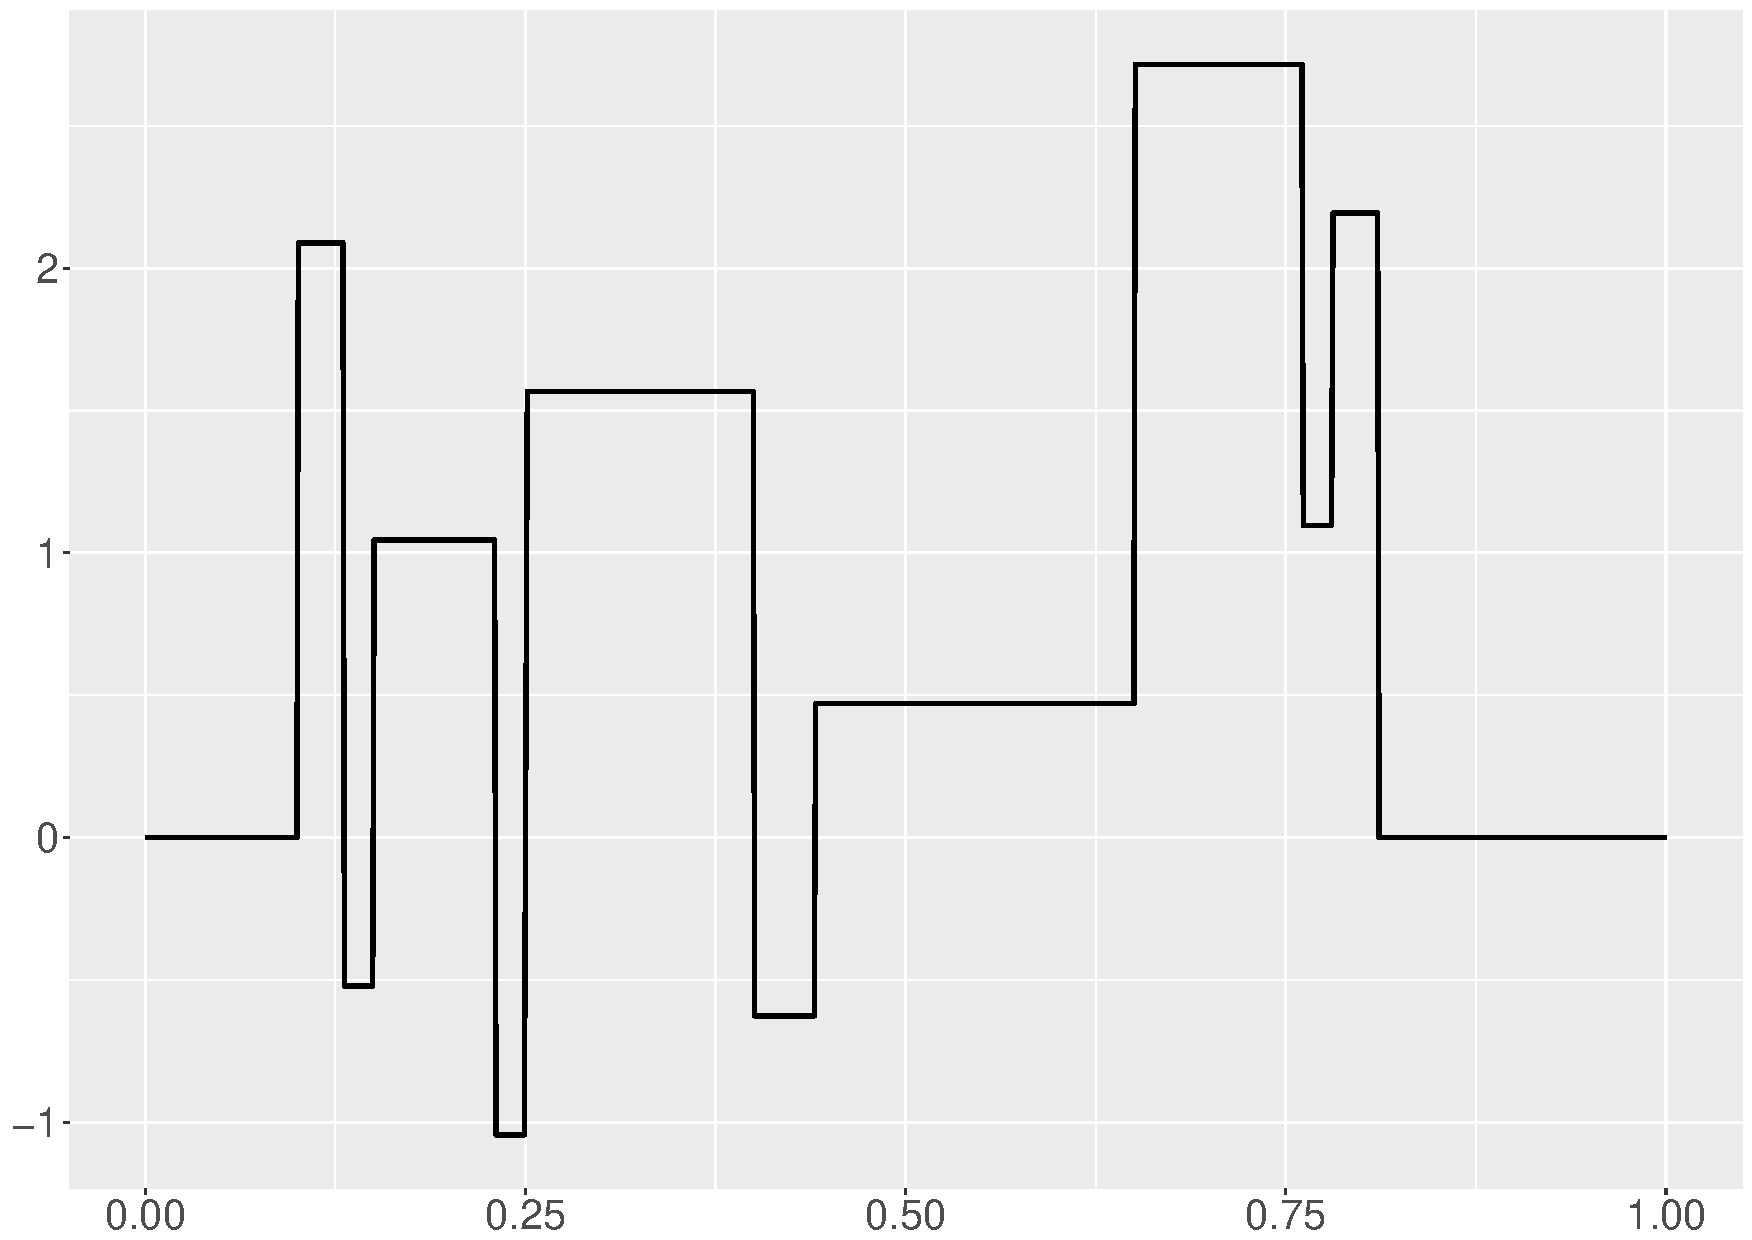
\includegraphics[width=\linewidth,height=0.45\textwidth]{Chapters/02TractorSplineTheory/plot/ggplot/ggBlocks.pdf}
    \caption{The \textit{Blocks} function.}
    \end{subfigure}%
    \begin{subfigure}{0.45\textwidth}
    \centering
    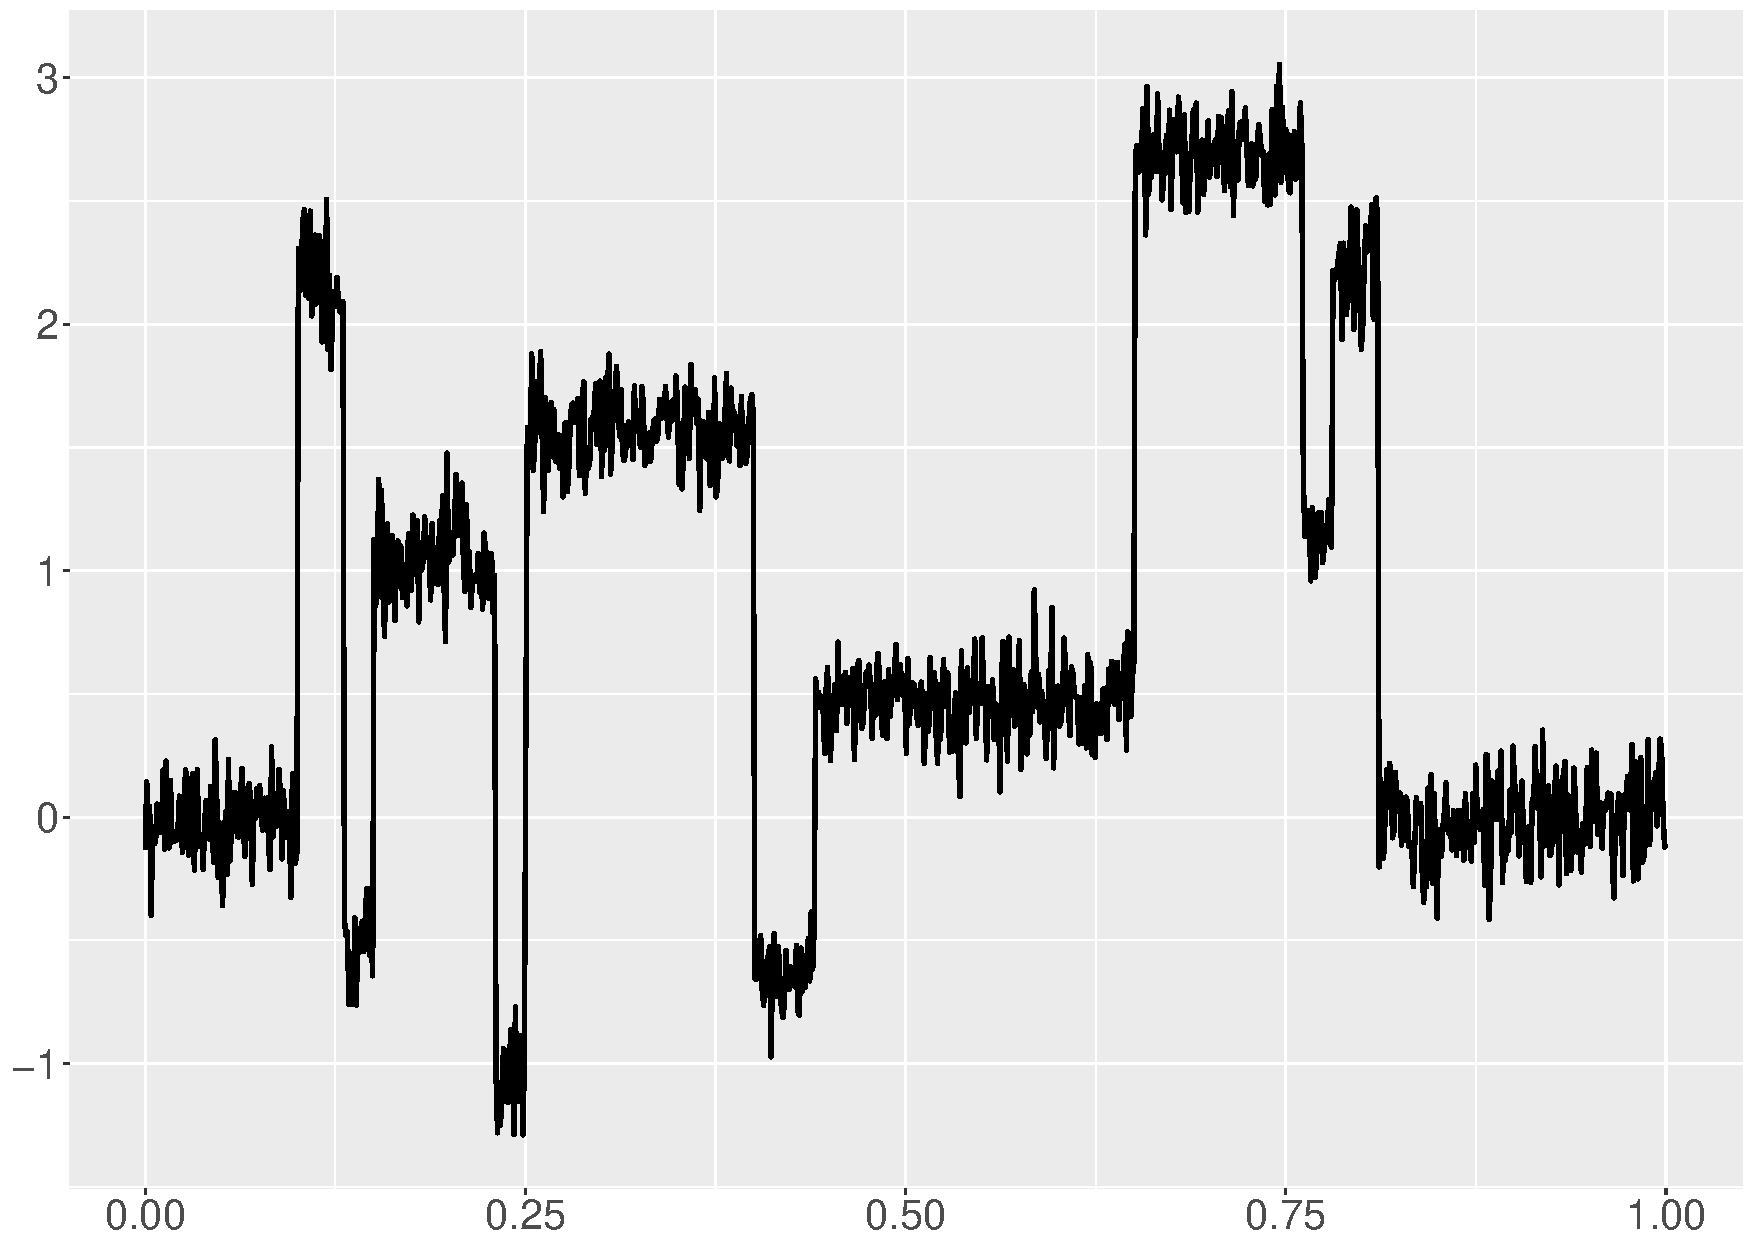
\includegraphics[width=\linewidth,,height=0.45\textwidth]{Chapters/02TractorSplineTheory/plot/ggplot/ggBlocksNoise.pdf}
    \caption{Noisy \textit{Blocks} at \textit{SNR}=7.}
    \end{subfigure}
    \begin{subfigure}{0.45\textwidth}
    \centering
    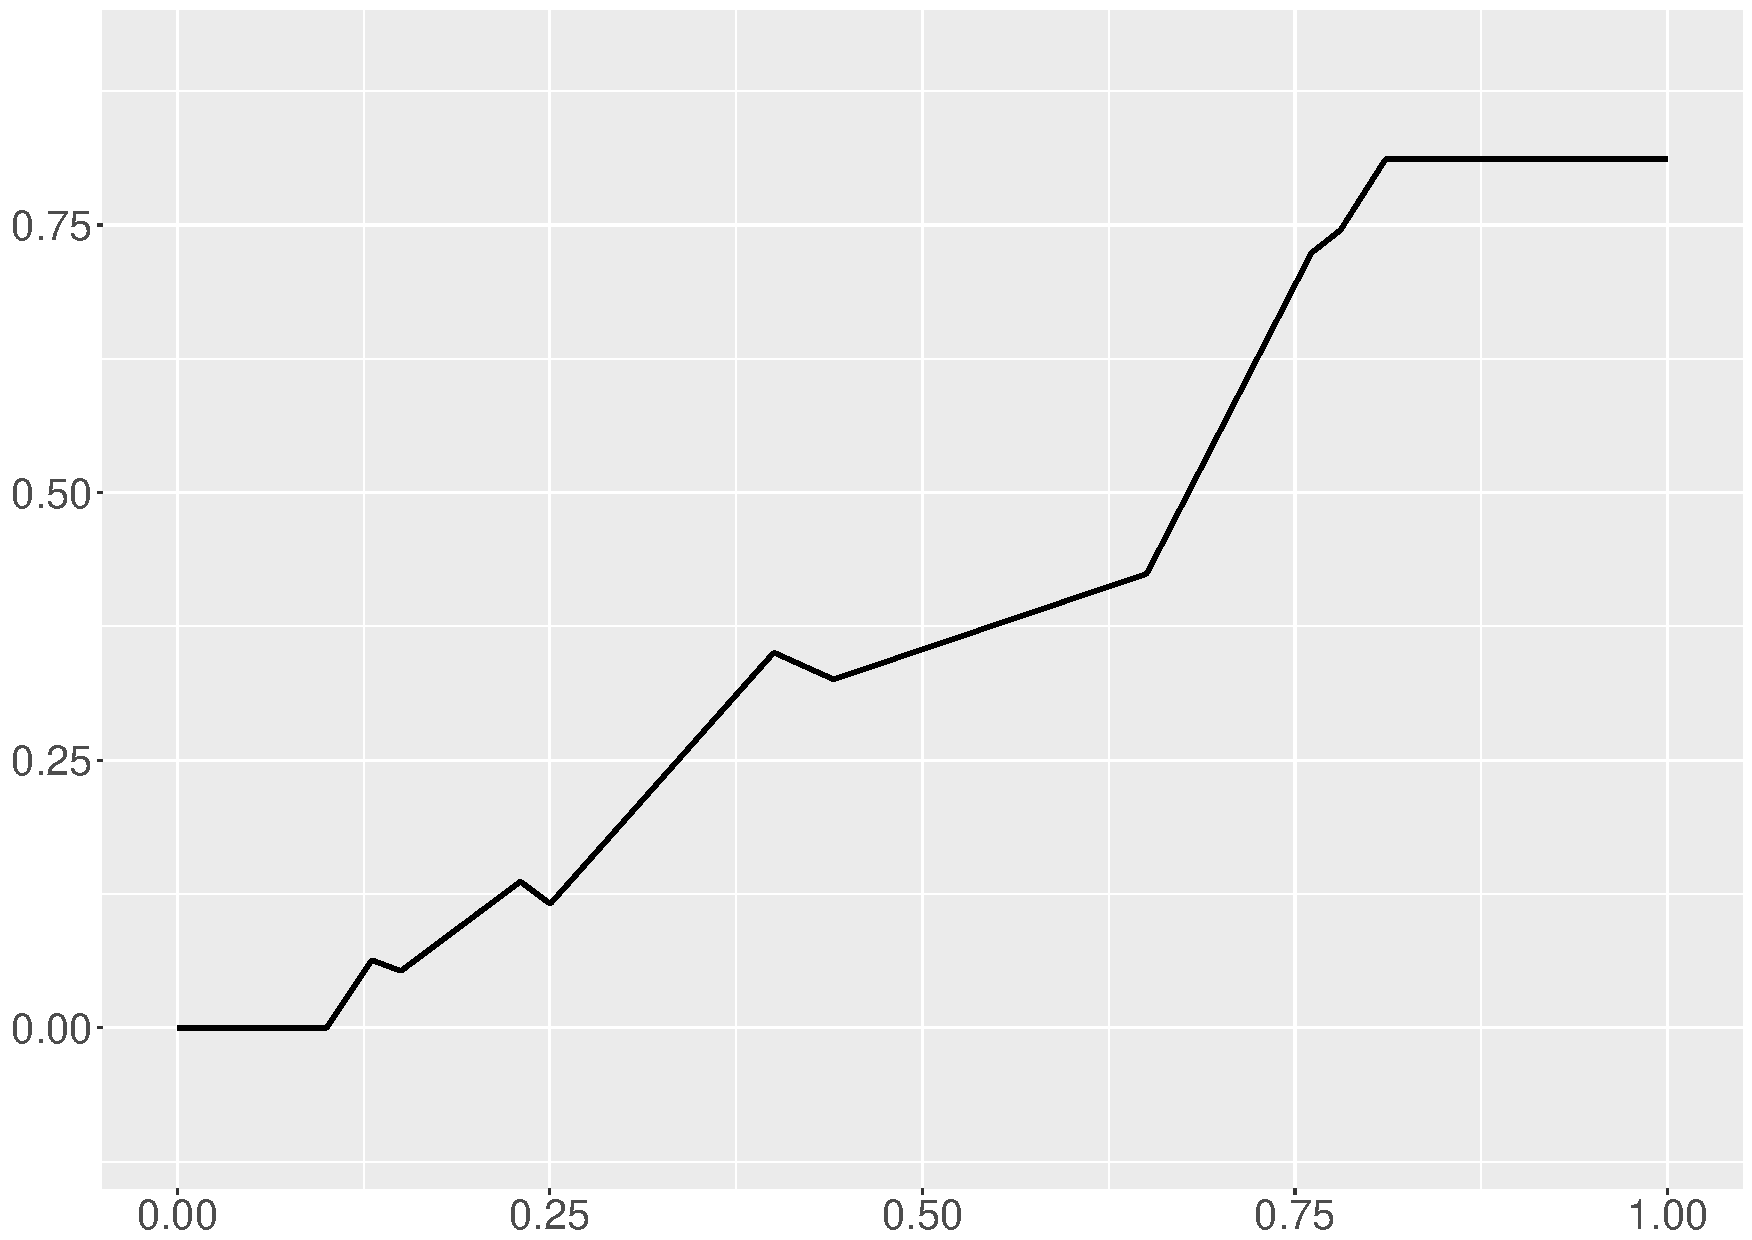
\includegraphics[width=\linewidth,height=0.45\textwidth]{Chapters/02TractorSplineTheory/plot/ggplot/ggBlocksPosition.pdf}
    \caption{Generated positions.}
    \end{subfigure}
    \begin{subfigure}{0.45\textwidth}
    \centering
    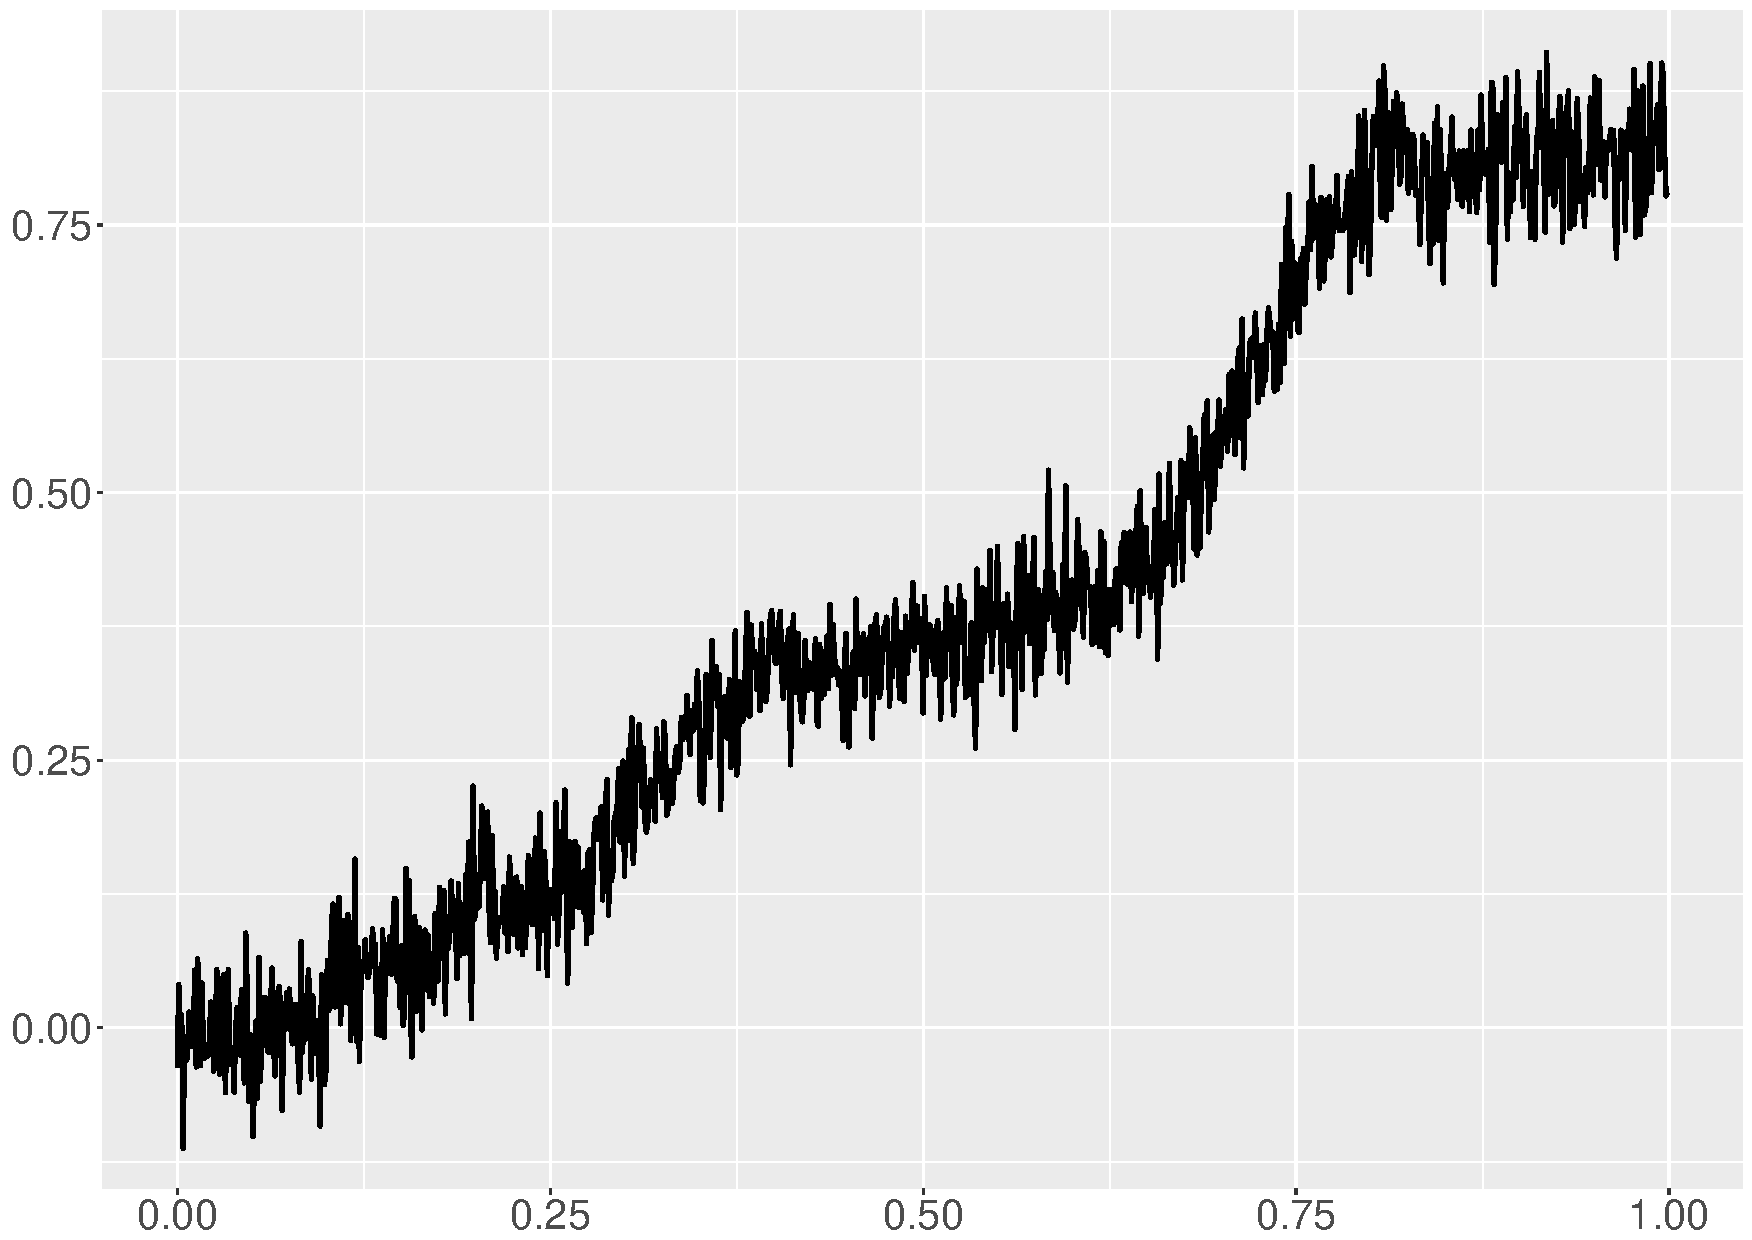
\includegraphics[width=\linewidth,height=0.45\textwidth]{Chapters/02TractorSplineTheory/plot/ggplot/ggBlocksPositionNoise.pdf}
    \caption{Noisy position at \textit{SNR}=7.}
    \end{subfigure}
    \begin{subfigure}{0.45\textwidth}
    \centering
    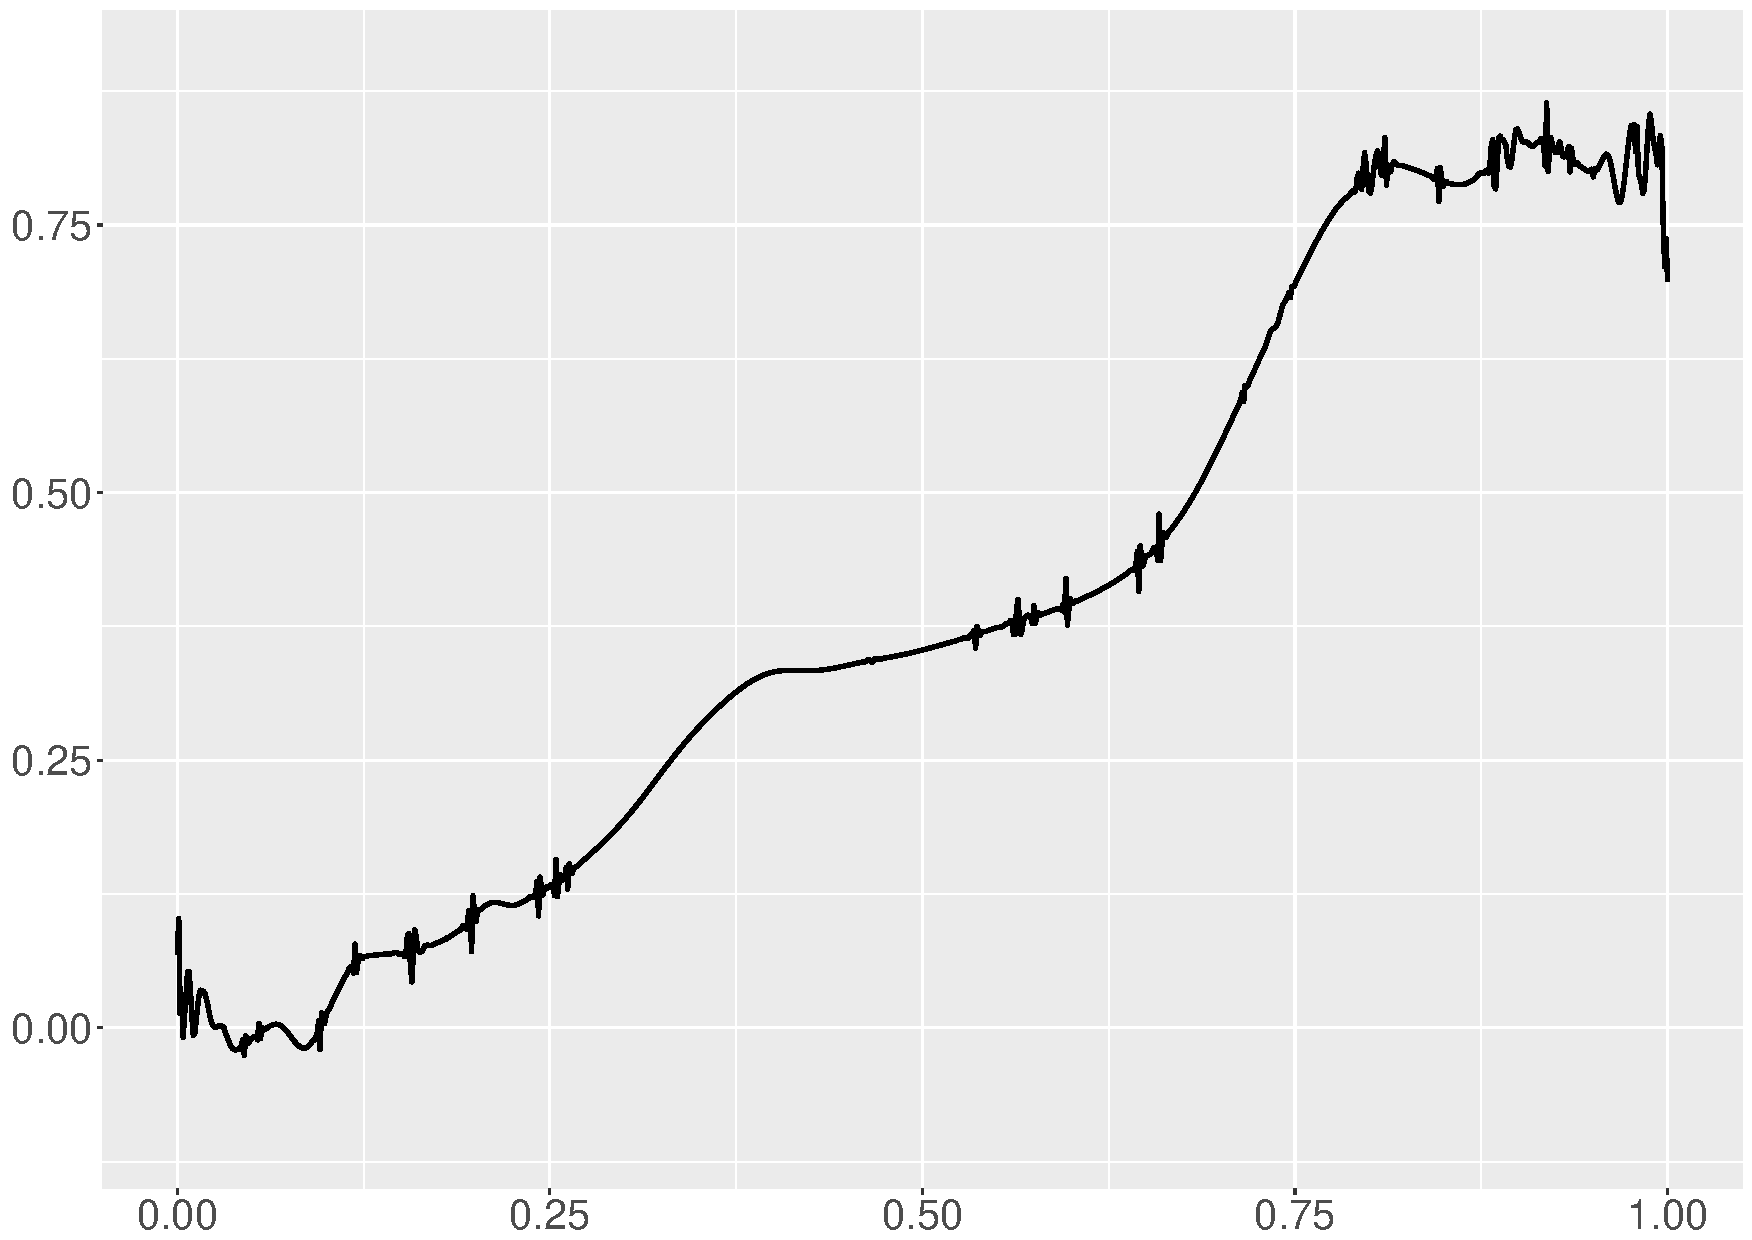
\includegraphics[width=\linewidth,height=0.45\textwidth]{Chapters/02TractorSplineTheory/plot/ggplot/ggBlocksSure.pdf}
    \caption{Reconstruction from Wavelet by sure threshold.}
    \end{subfigure}
    \begin{subfigure}{0.45\textwidth}
    \centering
    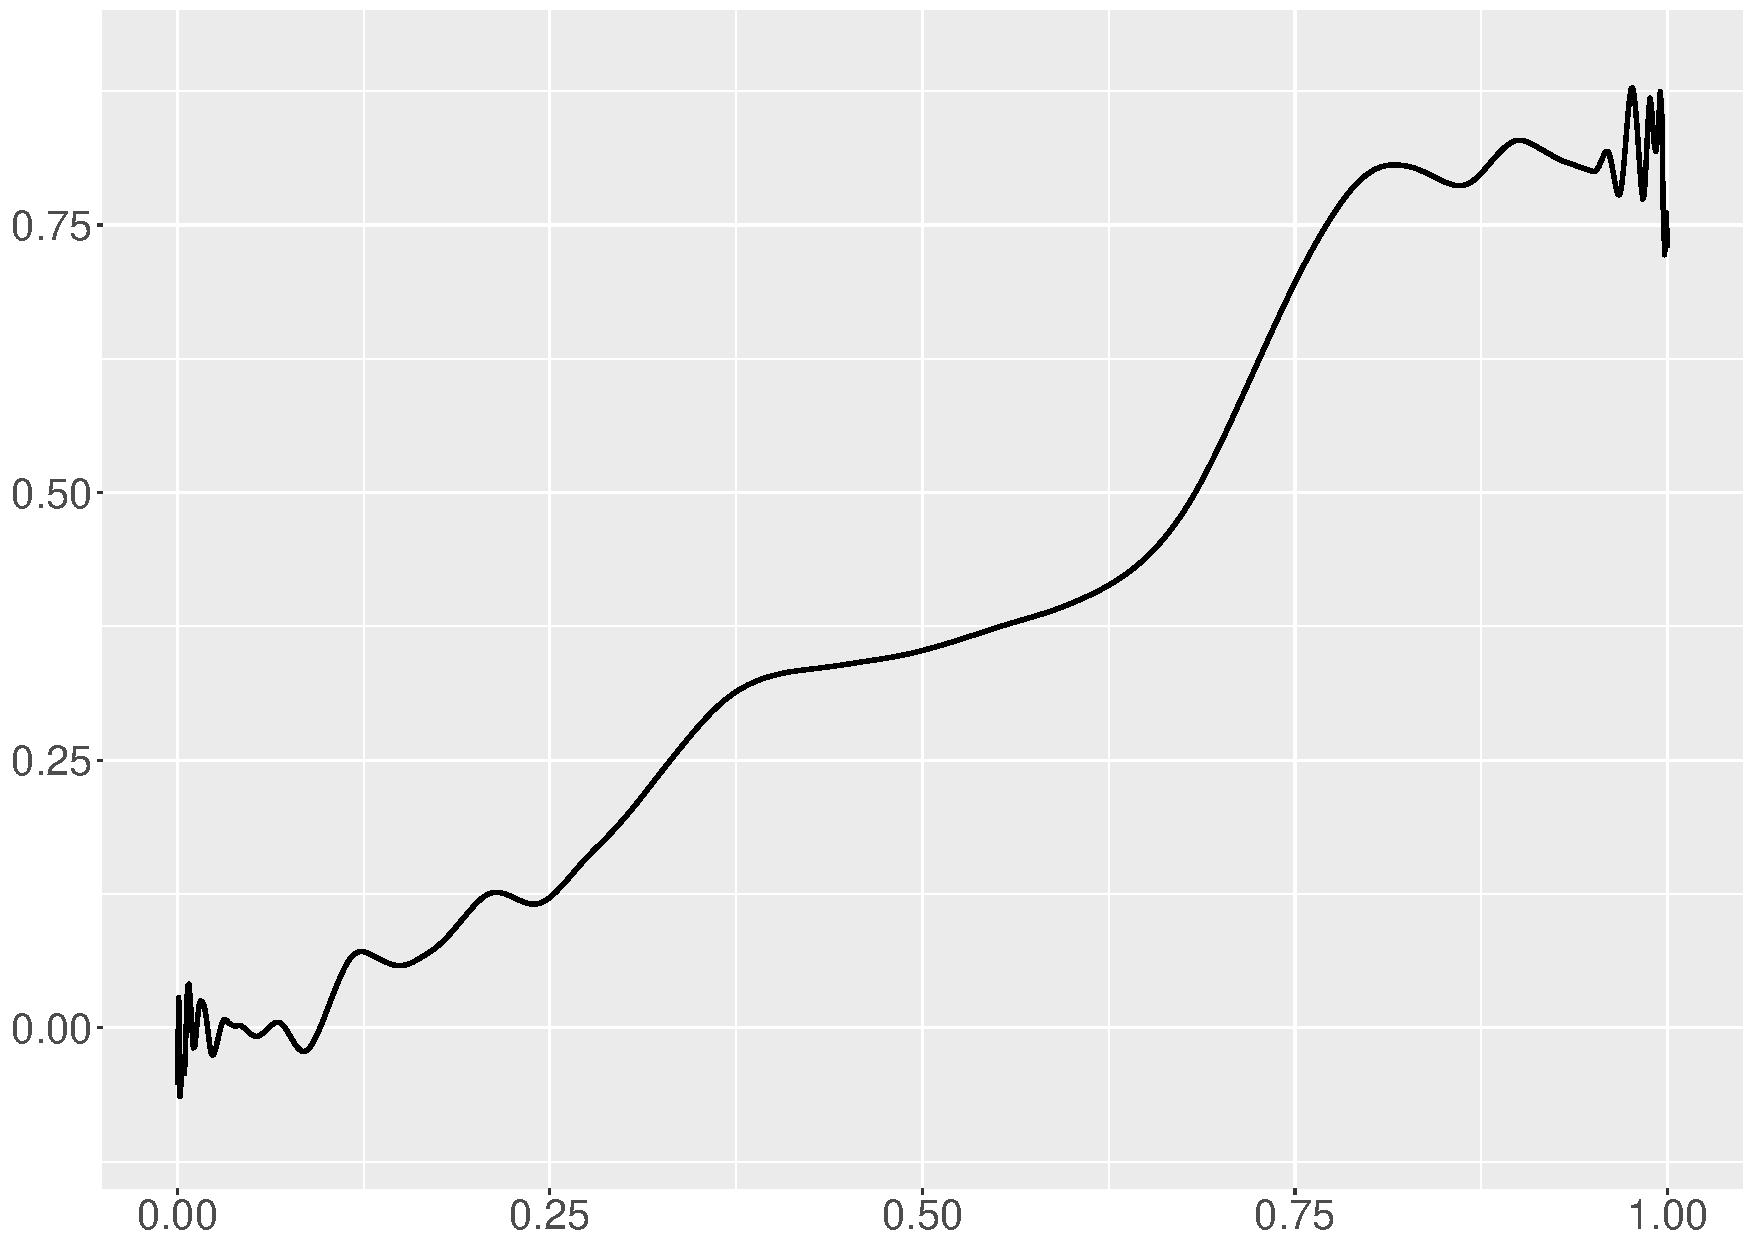
\includegraphics[width=\linewidth,height=0.45\textwidth]{Chapters/02TractorSplineTheory/plot/ggplot/ggBlocksBayes.pdf}
    \caption{Reconstruction from Wavelet by BayesThresh approach.}
    \end{subfigure}
    \begin{subfigure}{0.45\textwidth}
    \centering
    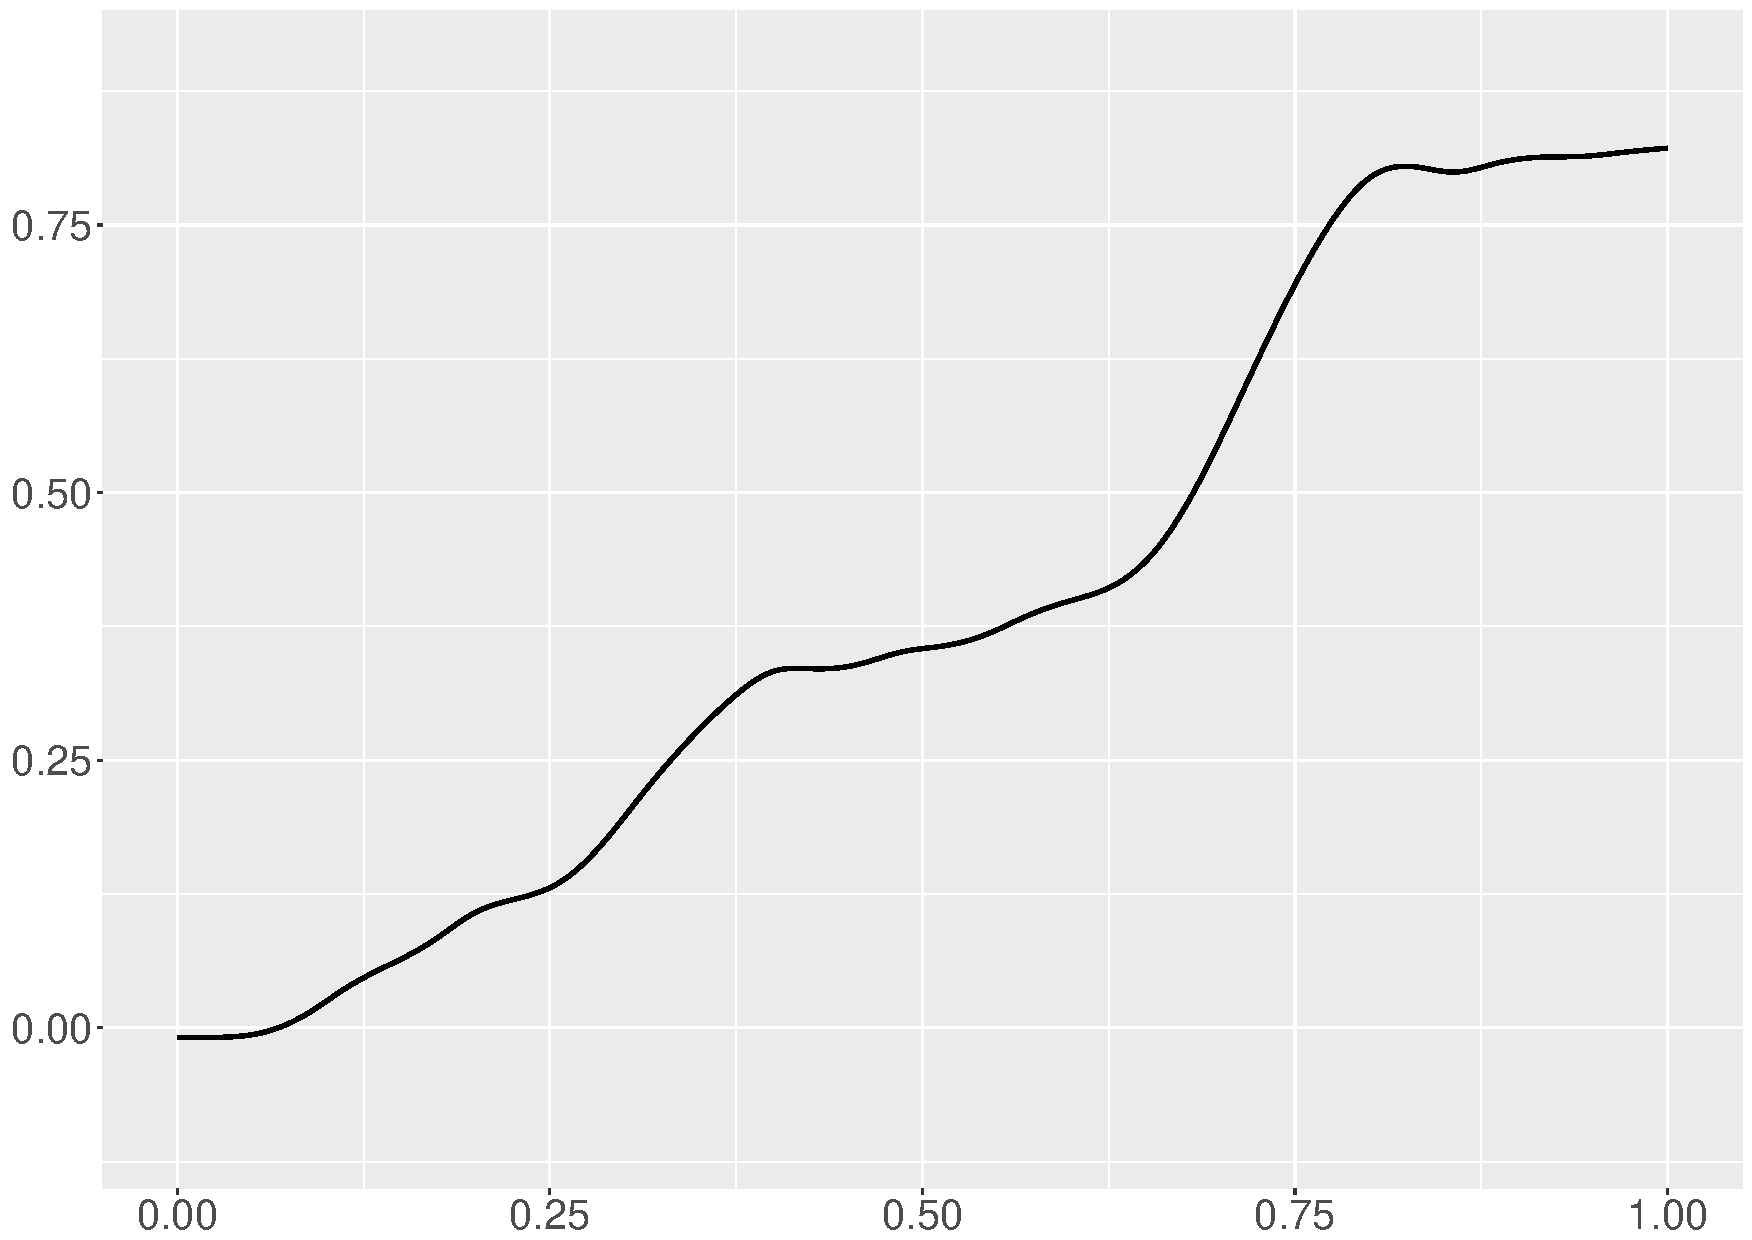
\includegraphics[width=\linewidth,height=0.45\textwidth]{Chapters/02TractorSplineTheory/plot/ggplot/ggBlocksPSpline.pdf}
    \caption{Reconstruction by P-spline. \\\mbox{  } }
    \end{subfigure}
    \begin{subfigure}{0.45\textwidth}
    \centering
    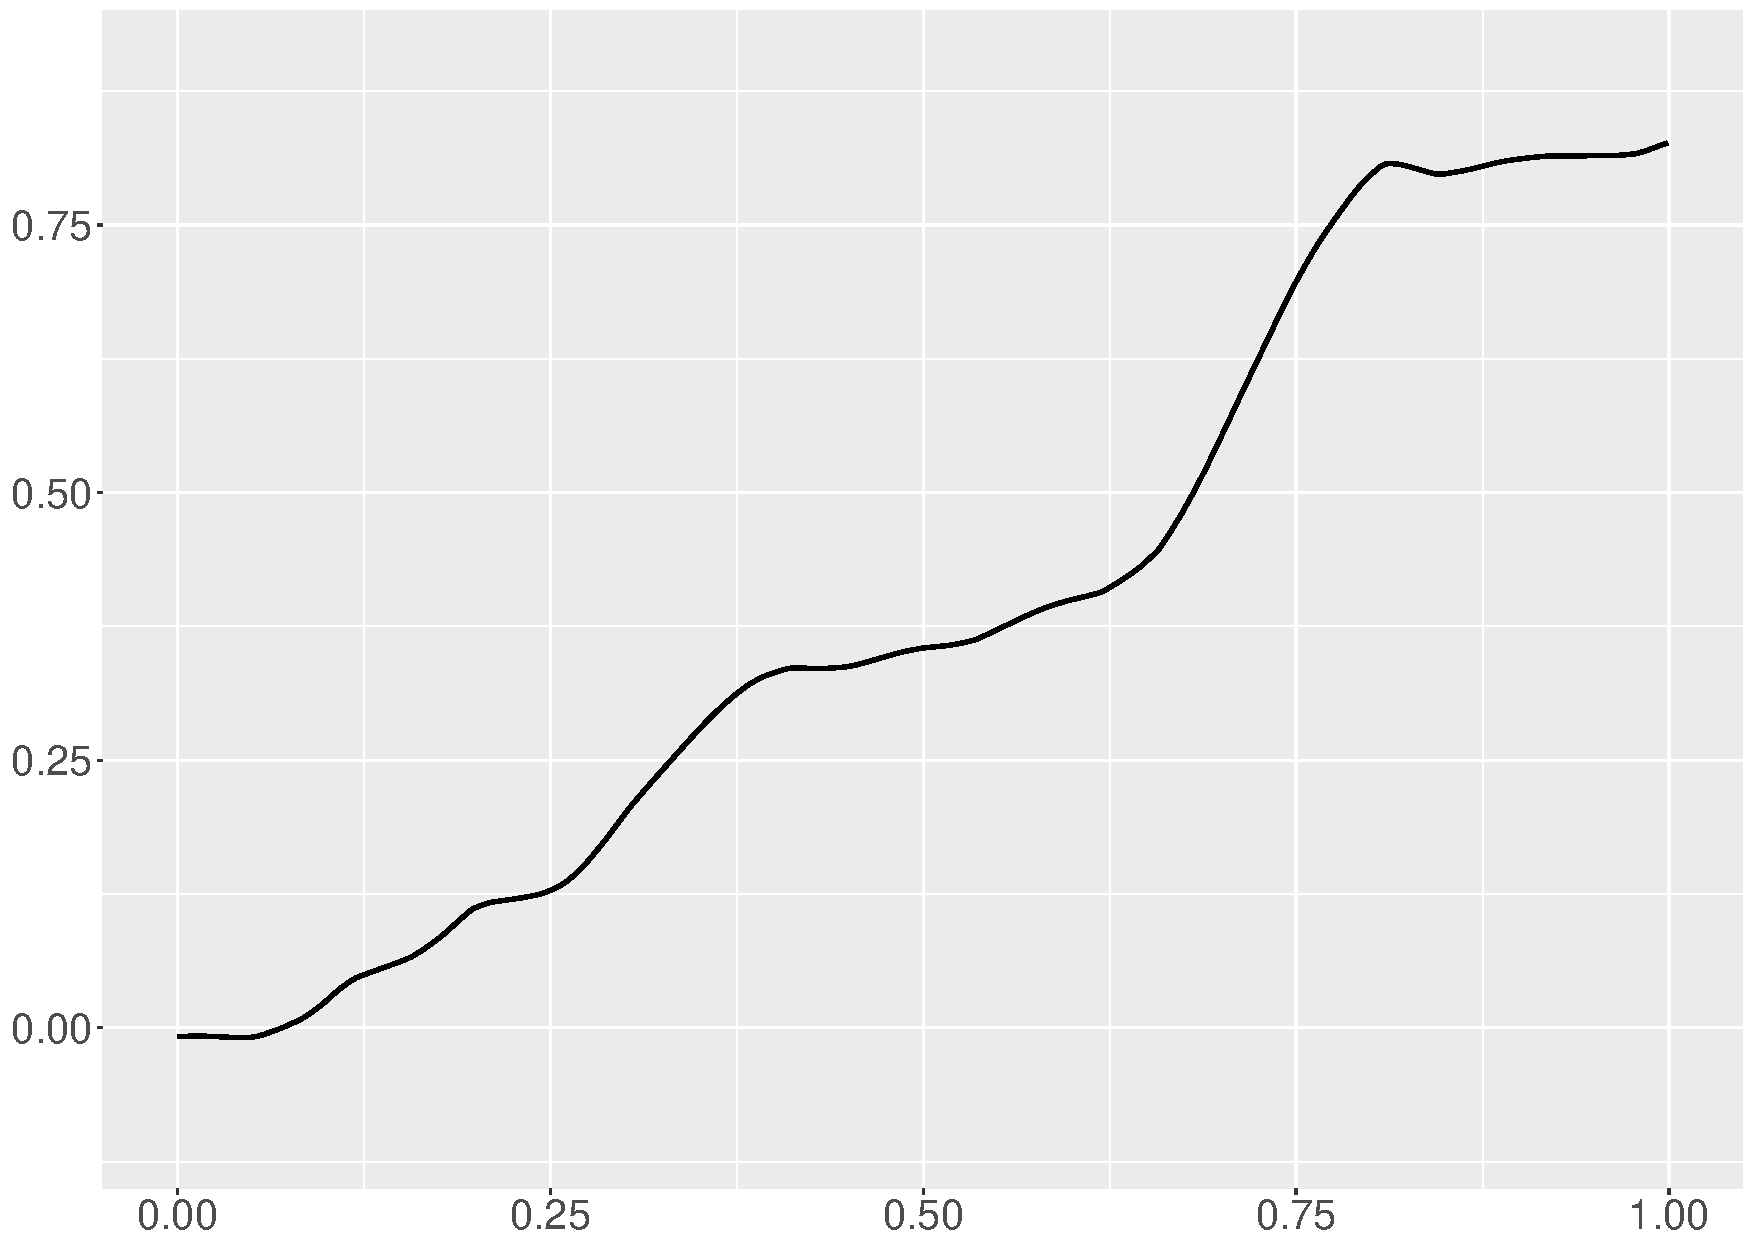
\includegraphics[width=\linewidth,height=0.45\textwidth]{Chapters/02TractorSplineTheory/plot/ggplot/ggBlocksGamma.pdf}
    \caption{Reconstruction by Tractor Spline setting $\gamma=0$}
    \end{subfigure}
  \begin{subfigure}{0.45\textwidth}
    \centering
    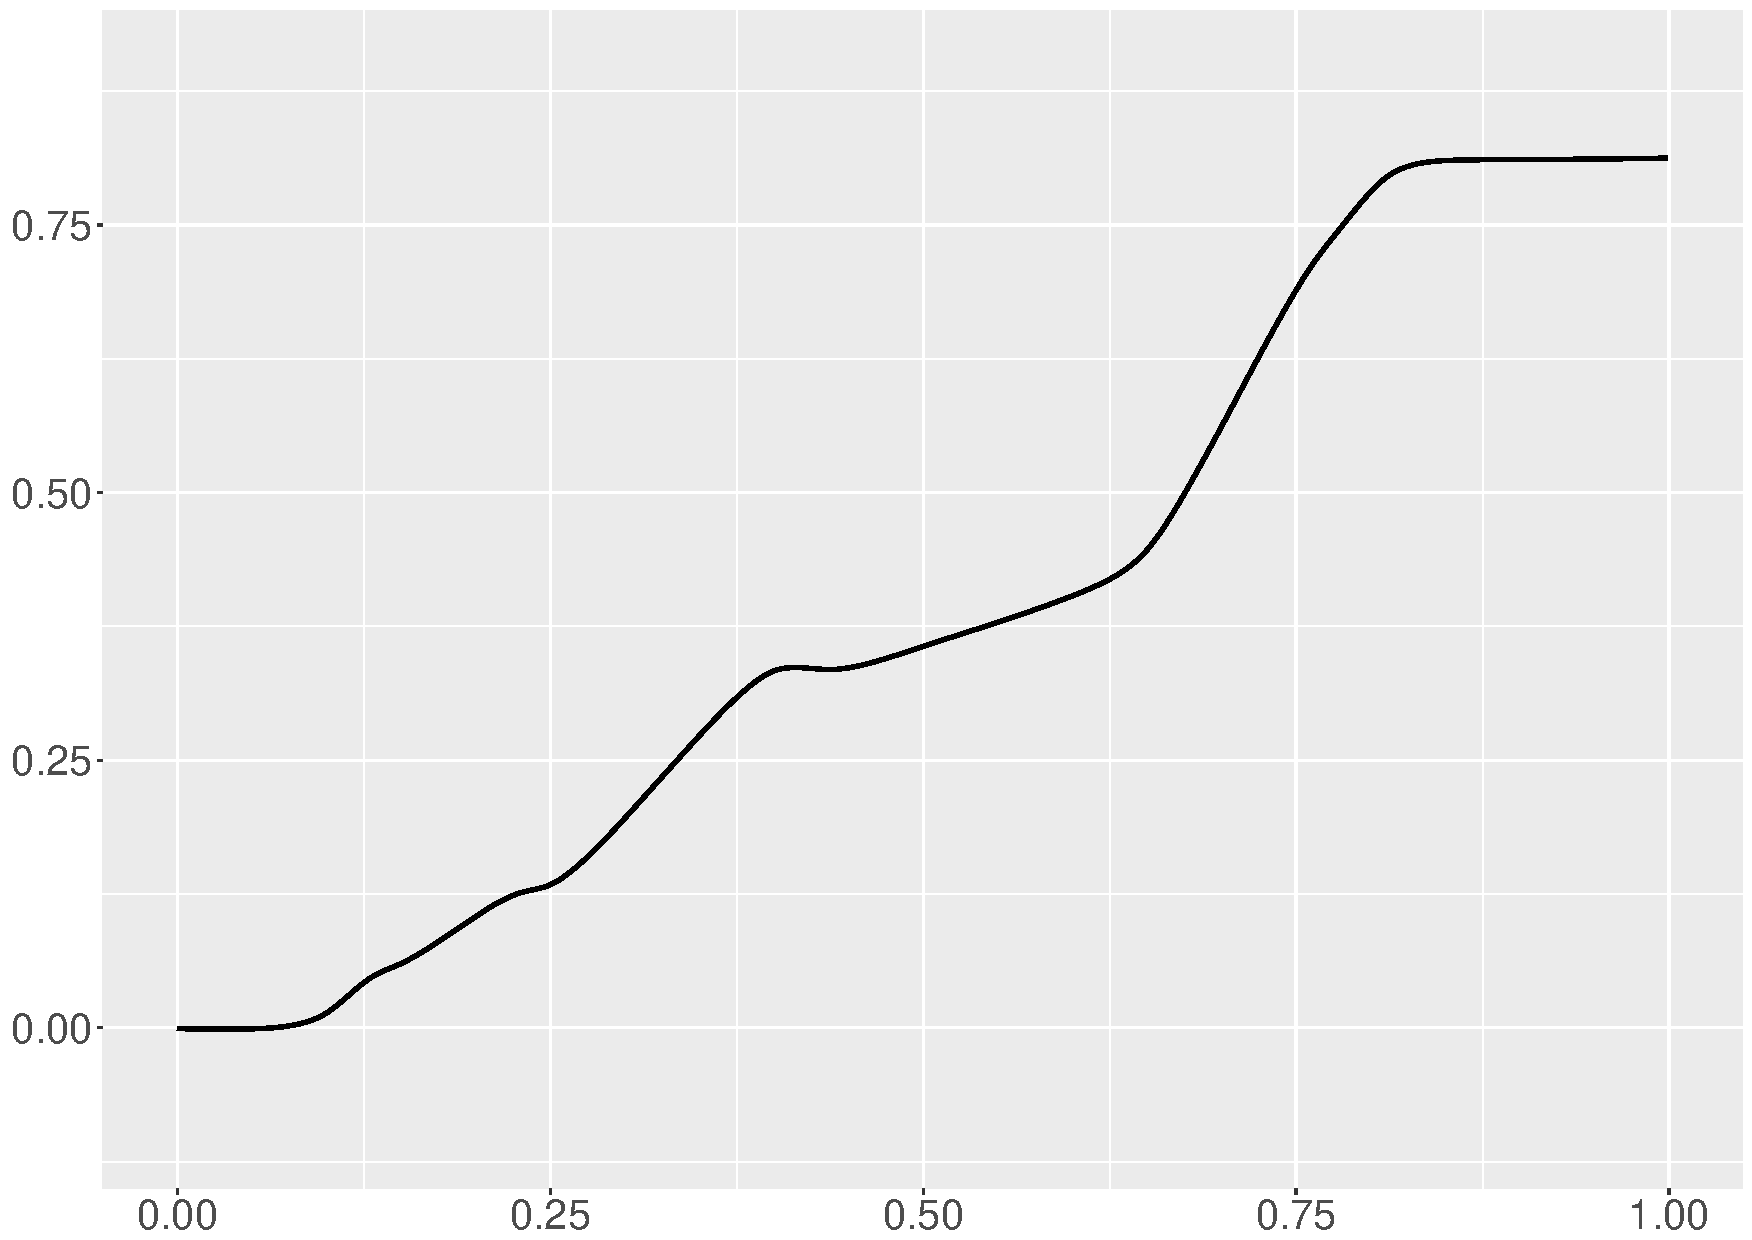
\includegraphics[width=\linewidth,height=0.45\textwidth]{Chapters/02TractorSplineTheory/plot/ggplot/ggBlocksTractorAPT.pdf}
    \caption{Reconstruction by Tractor Spline with conventional penalty term.}
    \end{subfigure}
    \begin{subfigure}{0.45\textwidth}
    \centering
    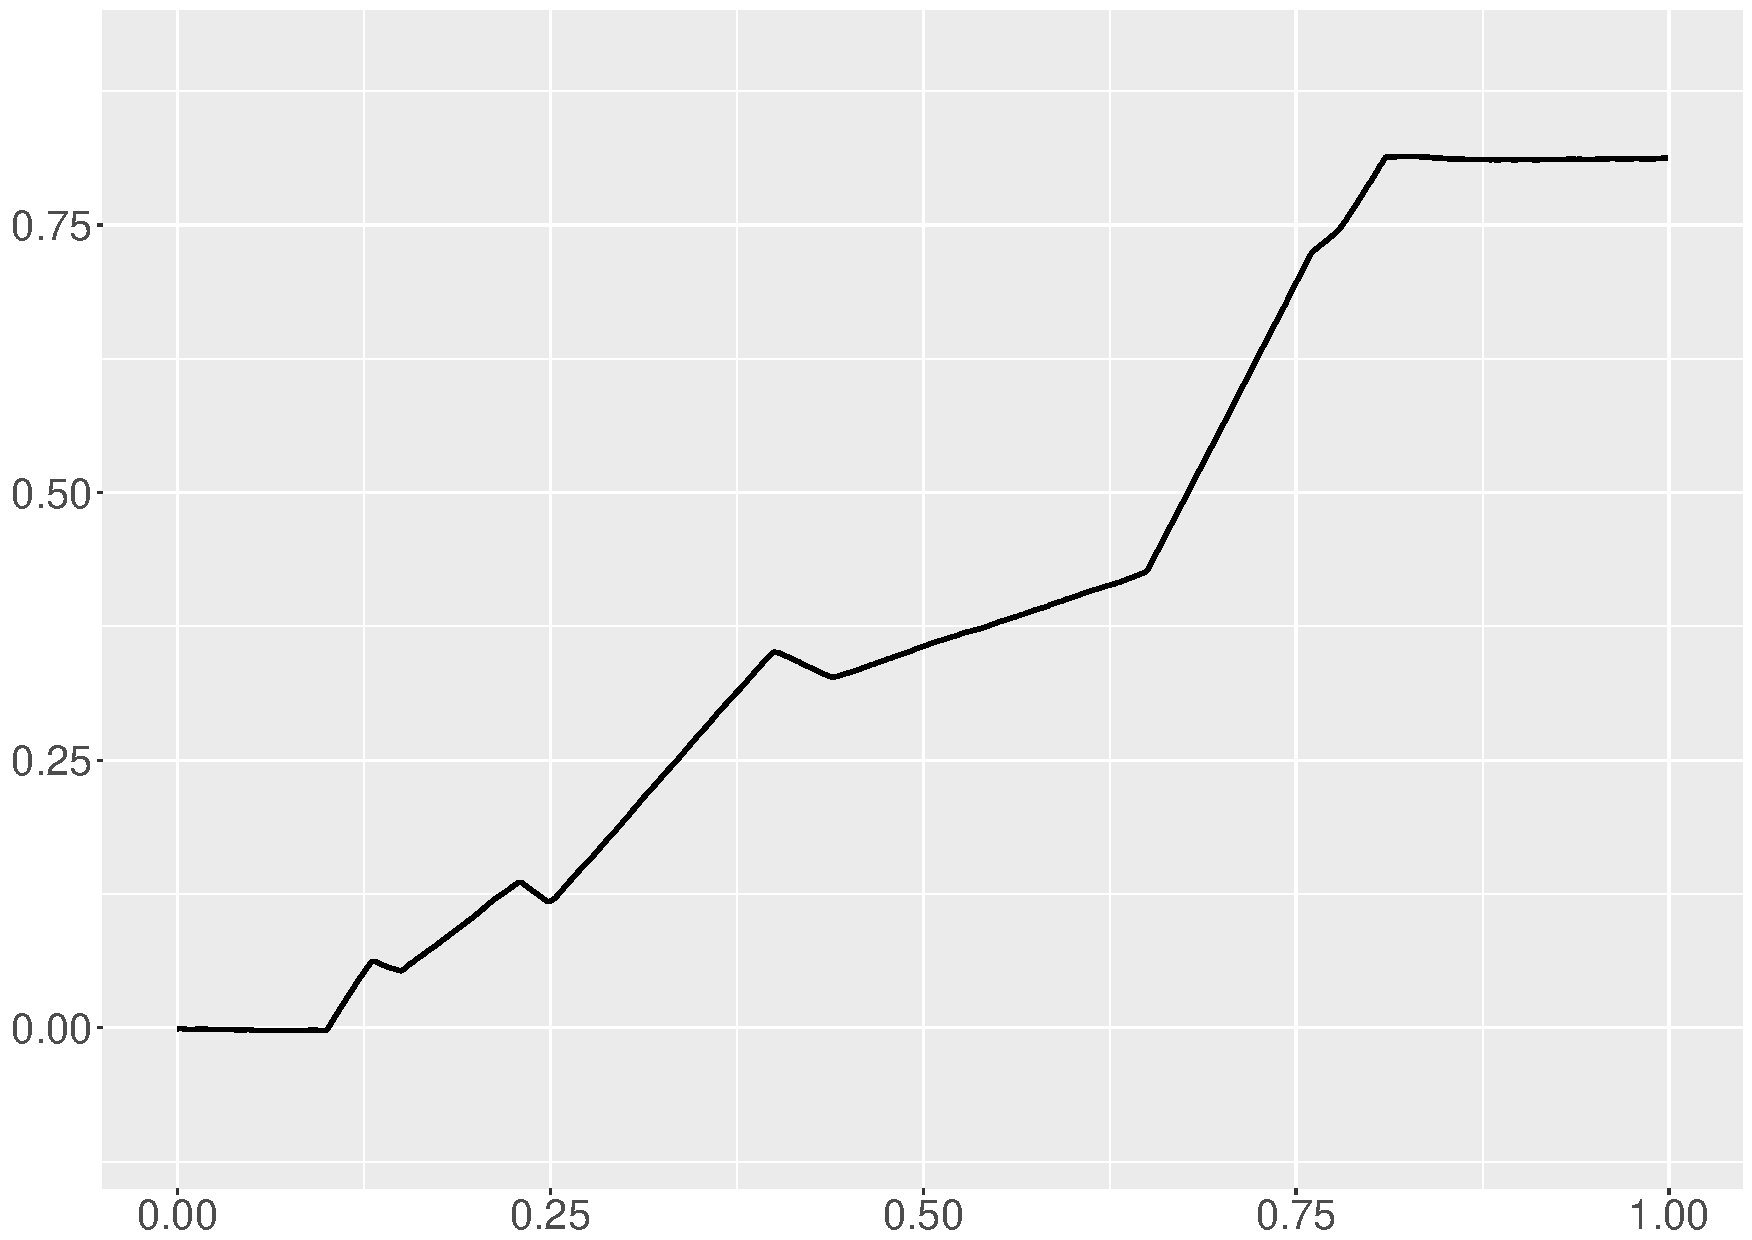
\includegraphics[width=\linewidth,height=0.45\textwidth]{Chapters/02TractorSplineTheory/plot/ggplot/ggBlocksTractor.pdf}
    \caption{Reconstruction by proposed Tractor Spline.}
    \end{subfigure}
\caption{Numerical example: $\textit{Blocks}$. Comparison of different reconstruction methods with simulated data.}\label{num1}
 \end{figure}

%
%\begin{figure}
%  \centering
%    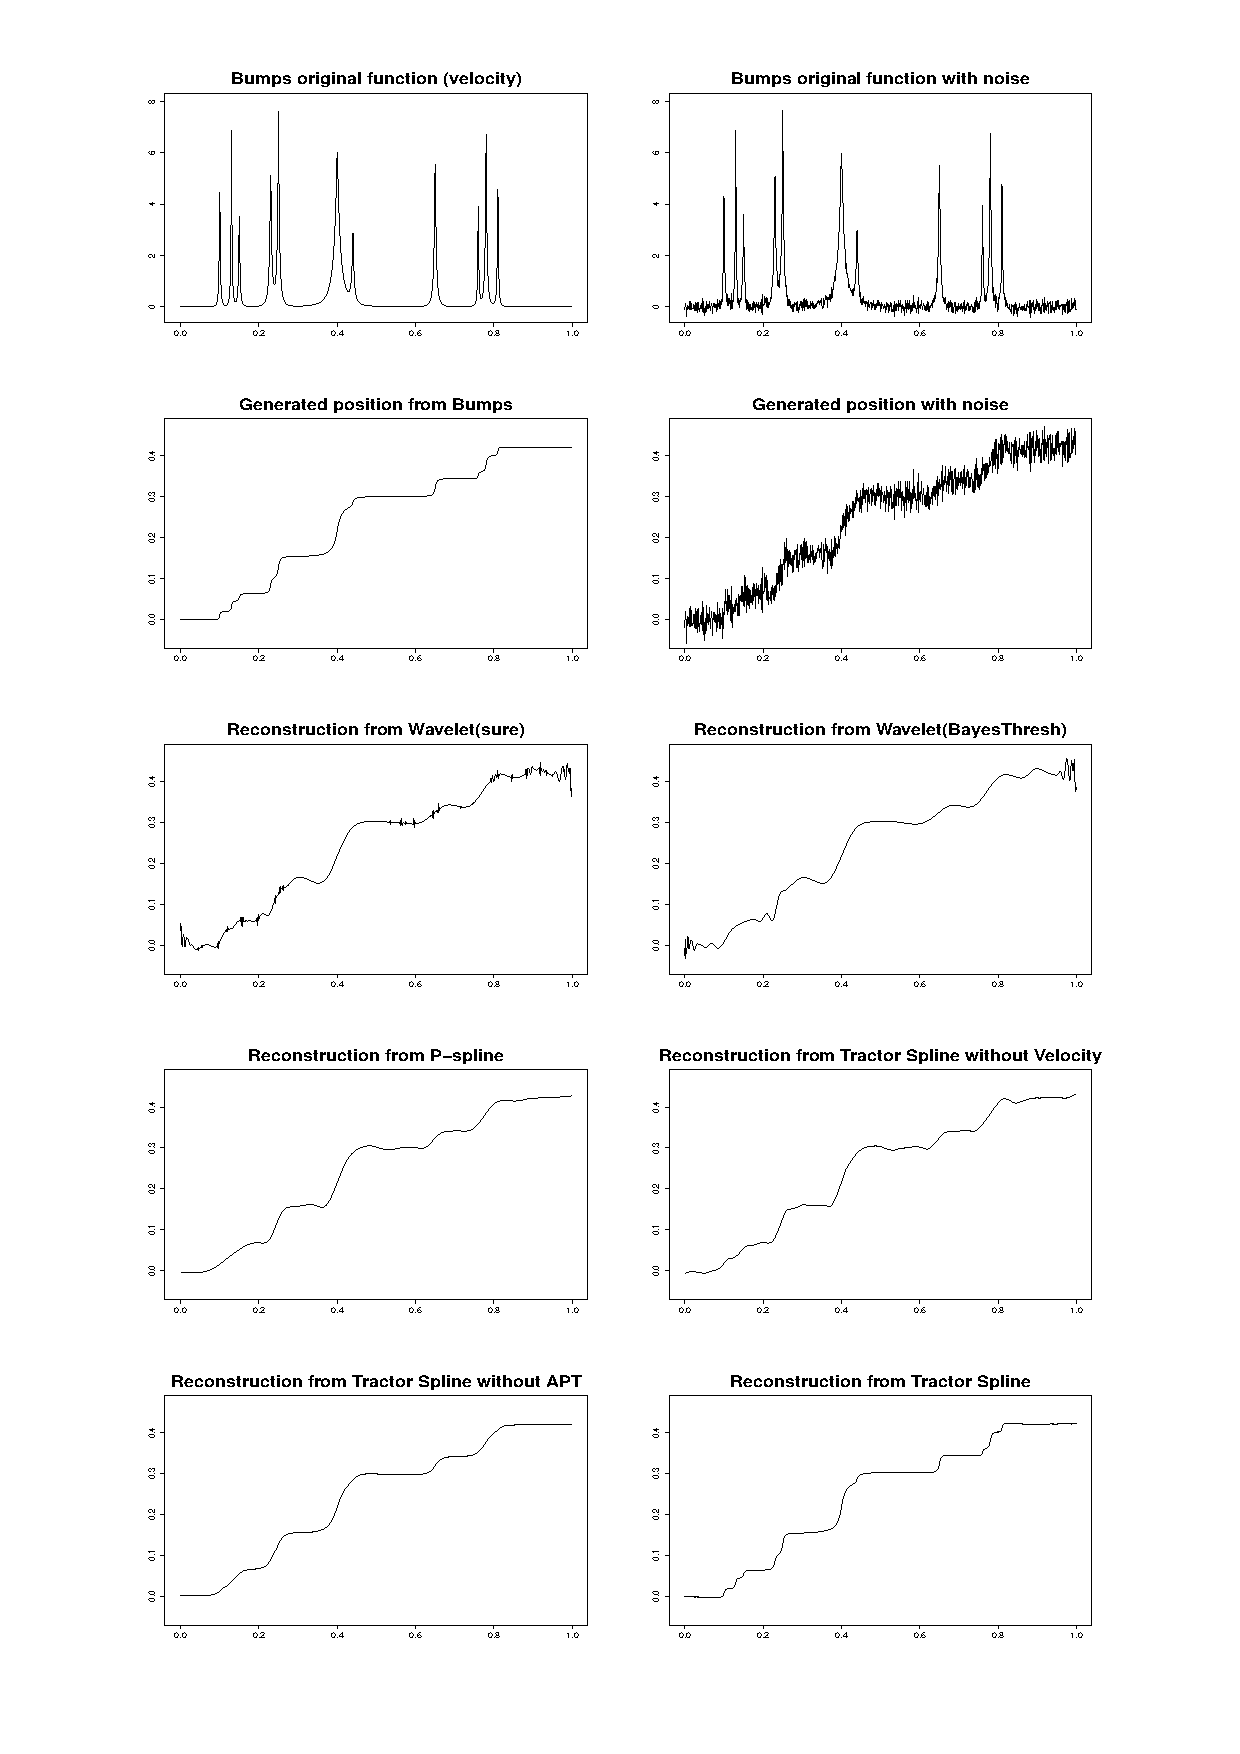
\includegraphics[width=\textwidth,height=14cm]{Chapters/02TractorSplineTheory/plot/bumps10}
%  \caption{Numerical example: $\textit{Bumps}$. (a) The true velocity function. (b) Velocity with Gaussian noise at SNR=7. (c) Generated position function. (d) Position with Gaussian noise at SNR=7. (e) Reconstruction from Wavelet with sure threshold. (f) Reconstruction from Wavelet with BayesThresh approach. (g) Reconstruction by P-spline. (h) Reconstruction by Tractor Spline setting $\gamma=0$. (i) Reconstruction by Tractor Spline with normal penalty term. (j) Reconstruction by proposed Tractor Spline.}\label{num2}
%\end{figure}


\begin{figure}
    \centering
    \begin{subfigure}{0.45\textwidth}
    \centering
    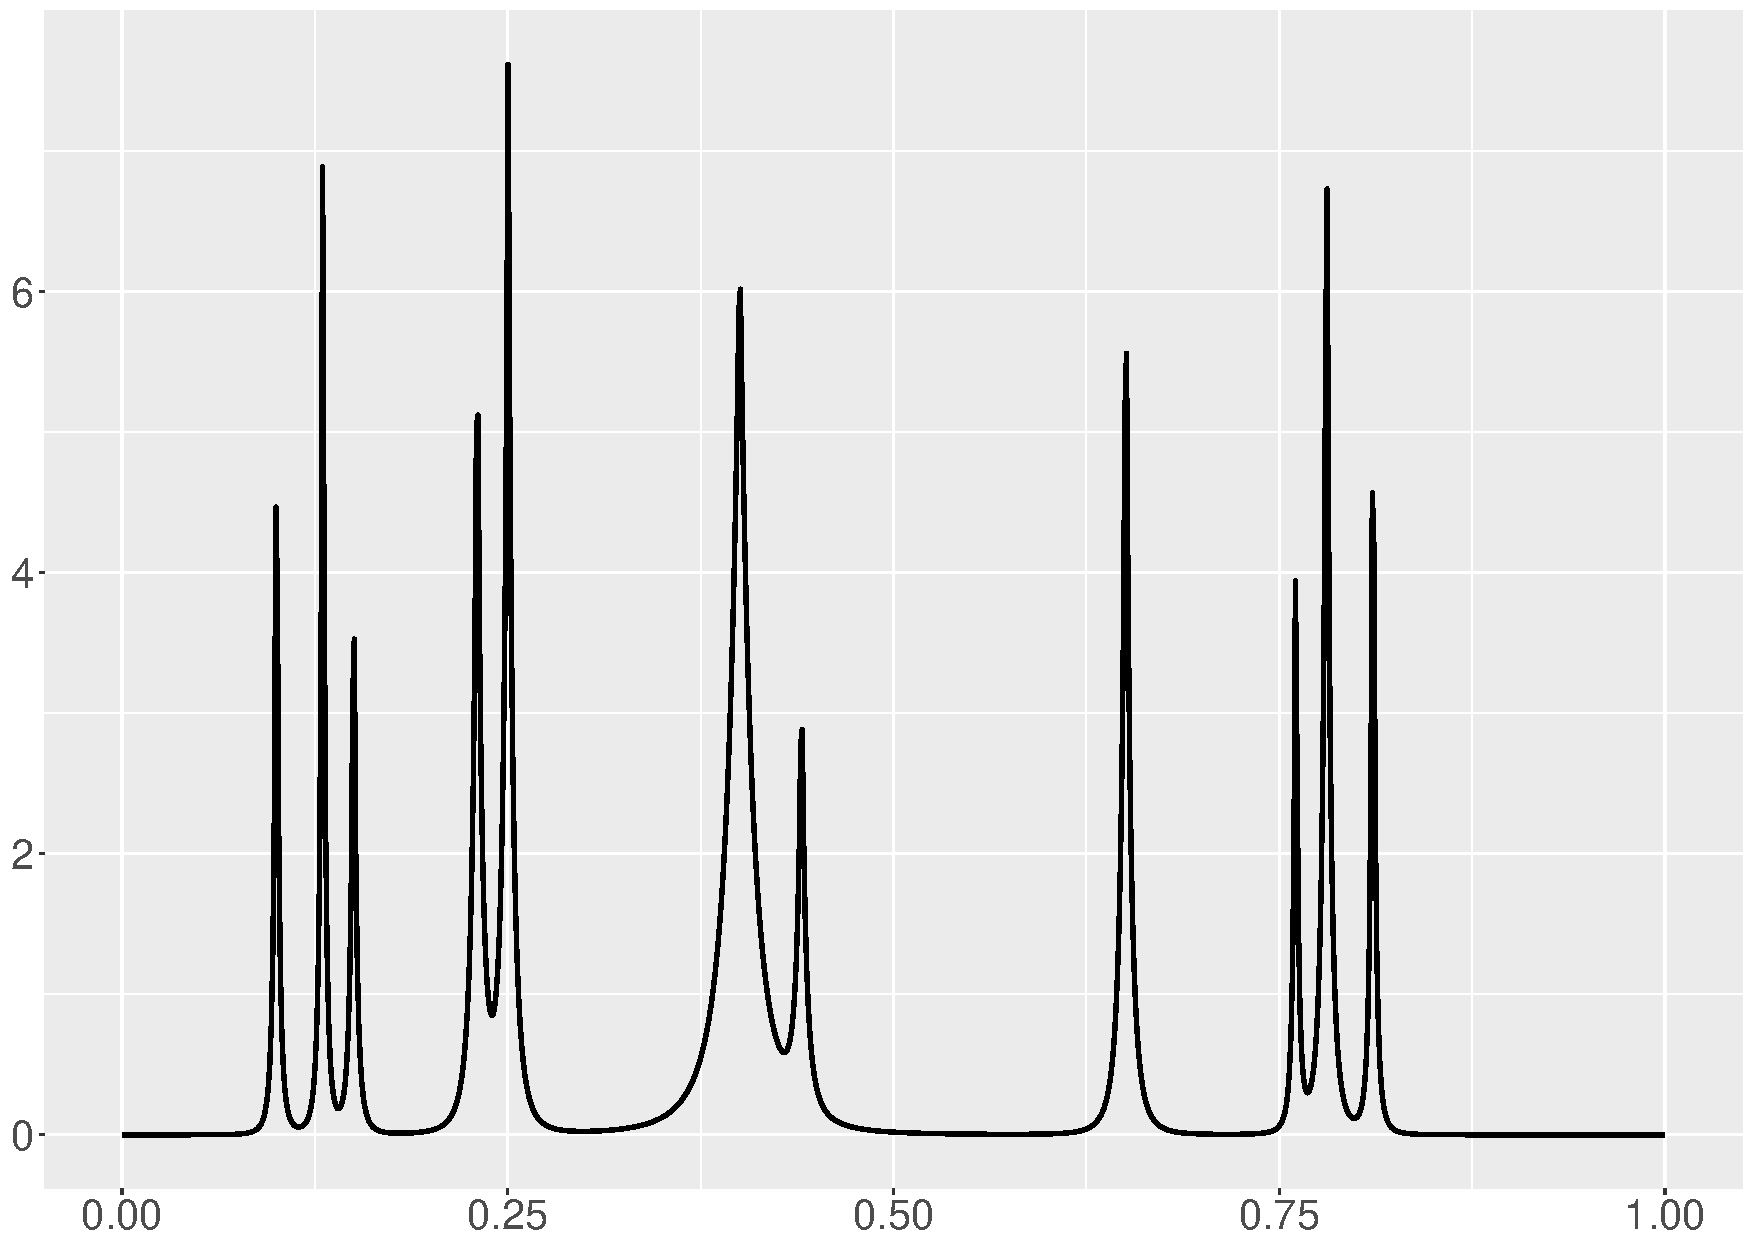
\includegraphics[width=\linewidth,height=0.45\textwidth]{Chapters/02TractorSplineTheory/plot/ggplot/ggBumps.pdf}
    \caption{True \textit{Bumps} function.}
    \end{subfigure}%
    \begin{subfigure}{0.45\textwidth}
    \centering
    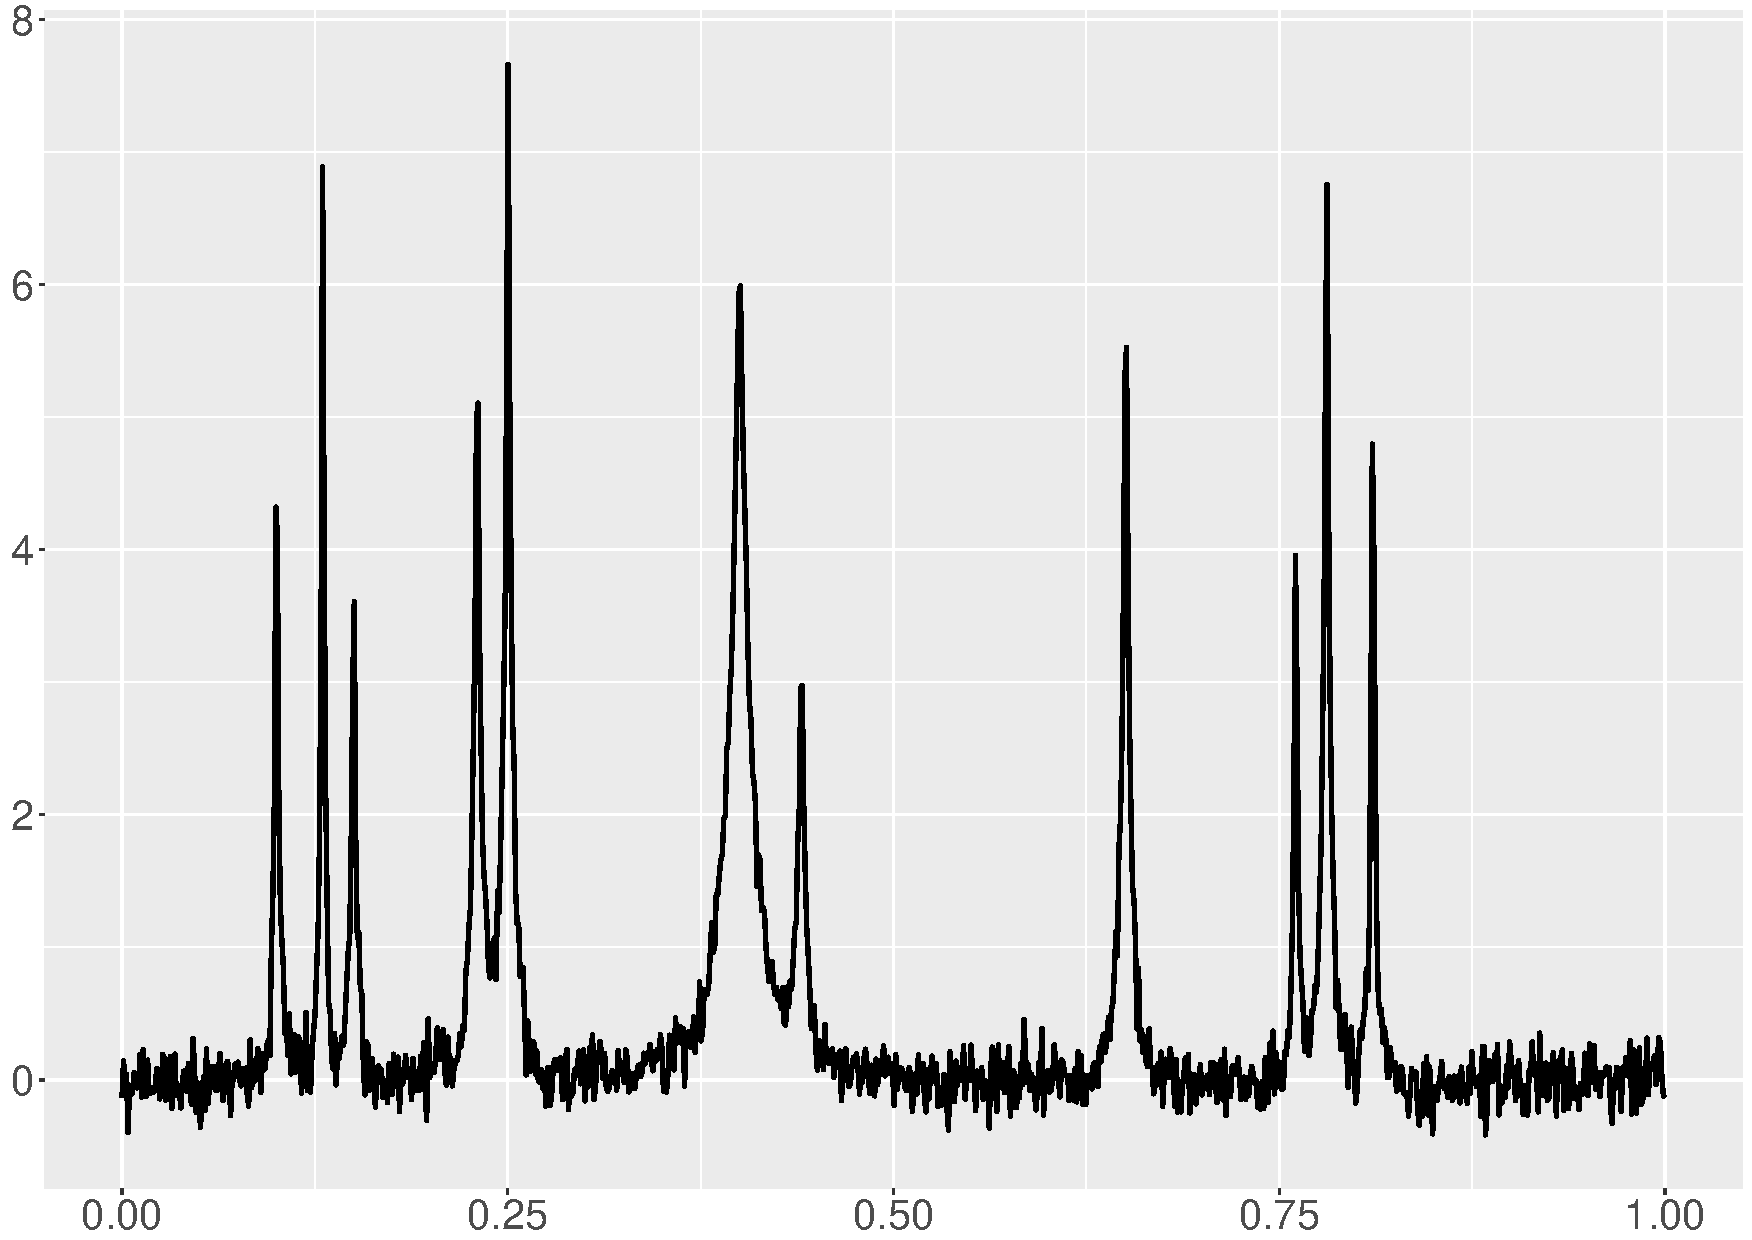
\includegraphics[width=\linewidth,,height=0.45\textwidth]{Chapters/02TractorSplineTheory/plot/ggplot/ggBumpsNoise.pdf}
    \caption{Noisy \textit{Bumps} at \textit{SNR}=7.}
    \end{subfigure}
    \begin{subfigure}{0.45\textwidth}
    \centering
    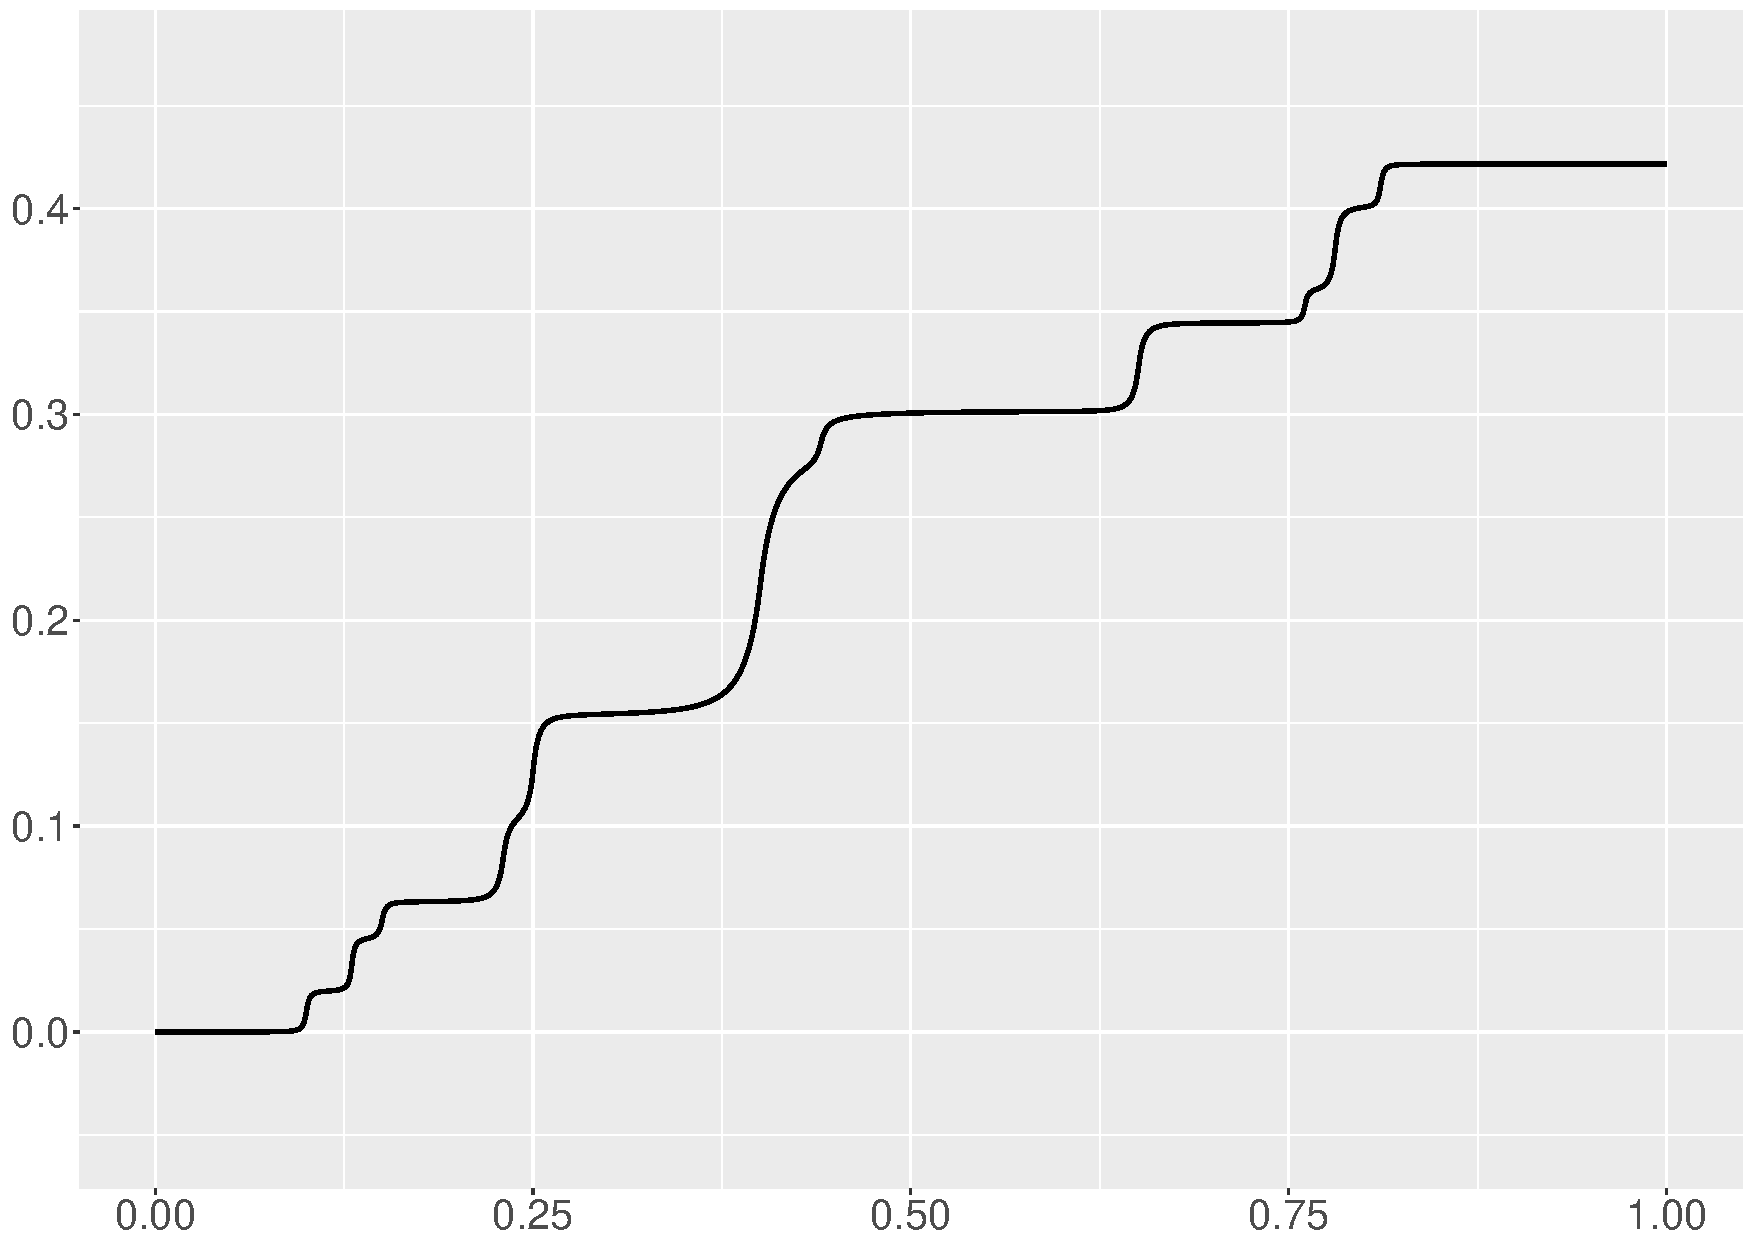
\includegraphics[width=\linewidth,height=0.45\textwidth]{Chapters/02TractorSplineTheory/plot/ggplot/ggBumpsPosition.pdf}
    \caption{Generated positions.}
    \end{subfigure}
    \begin{subfigure}{0.45\textwidth}
    \centering
    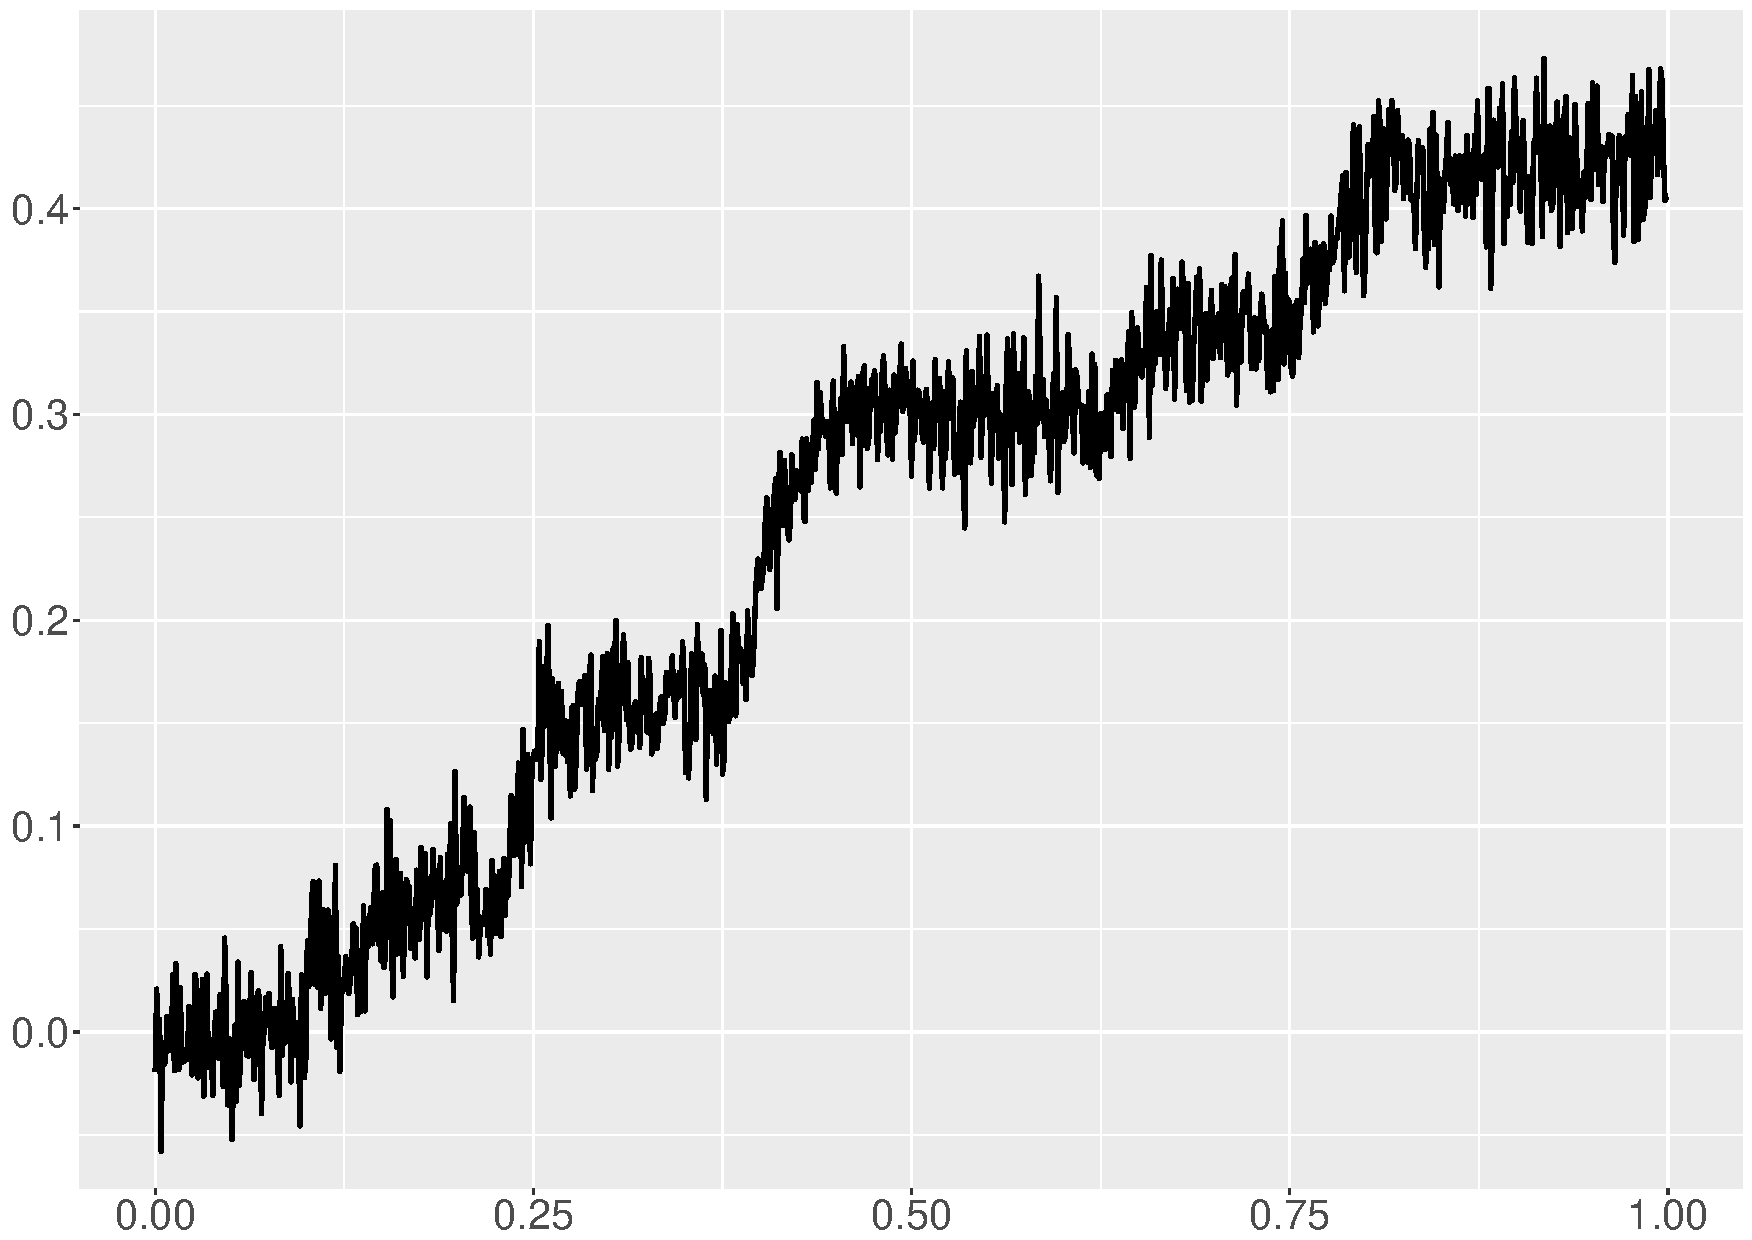
\includegraphics[width=\linewidth,height=0.45\textwidth]{Chapters/02TractorSplineTheory/plot/ggplot/ggBumpsPositionNoise.pdf}
    \caption{Noisy position at \textit{SNR}=7.}
    \end{subfigure}
    \begin{subfigure}{0.45\textwidth}
    \centering
    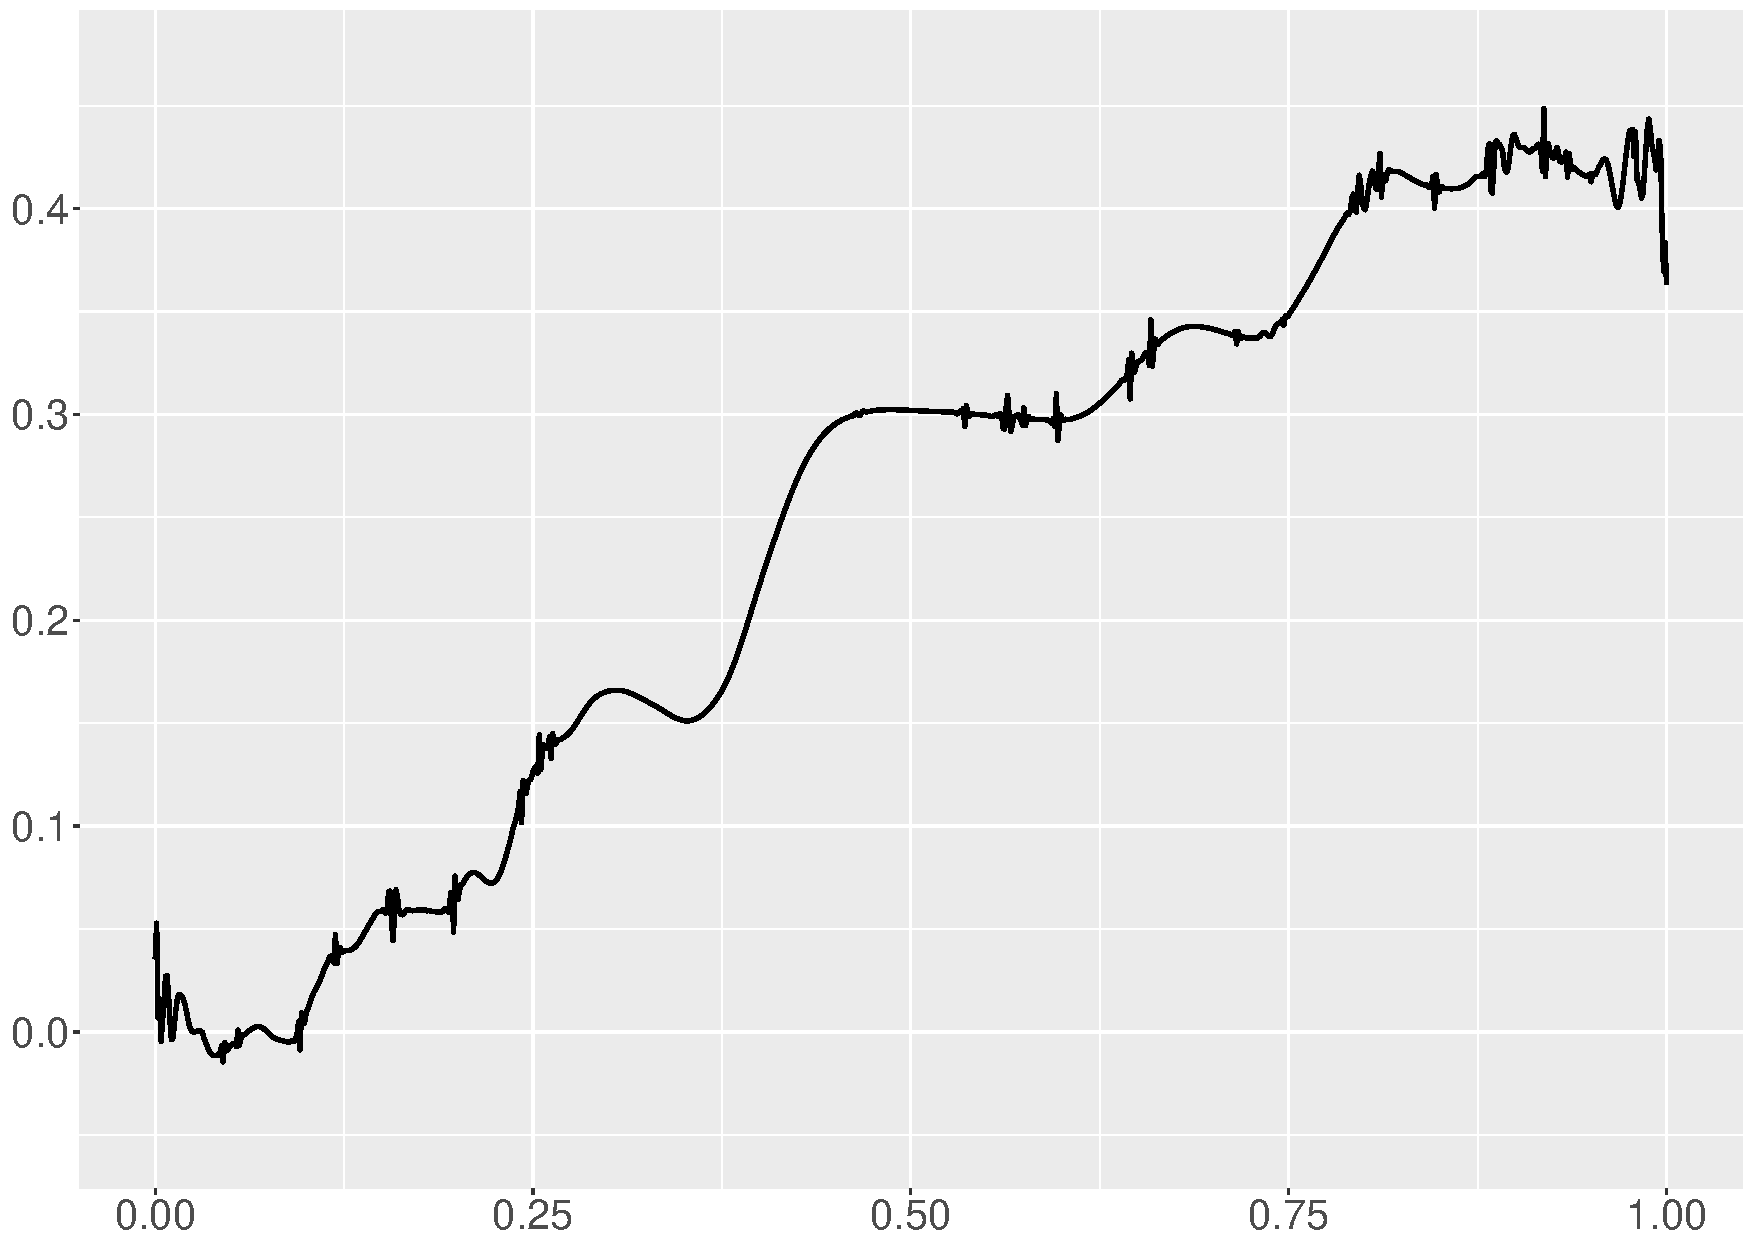
\includegraphics[width=\linewidth,height=0.45\textwidth]{Chapters/02TractorSplineTheory/plot/ggplot/ggBumpsSure.pdf}
    \caption{Reconstruction from Wavelet by sure threshold.}
    \end{subfigure}
    \begin{subfigure}{0.45\textwidth}
    \centering
    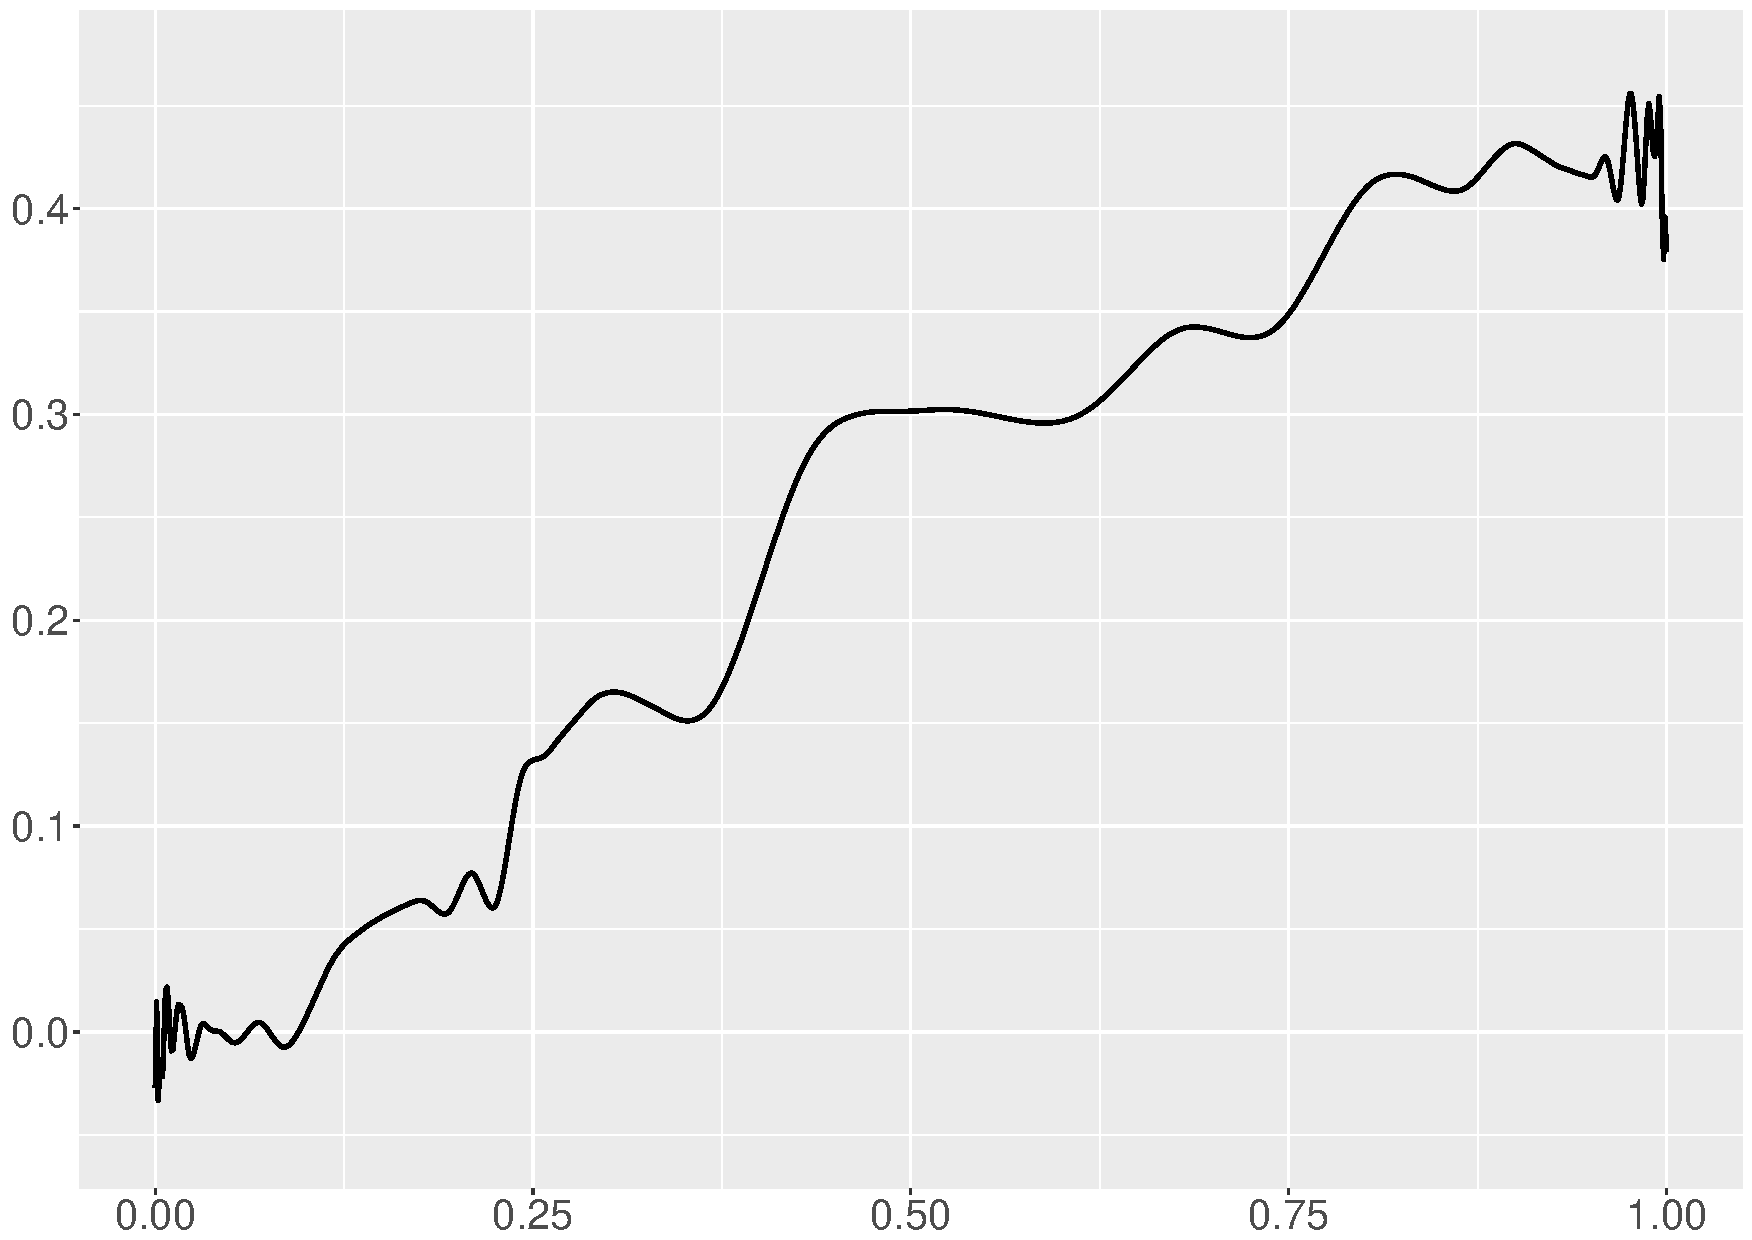
\includegraphics[width=\linewidth,height=0.45\textwidth]{Chapters/02TractorSplineTheory/plot/ggplot/ggBumpsBayes.pdf}
    \caption{Reconstruction from Wavelet by BayesThresh approach.}
    \end{subfigure}
    \begin{subfigure}{0.45\textwidth}
    \centering
    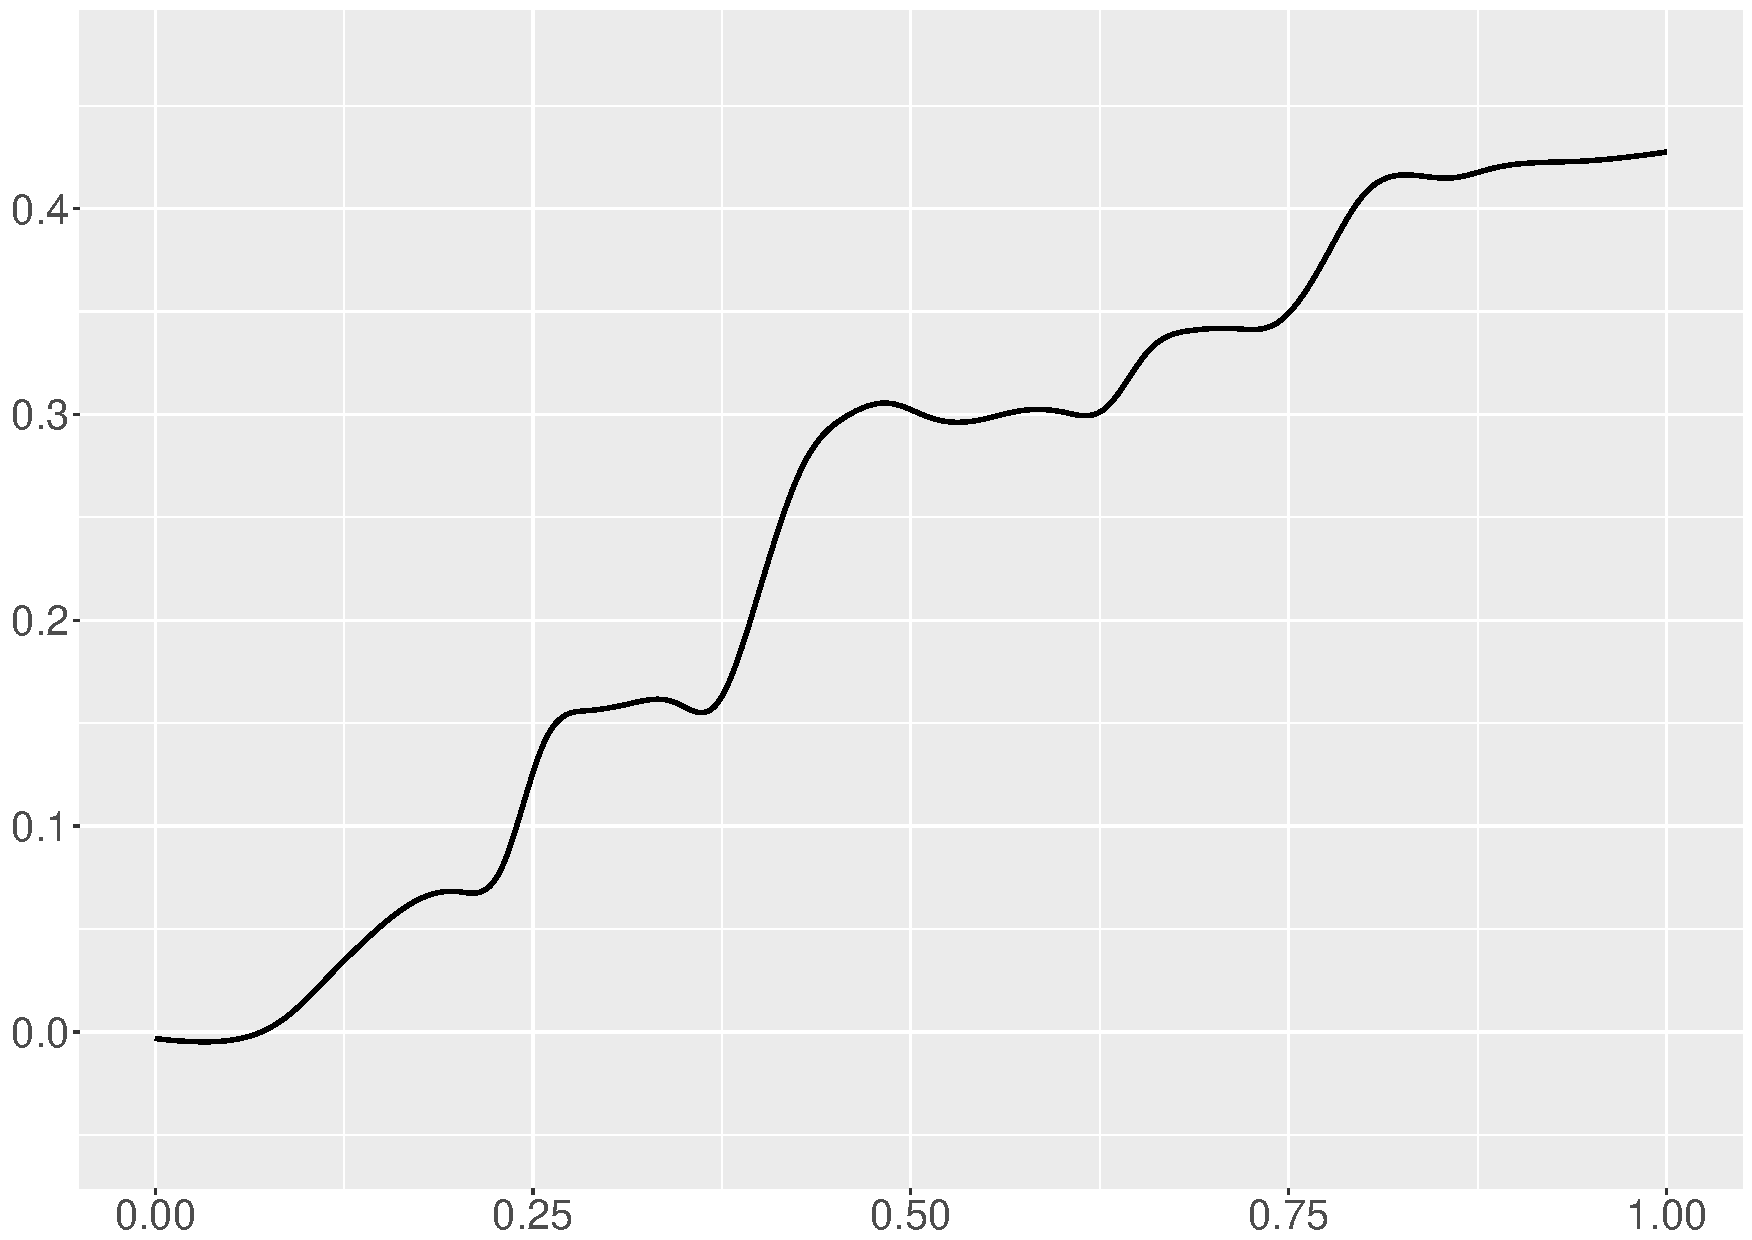
\includegraphics[width=\linewidth,height=0.45\textwidth]{Chapters/02TractorSplineTheory/plot/ggplot/ggBumpsPSpline.pdf}
    \caption{Reconstruction by P-spline. \\\mbox{  } }
    \end{subfigure}
    \begin{subfigure}{0.45\textwidth}
    \centering
    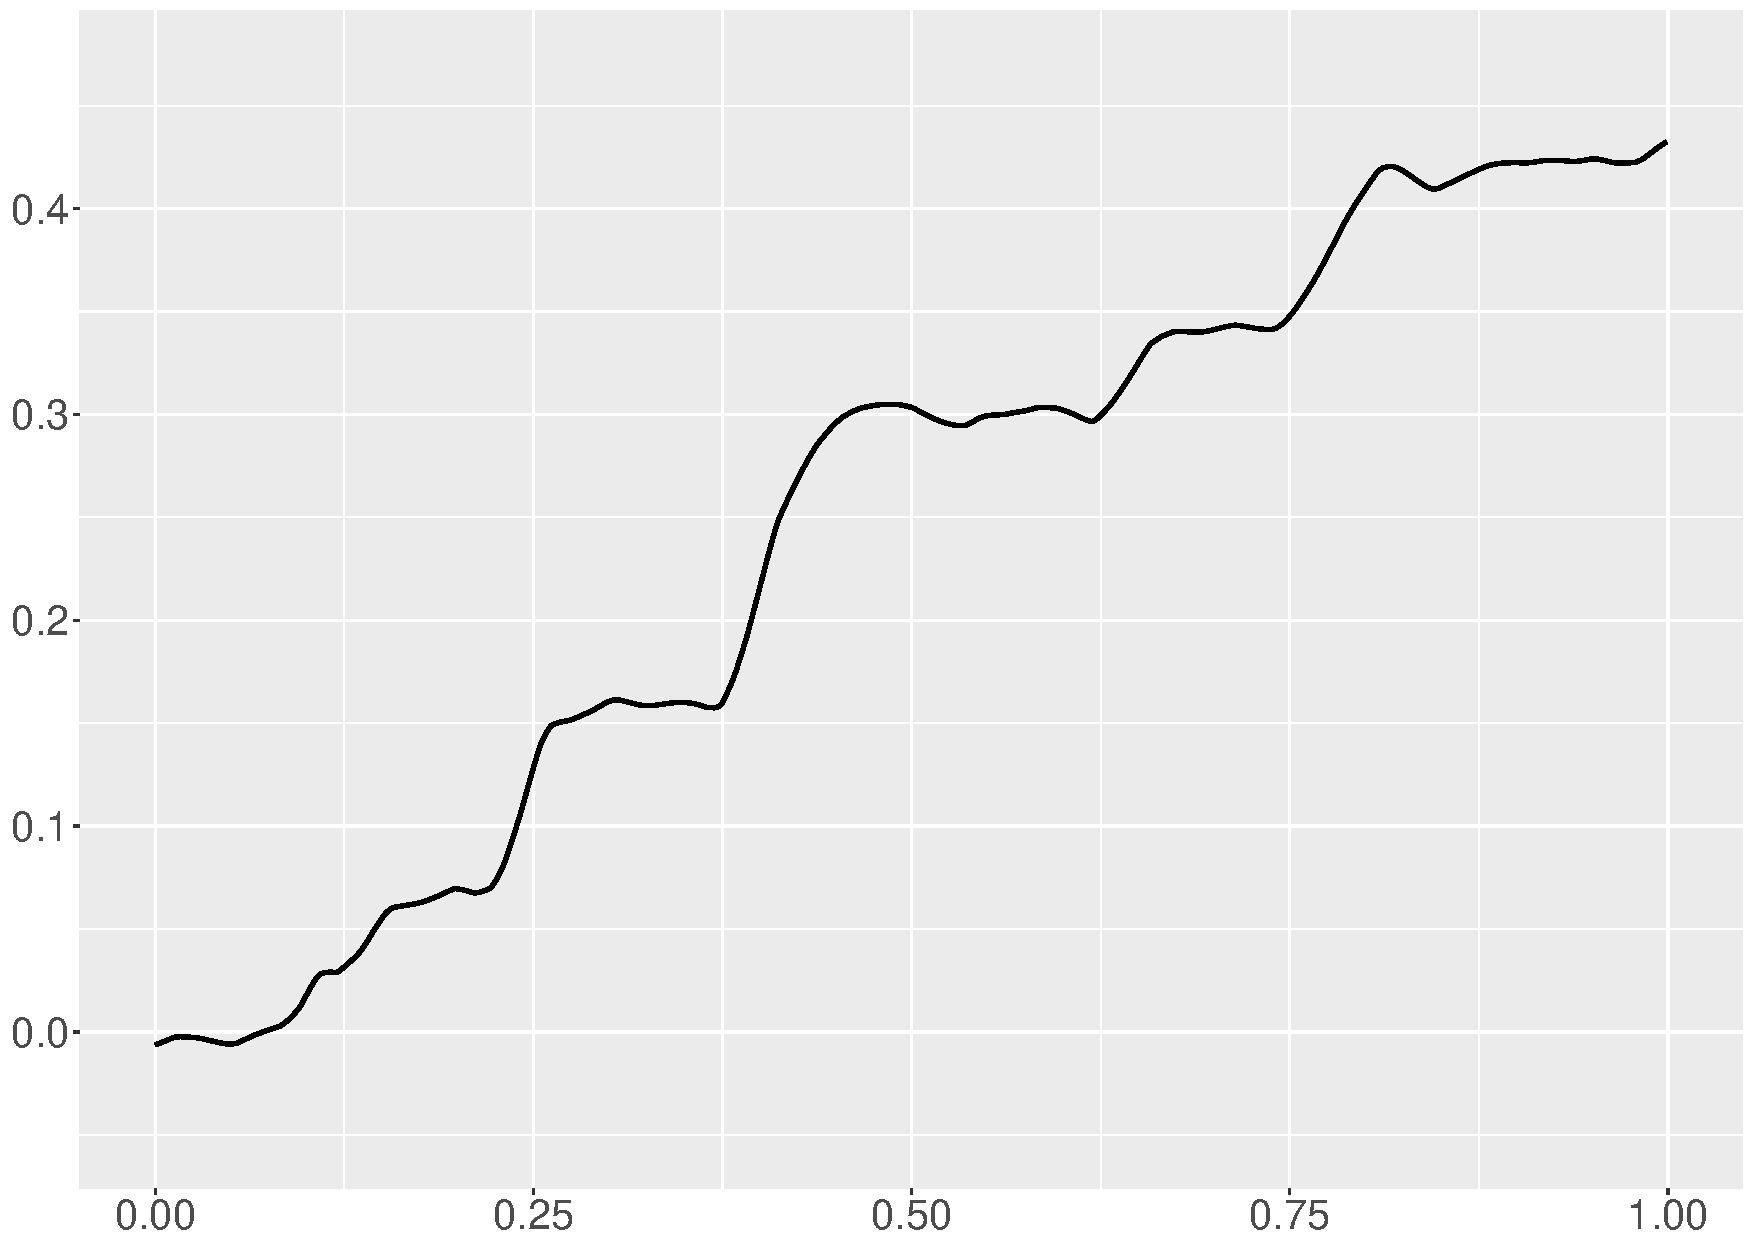
\includegraphics[width=\linewidth,height=0.45\textwidth]{Chapters/02TractorSplineTheory/plot/ggplot/ggBumpsGamma.pdf}
    \caption{Reconstruction by Tractor Spline setting $\gamma=0$}
    \end{subfigure}
  \begin{subfigure}{0.45\textwidth}
    \centering
    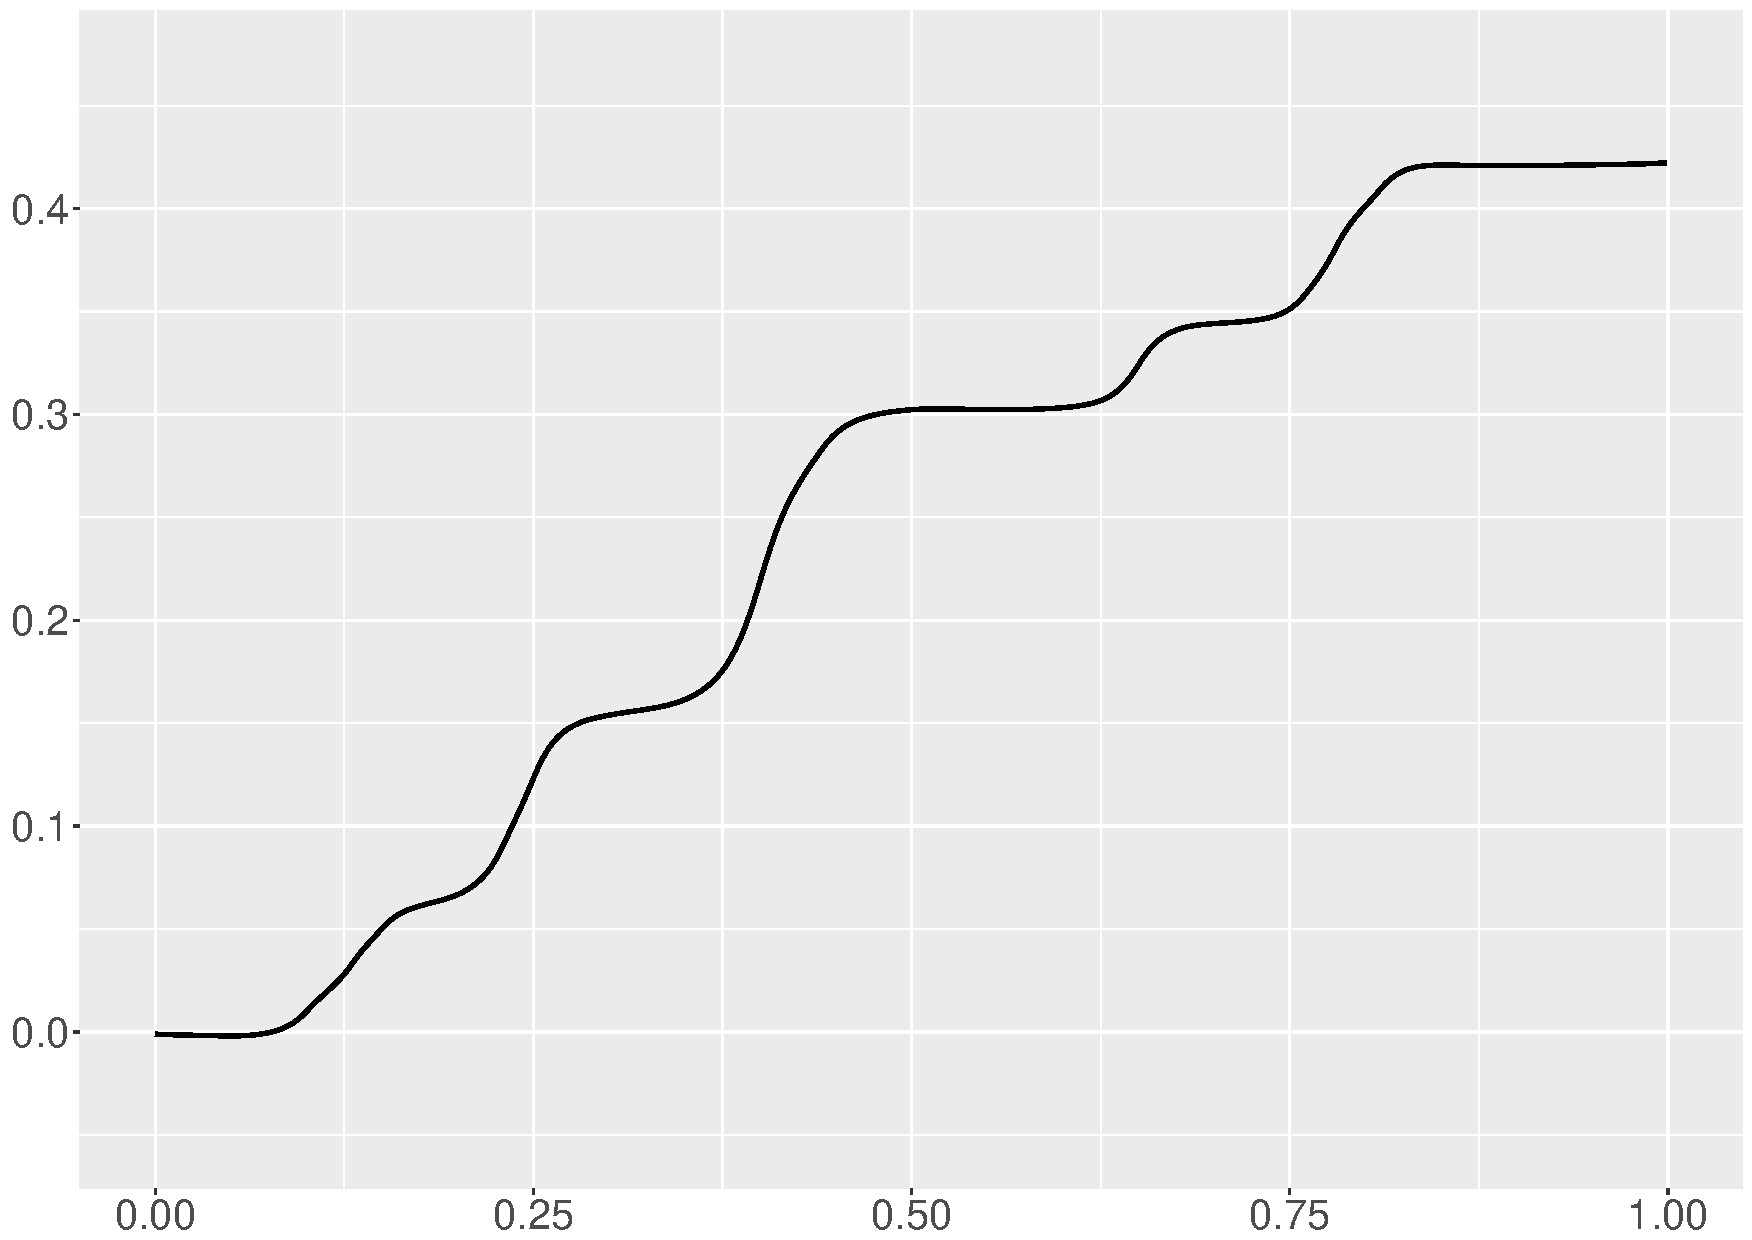
\includegraphics[width=\linewidth,height=0.45\textwidth]{Chapters/02TractorSplineTheory/plot/ggplot/ggBumpsTractorAPT.pdf}
    \caption{Reconstruction by Tractor Spline with conventional penalty term.}
    \end{subfigure}
    \begin{subfigure}{0.45\textwidth}
    \centering
    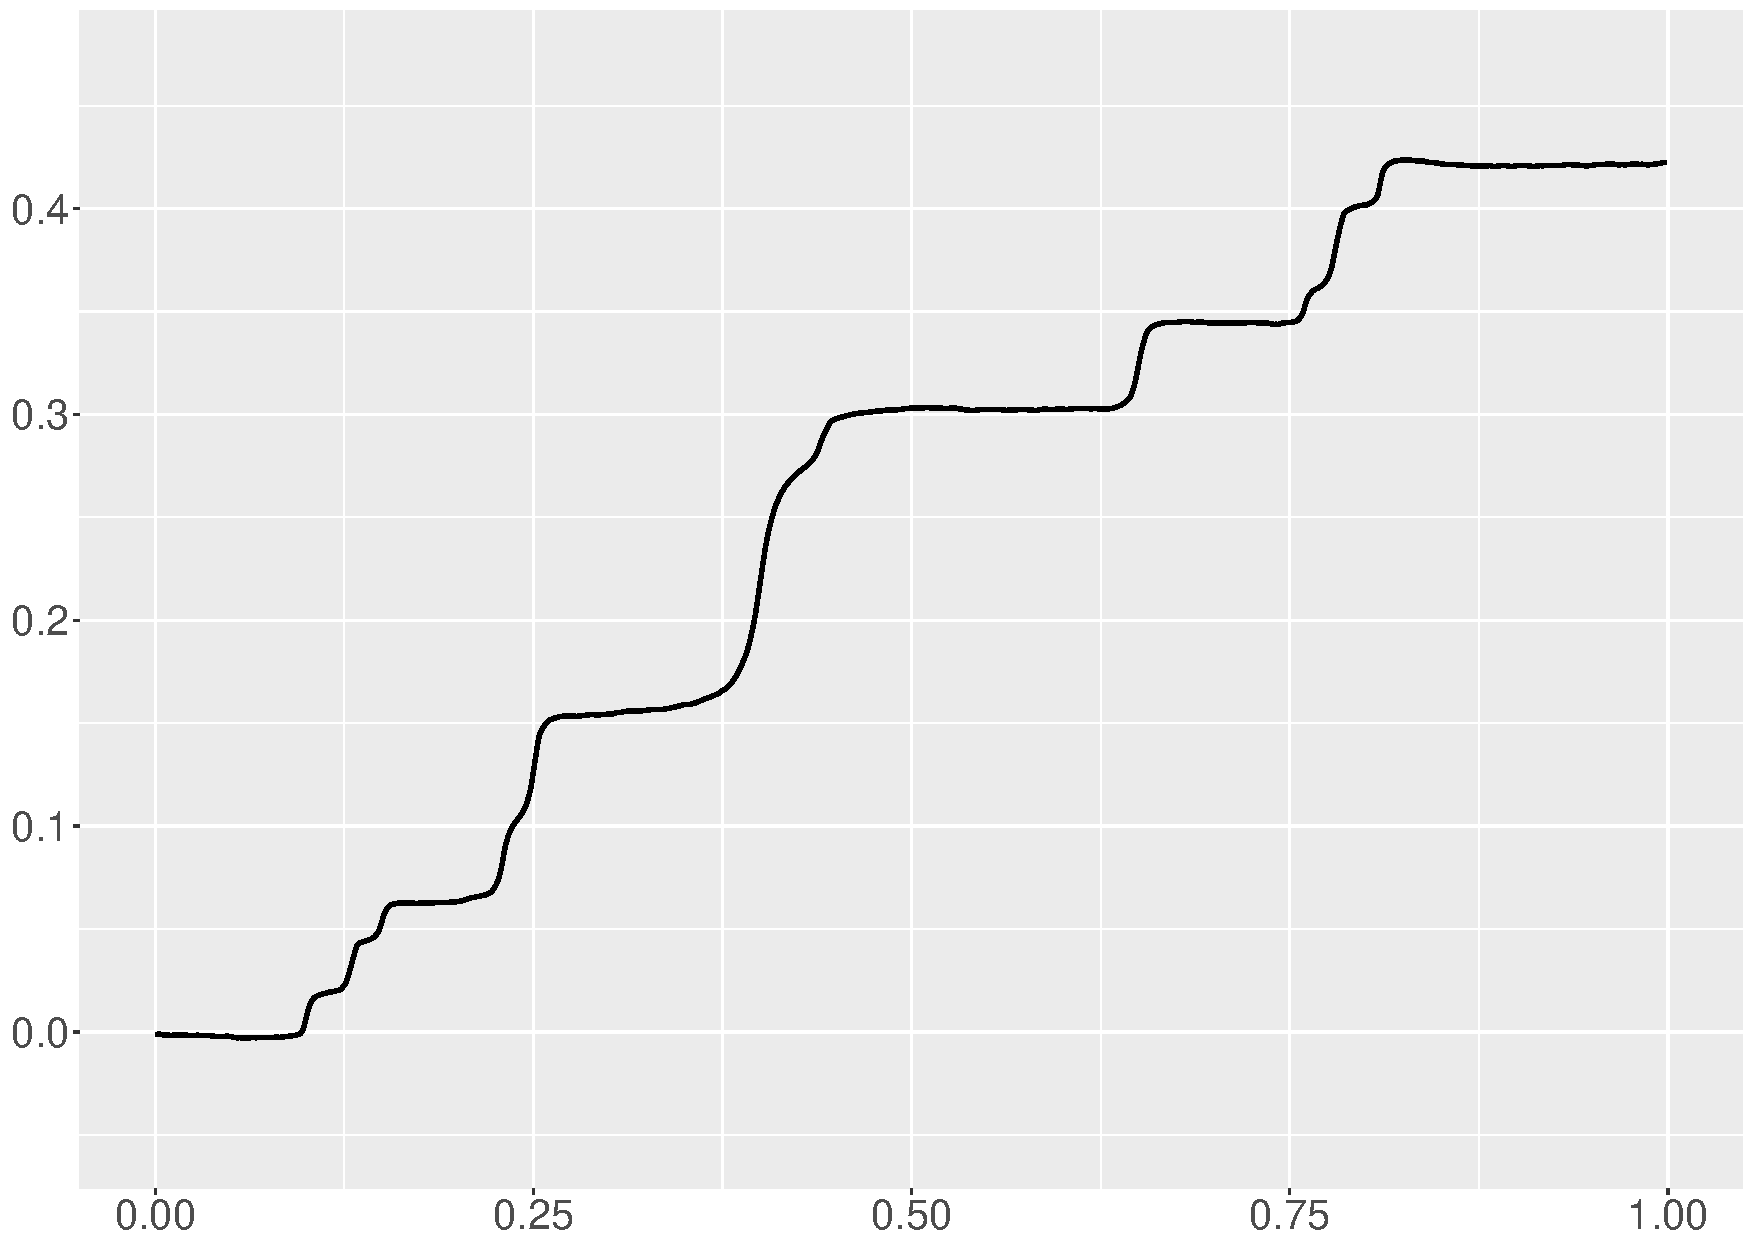
\includegraphics[width=\linewidth,height=0.45\textwidth]{Chapters/02TractorSplineTheory/plot/ggplot/ggBumpsTractor.pdf}
    \caption{Reconstruction by proposed Tractor Spline.}
    \end{subfigure}
\caption{Numerical example: $\textit{Bumps}$. Comparison of different reconstruction methods with simulated data.}\label{num2}
 \end{figure}



%\begin{figure}
%  \centering
%    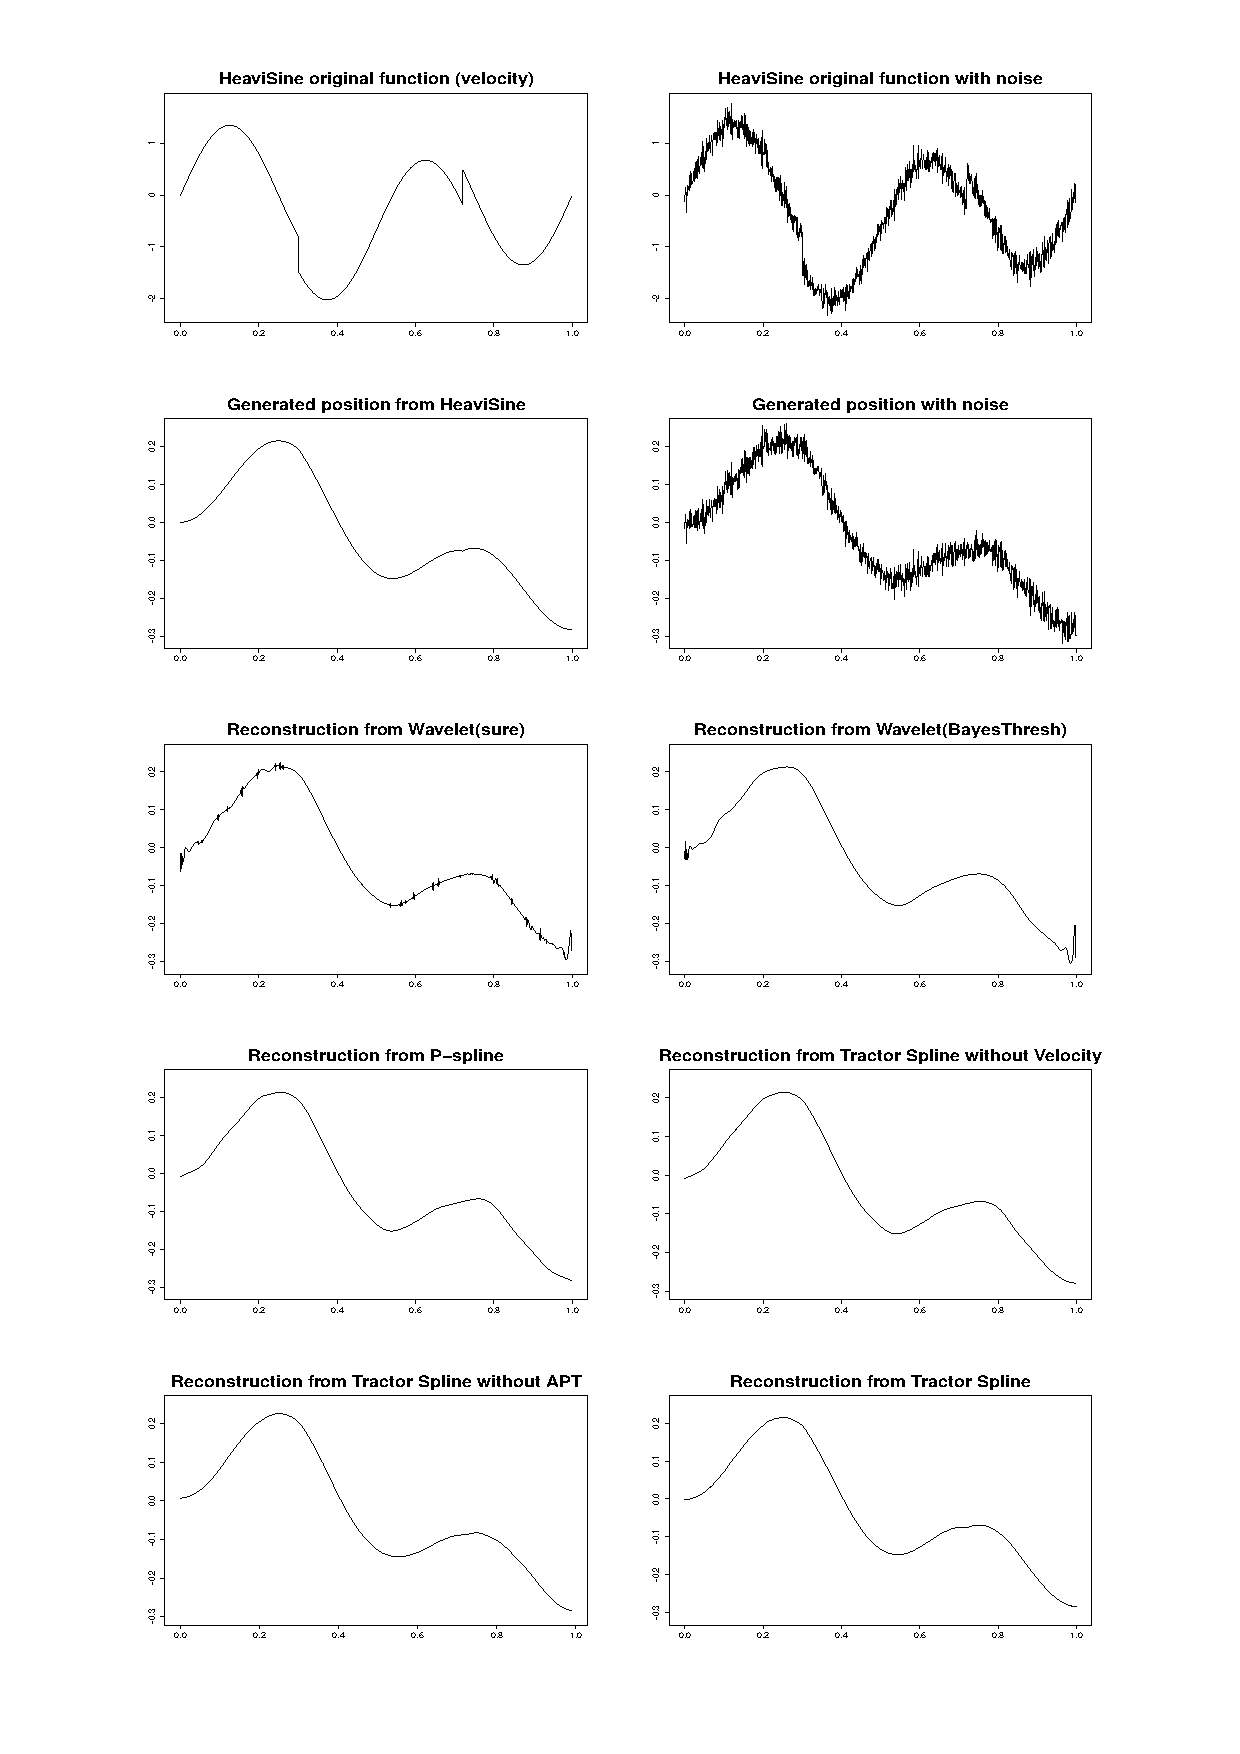
\includegraphics[width=\textwidth,height=14cm]{Chapters/02TractorSplineTheory/plot/heavi10} 
%  \caption{Numerical example: $\textit{HeaviSine}$. (a) The true velocity function. (b) Velocity with Gaussian noise at SNR=7. (c) Generated position function. (d) Position with Gaussian noise at SNR=7. (e) Reconstruction from Wavelet with sure threshold. (f) Reconstruction from Wavelet with BayesThresh approach. (g) Reconstruction by P-spline. (h) Reconstruction by Tractor Spline setting $\gamma=0$. (i) Reconstruction by Tractor Spline with normal penalty term. (j) Reconstruction by proposed Tractor Spline.}\label{num3}
%\end{figure}



\begin{figure}
    \centering
    \begin{subfigure}{0.45\textwidth}
    \centering
    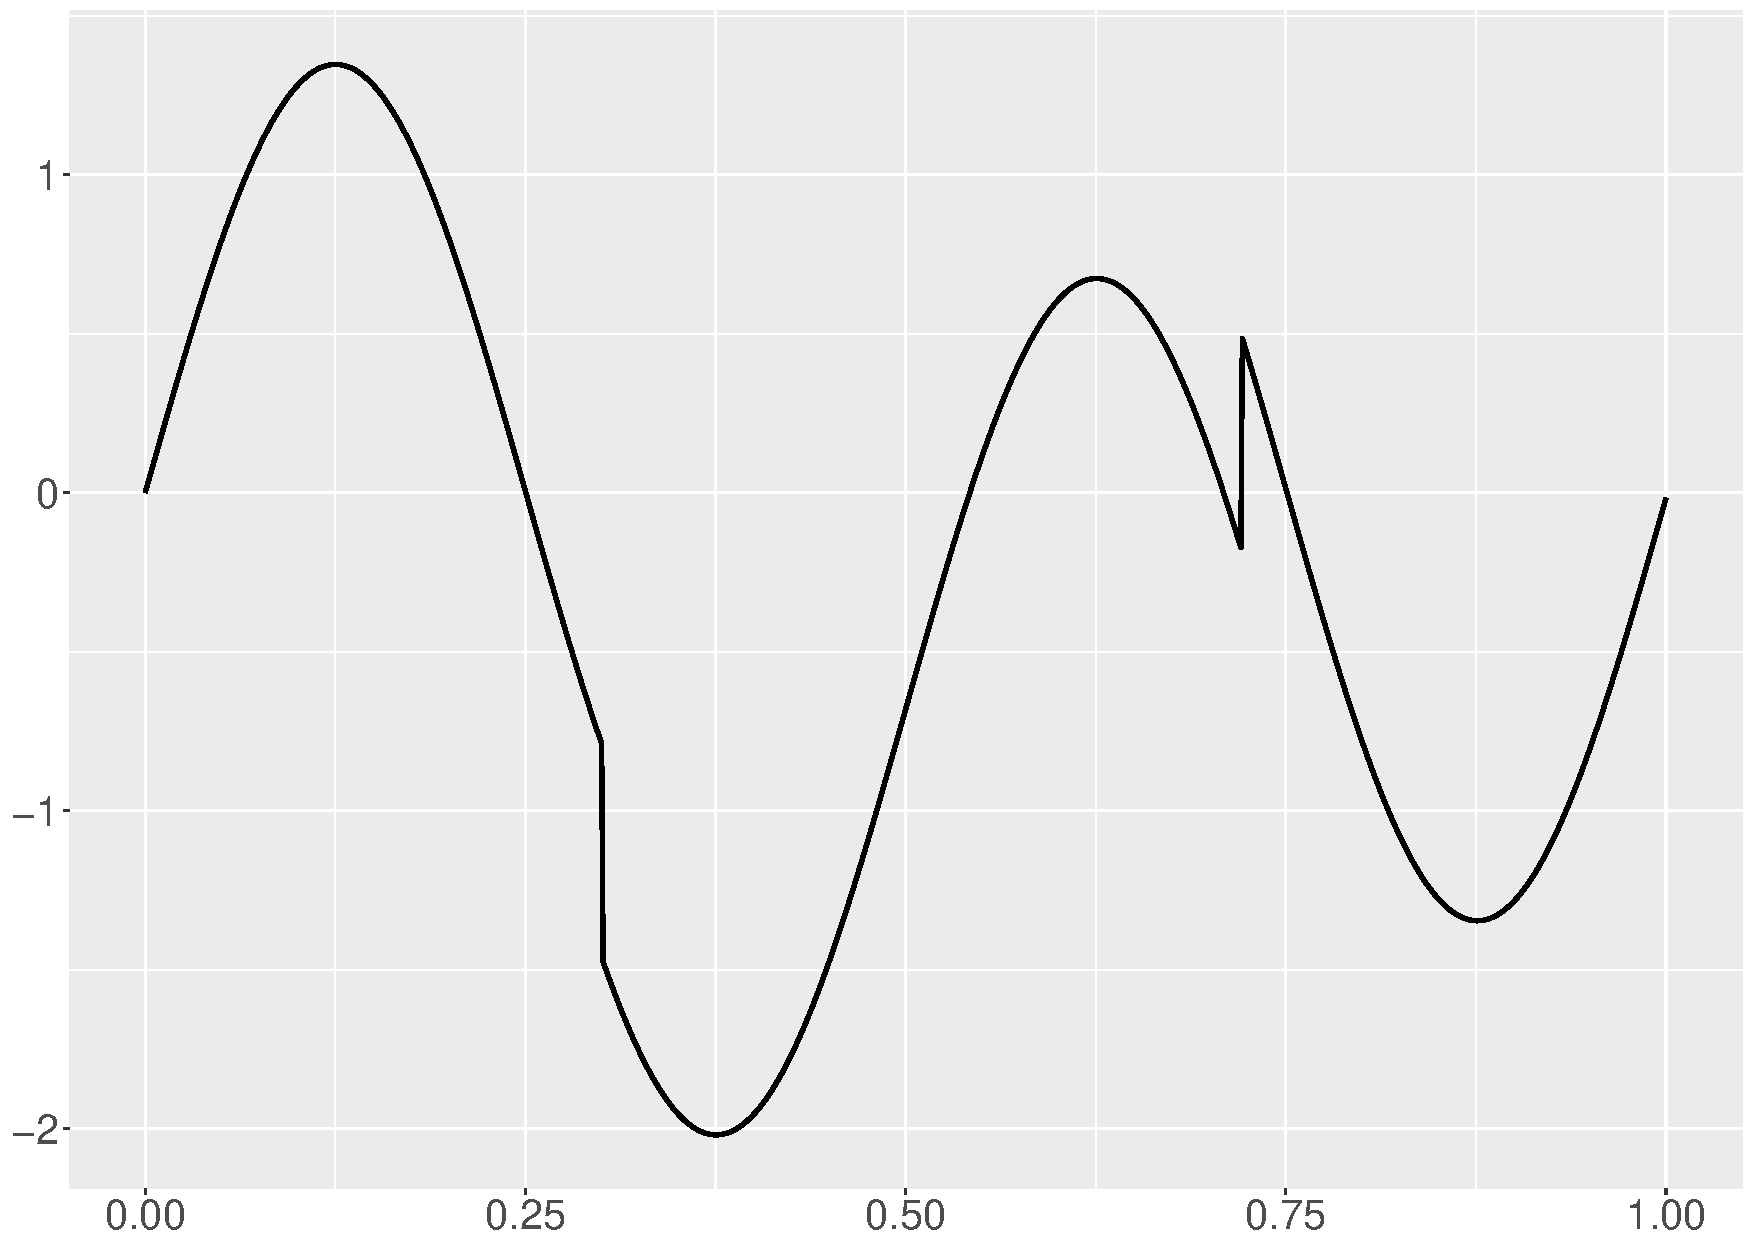
\includegraphics[width=\linewidth,height=0.45\textwidth]{Chapters/02TractorSplineTheory/plot/ggplot/ggHeaviSine.pdf}
    \caption{True \textit{HeaviSine} function.}
    \end{subfigure}%
    \begin{subfigure}{0.45\textwidth}
    \centering
    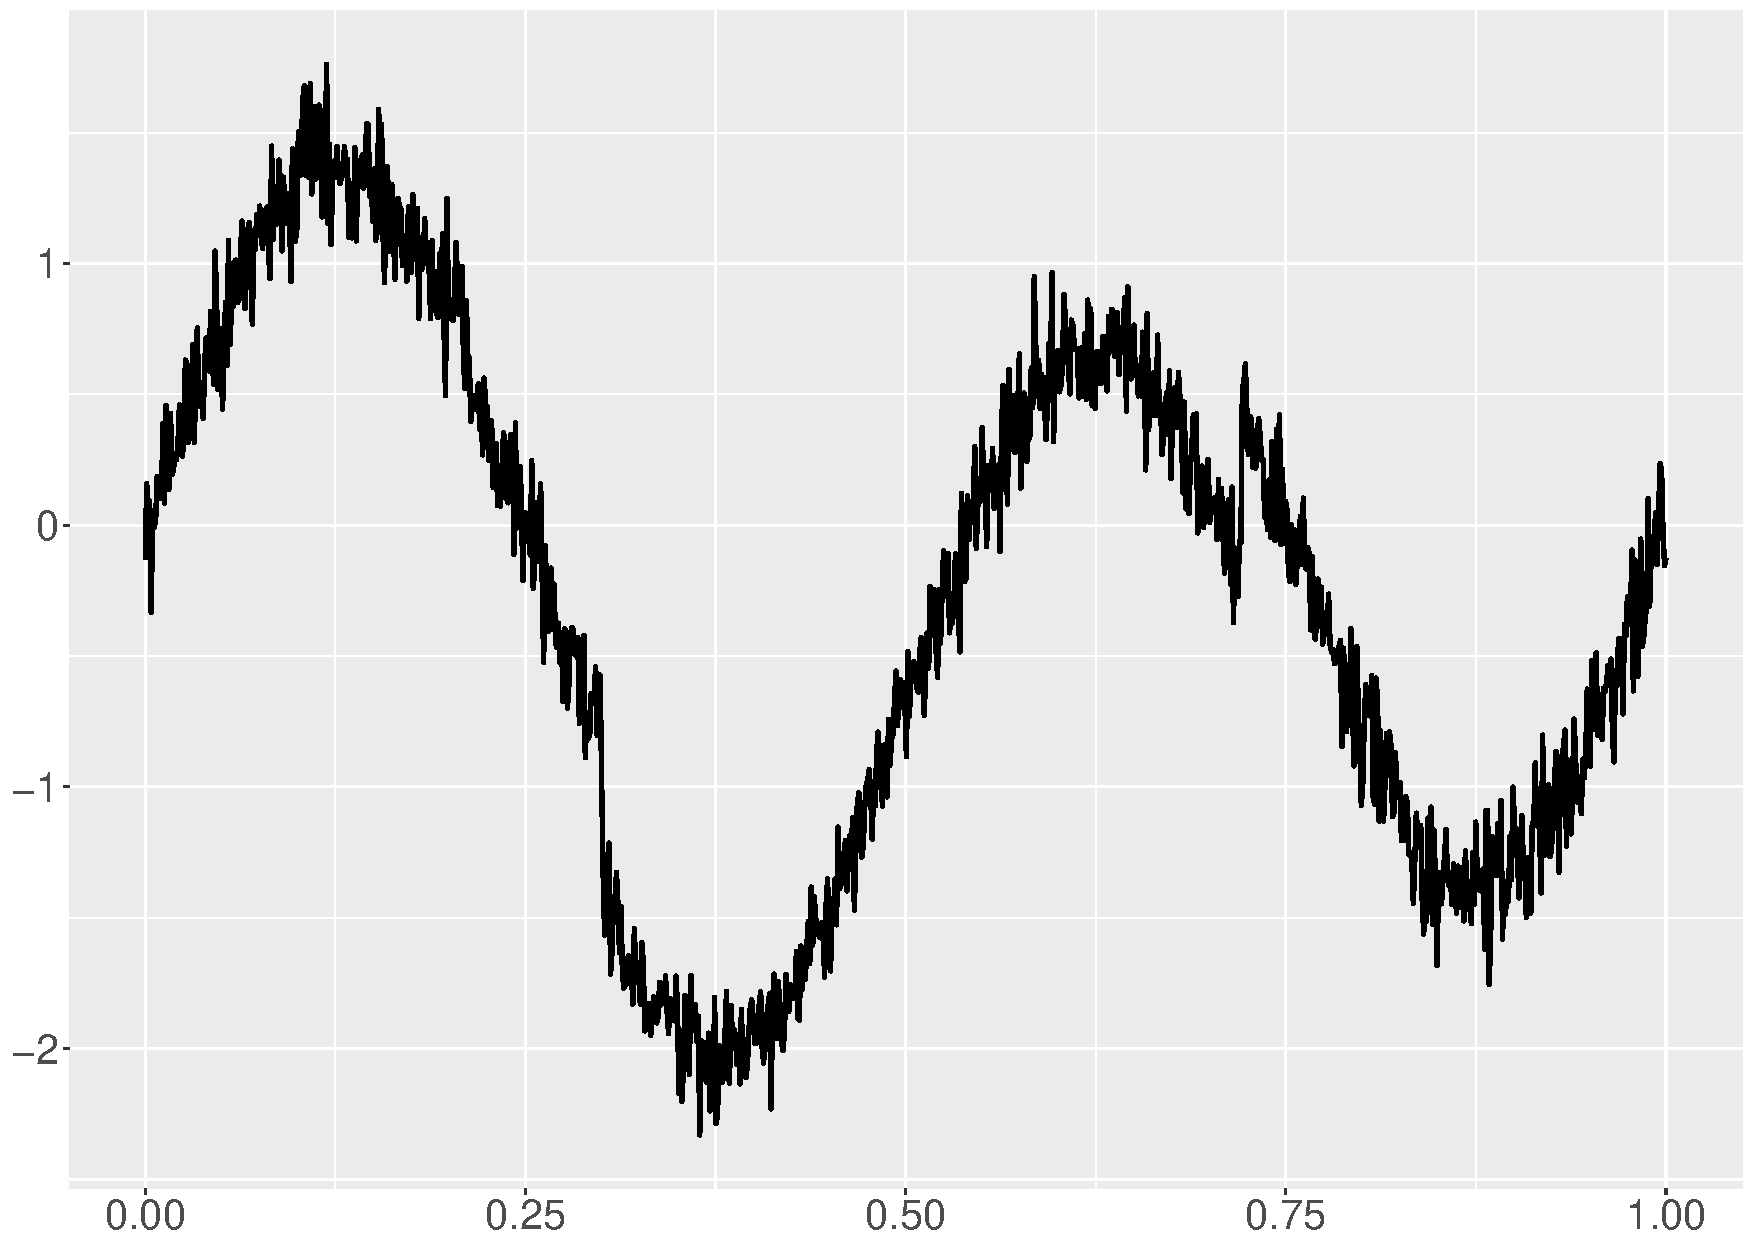
\includegraphics[width=\linewidth,,height=0.45\textwidth]{Chapters/02TractorSplineTheory/plot/ggplot/ggHeaviSineNoise.pdf}
    \caption{Noisy \textit{HeaviSine} at \textit{SNR}=7.}
    \end{subfigure}
    \begin{subfigure}{0.45\textwidth}
    \centering
    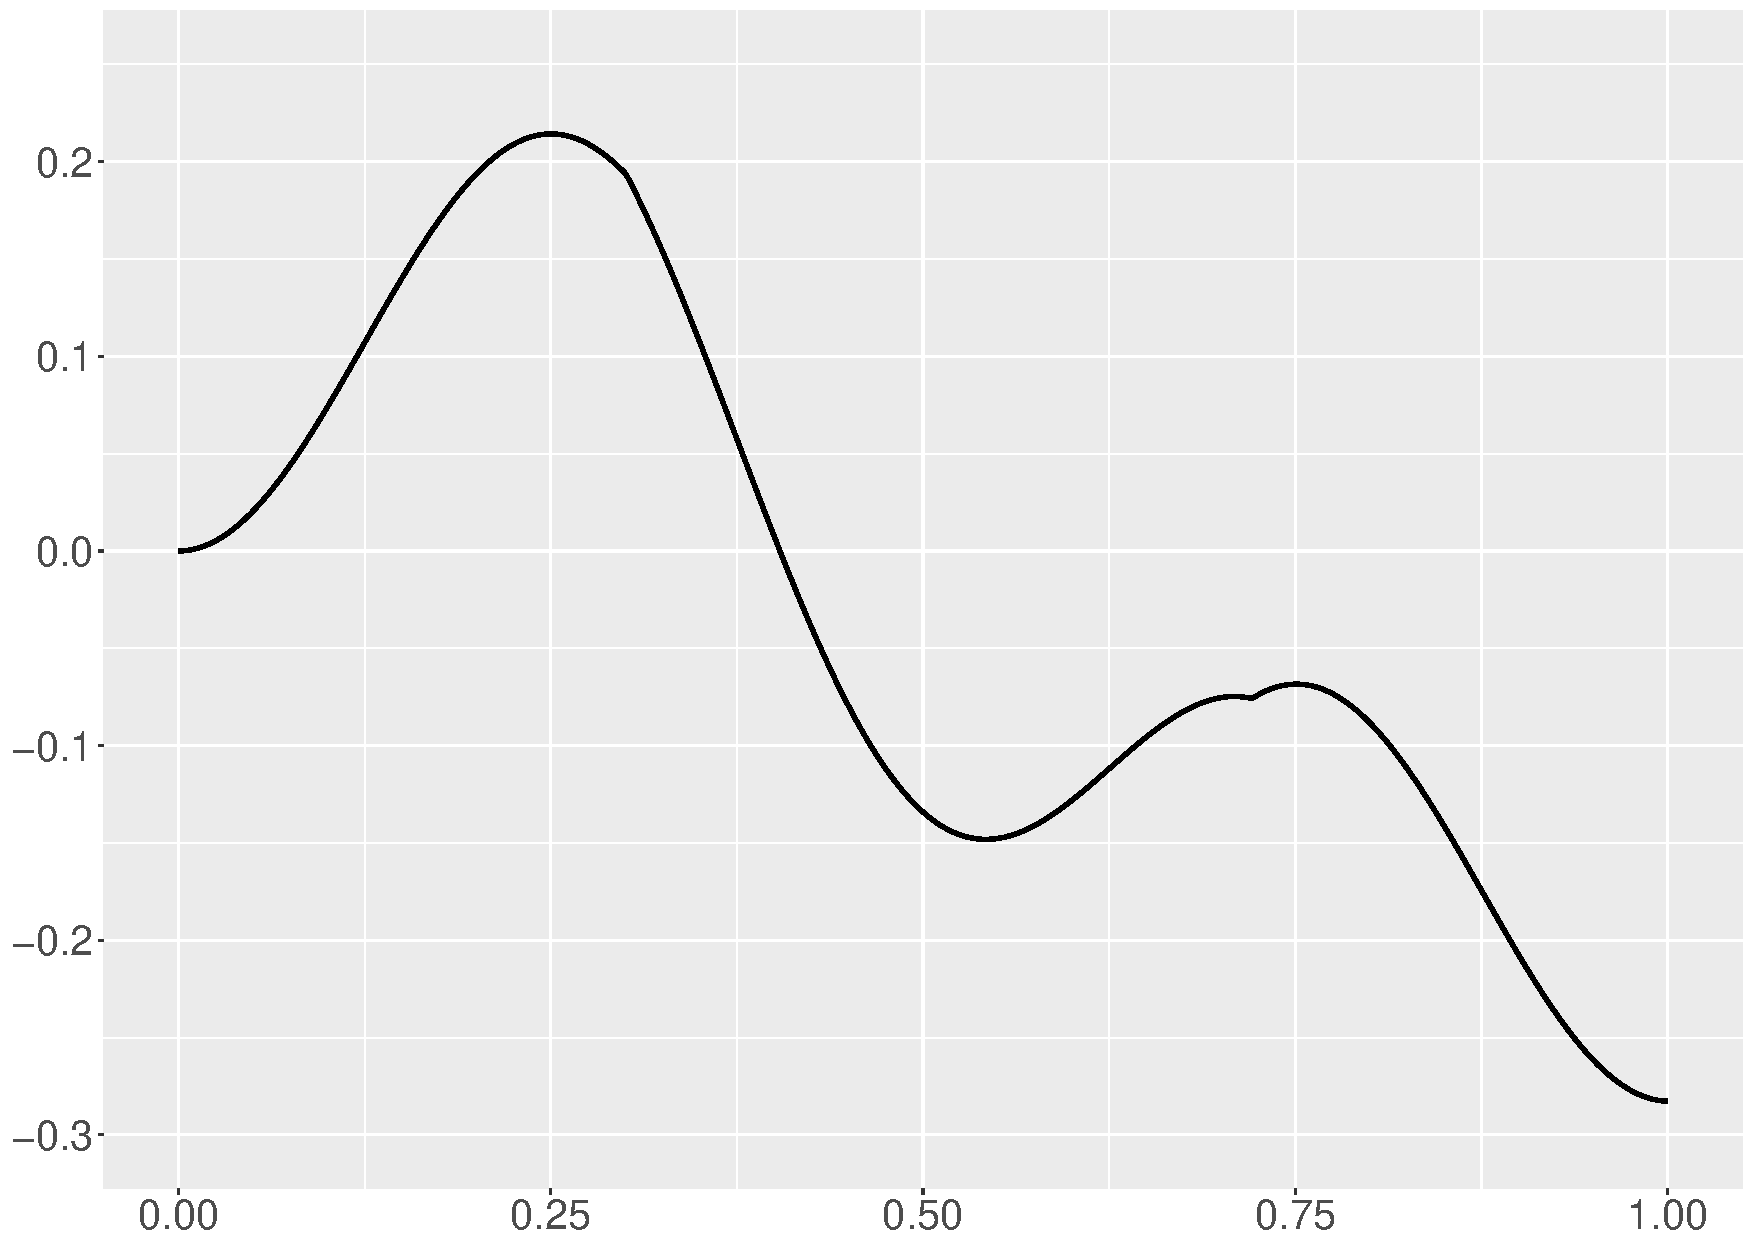
\includegraphics[width=\linewidth,height=0.45\textwidth]{Chapters/02TractorSplineTheory/plot/ggplot/ggHeaviSinePosition.pdf}
    \caption{Generated positions.}
    \end{subfigure}
    \begin{subfigure}{0.45\textwidth}
    \centering
    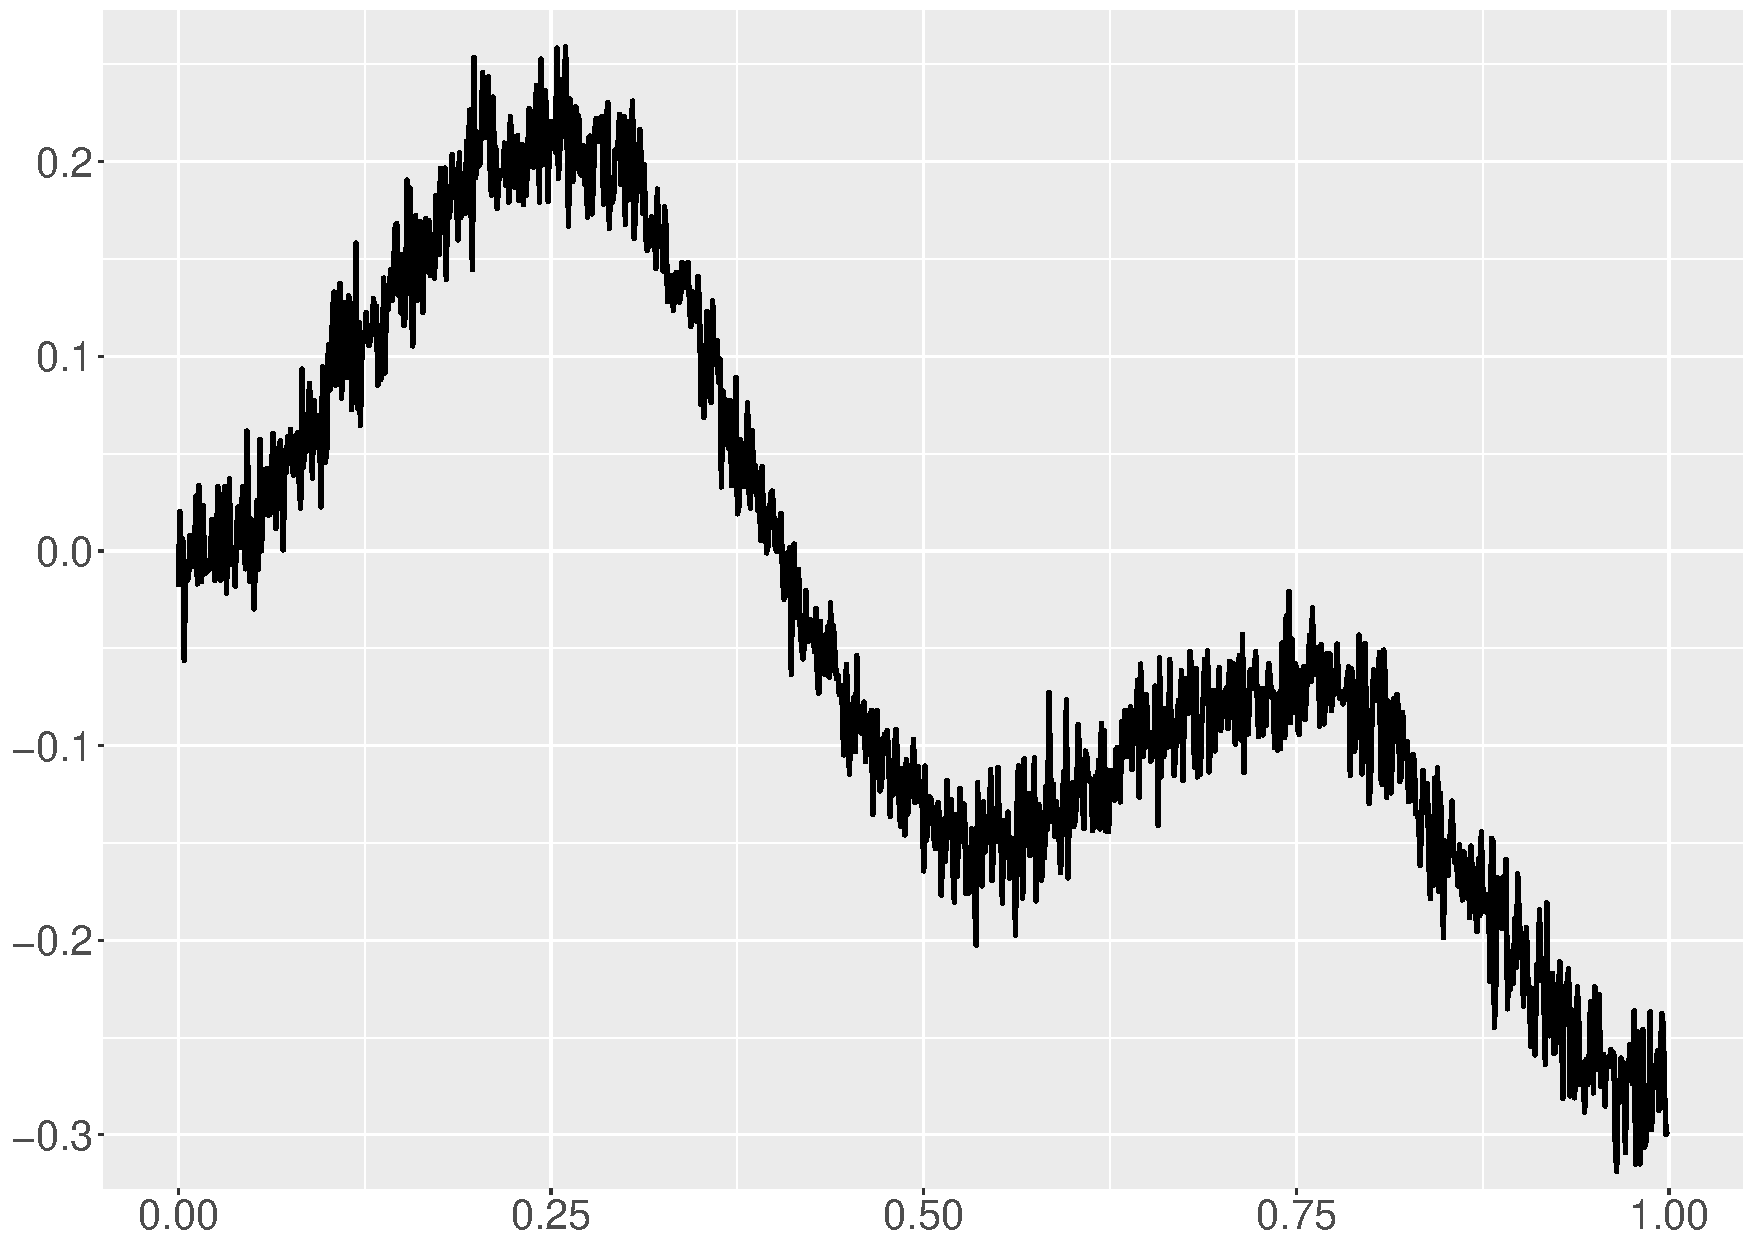
\includegraphics[width=\linewidth,height=0.45\textwidth]{Chapters/02TractorSplineTheory/plot/ggplot/ggHeaviSinePositionNoise.pdf}
    \caption{Noisy position at \textit{SNR}=7.}
    \end{subfigure}
    \begin{subfigure}{0.45\textwidth}
    \centering
    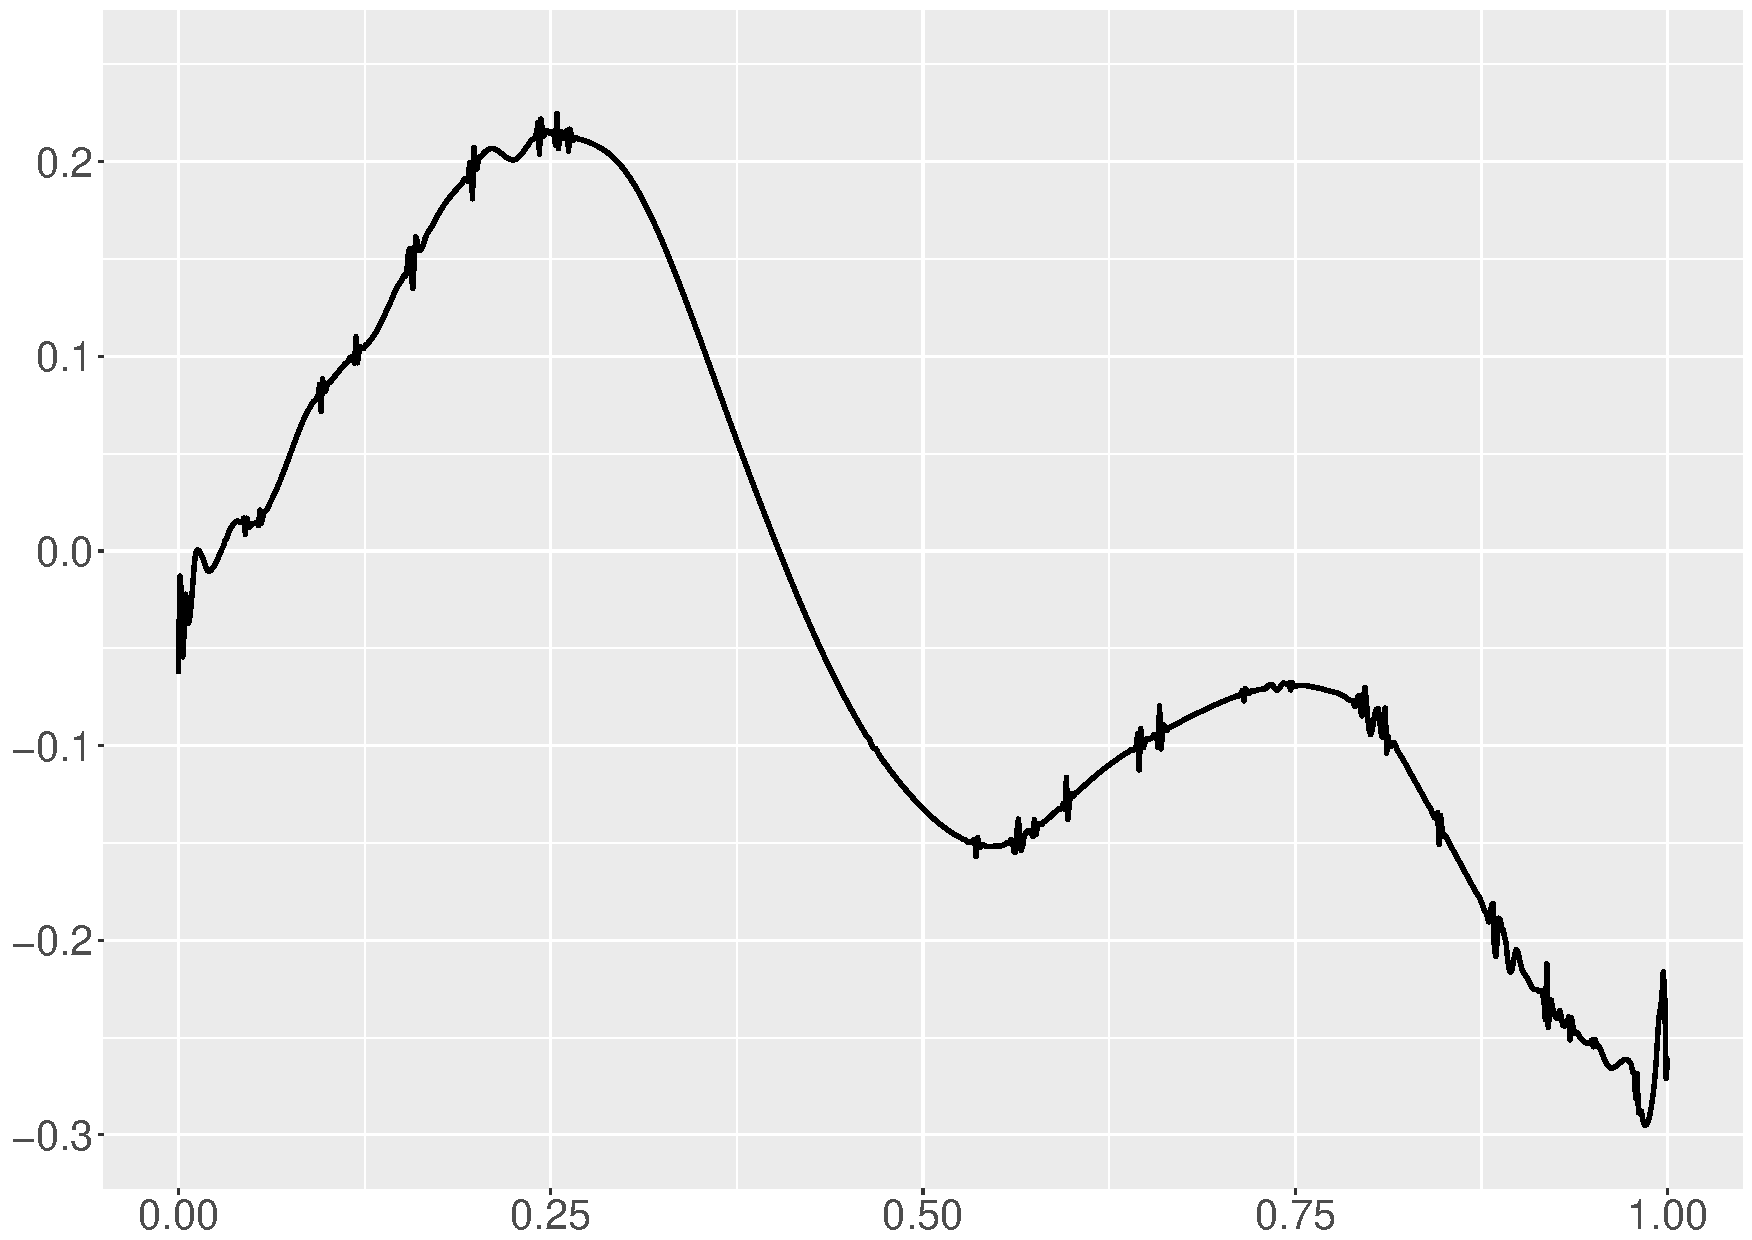
\includegraphics[width=\linewidth,height=0.45\textwidth]{Chapters/02TractorSplineTheory/plot/ggplot/ggHeaviSineSure.pdf}
    \caption{Reconstruction from Wavelet by sure threshold.}
    \end{subfigure}
    \begin{subfigure}{0.45\textwidth}
    \centering
    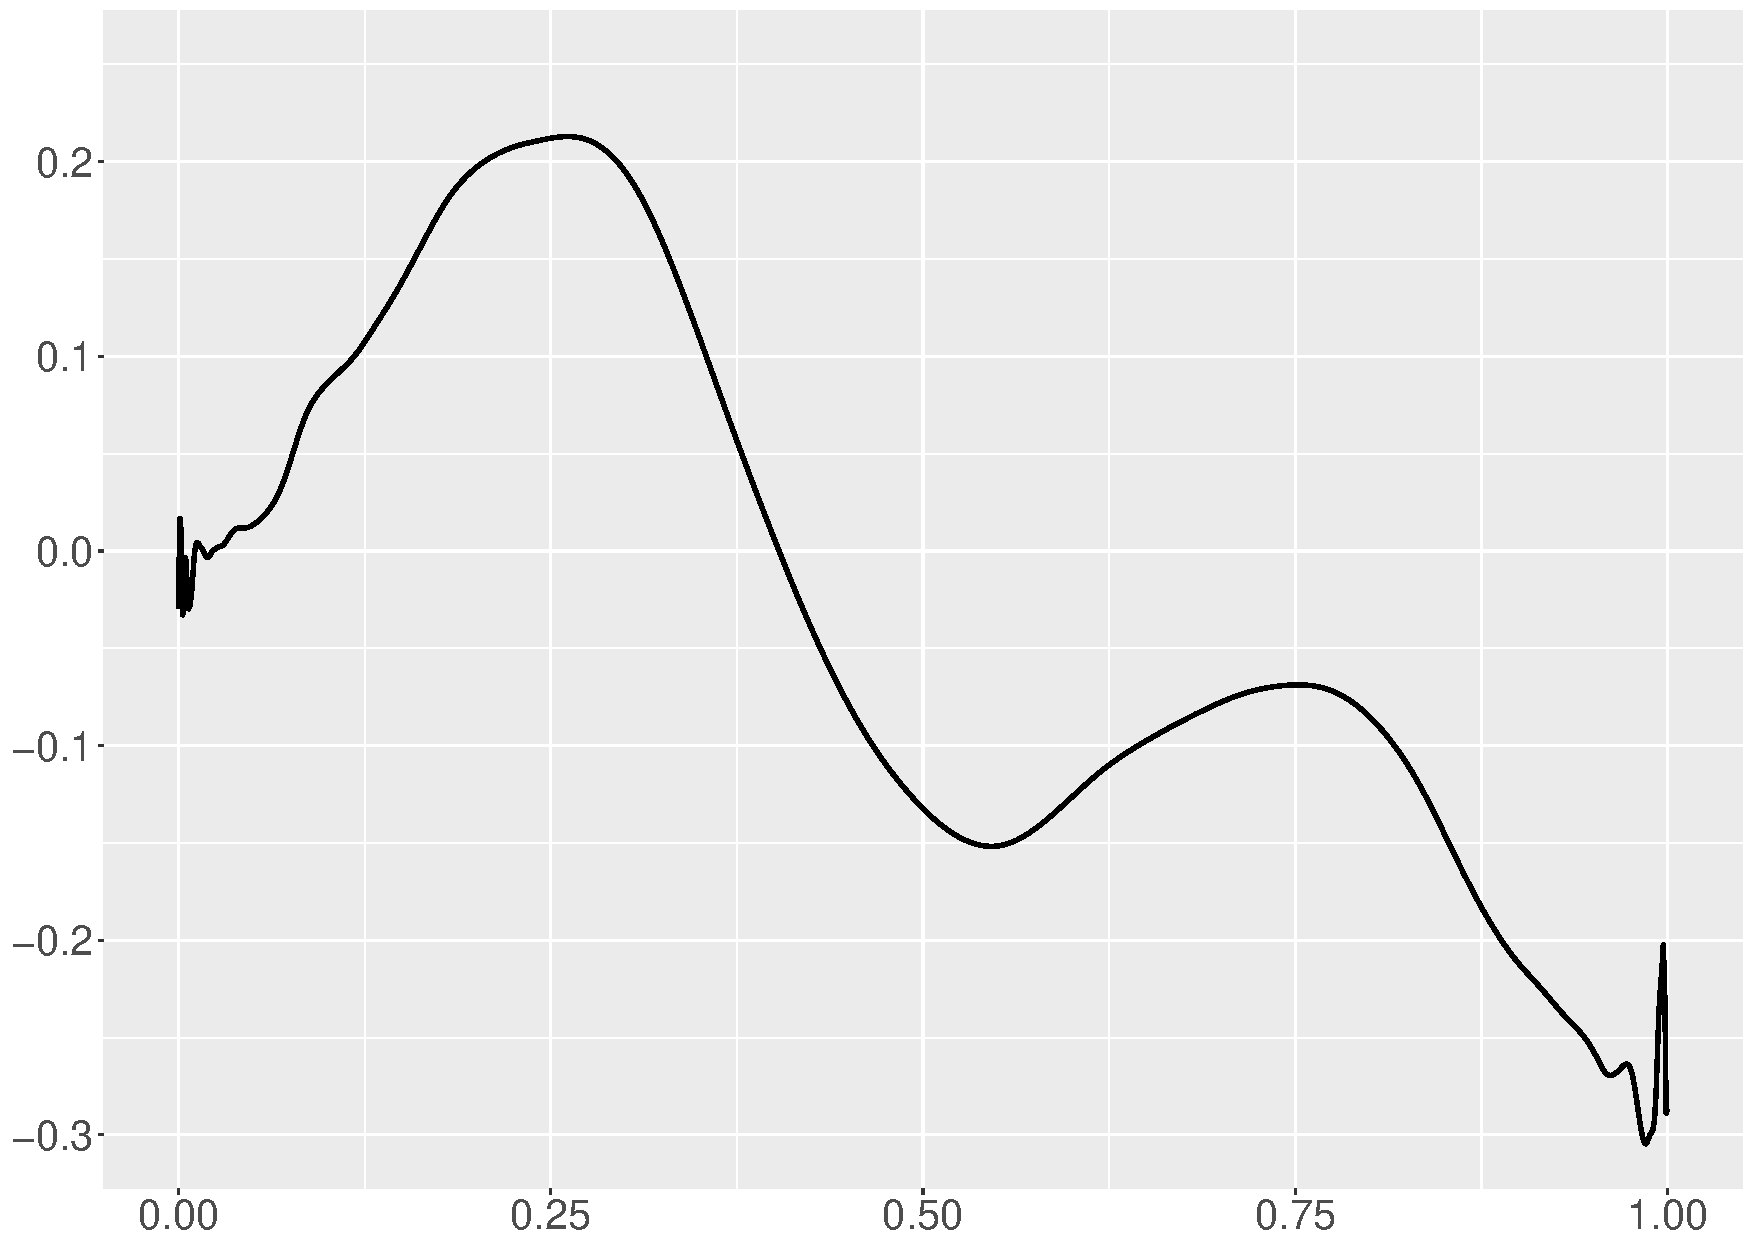
\includegraphics[width=\linewidth,height=0.45\textwidth]{Chapters/02TractorSplineTheory/plot/ggplot/ggHeaviSineBayes.pdf}
    \caption{Reconstruction from Wavelet by BayesThresh approach.}
    \end{subfigure}
    \begin{subfigure}{0.45\textwidth}
    \centering
    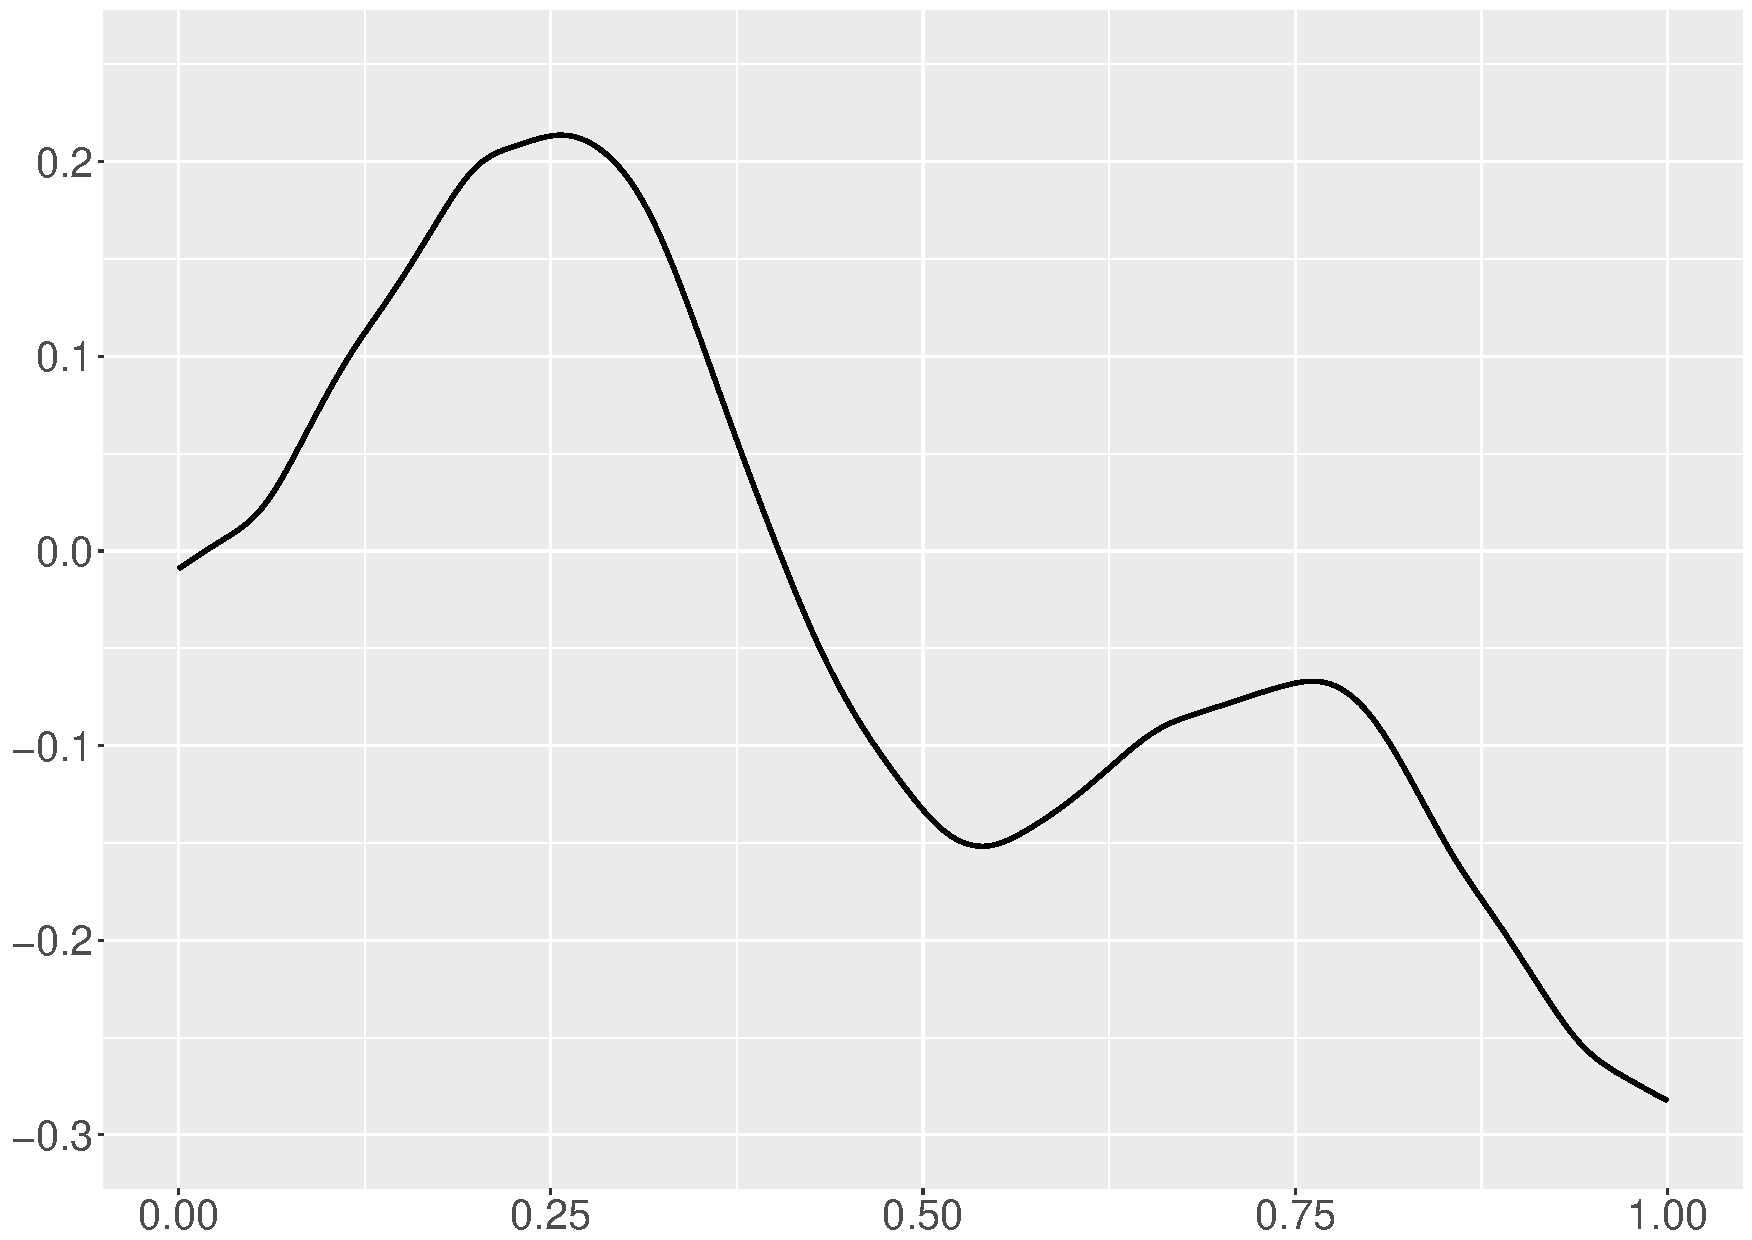
\includegraphics[width=\linewidth,height=0.45\textwidth]{Chapters/02TractorSplineTheory/plot/ggplot/ggHeaviSinePSpline.pdf}
    \caption{Reconstruction by P-spline. \\\mbox{  } }
    \end{subfigure}
    \begin{subfigure}{0.45\textwidth}
    \centering
    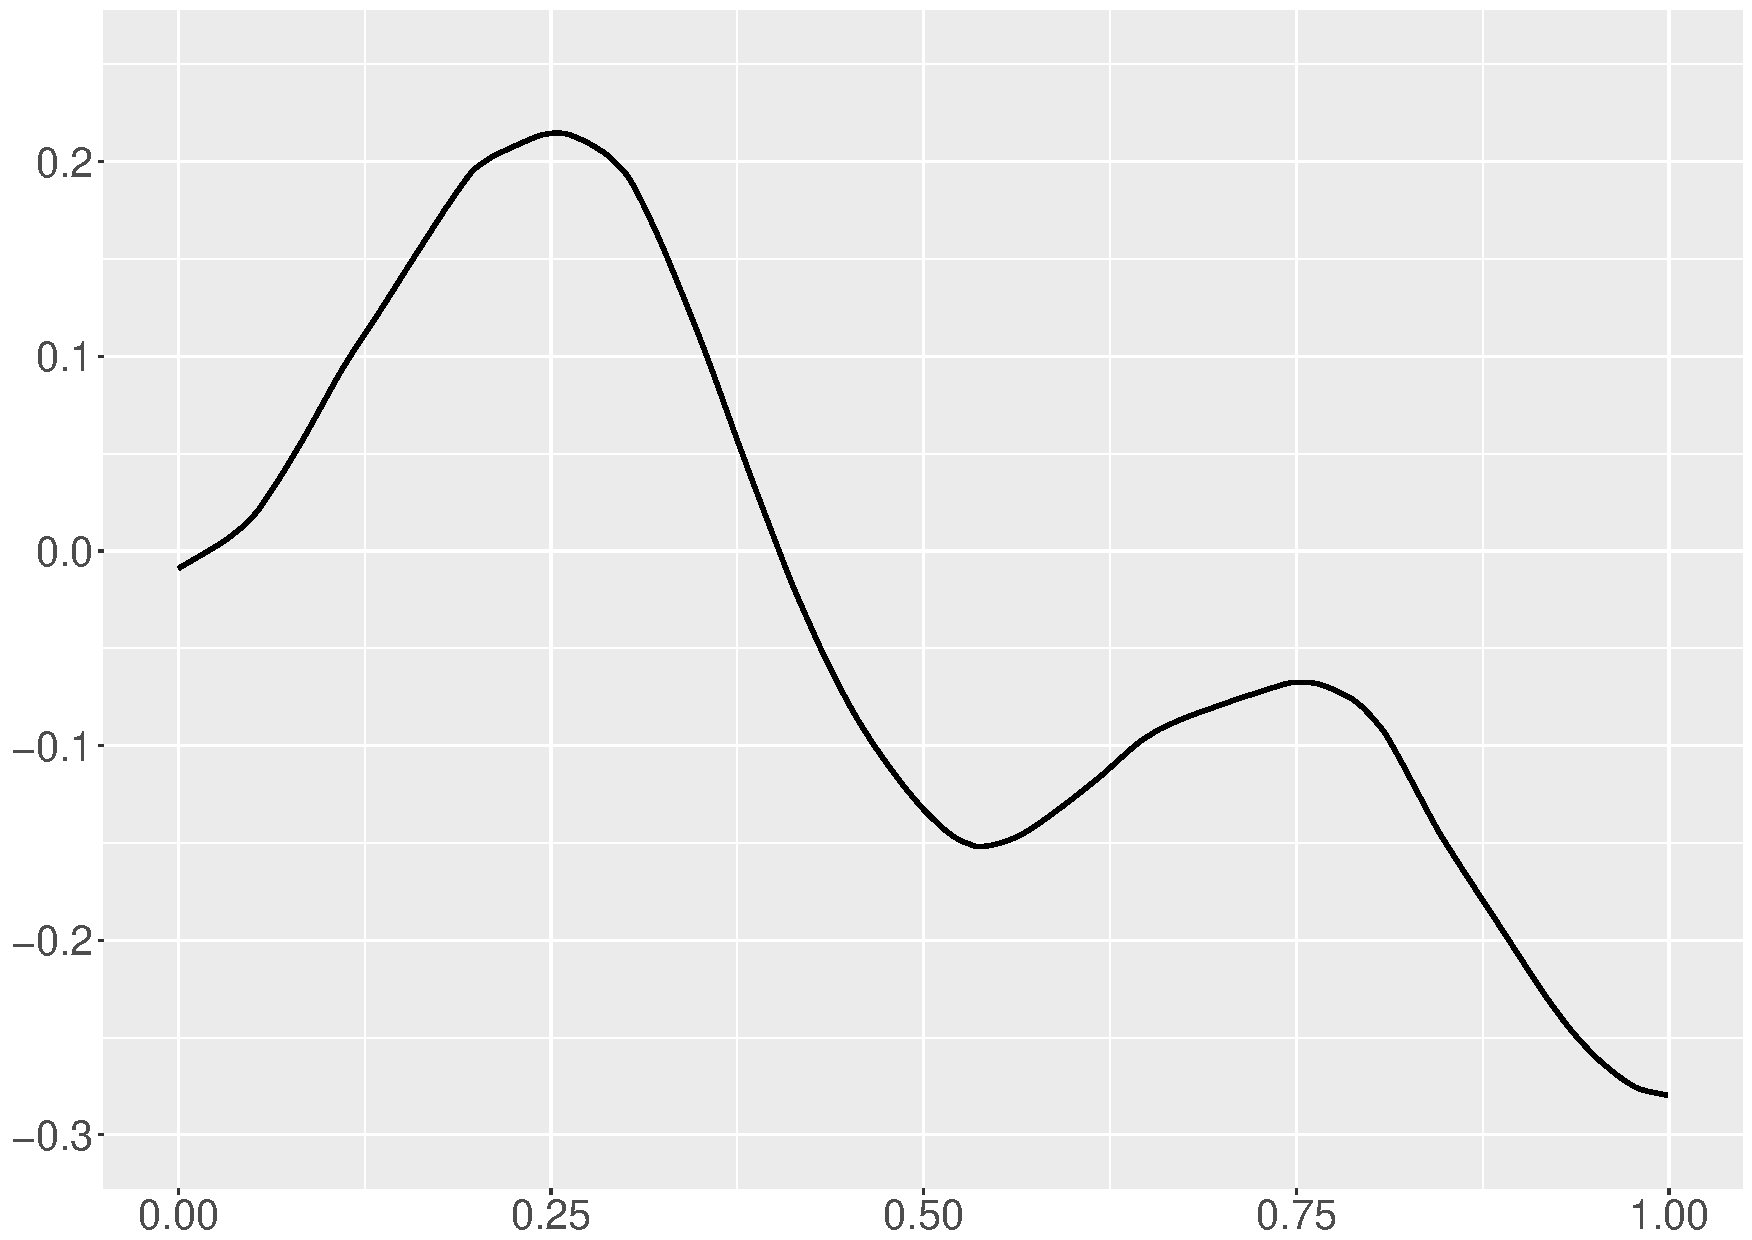
\includegraphics[width=\linewidth,height=0.45\textwidth]{Chapters/02TractorSplineTheory/plot/ggplot/ggHeaviSineGamma.pdf}
    \caption{Reconstruction by Tractor Spline setting $\gamma=0$}
    \end{subfigure}
  \begin{subfigure}{0.45\textwidth}
    \centering
    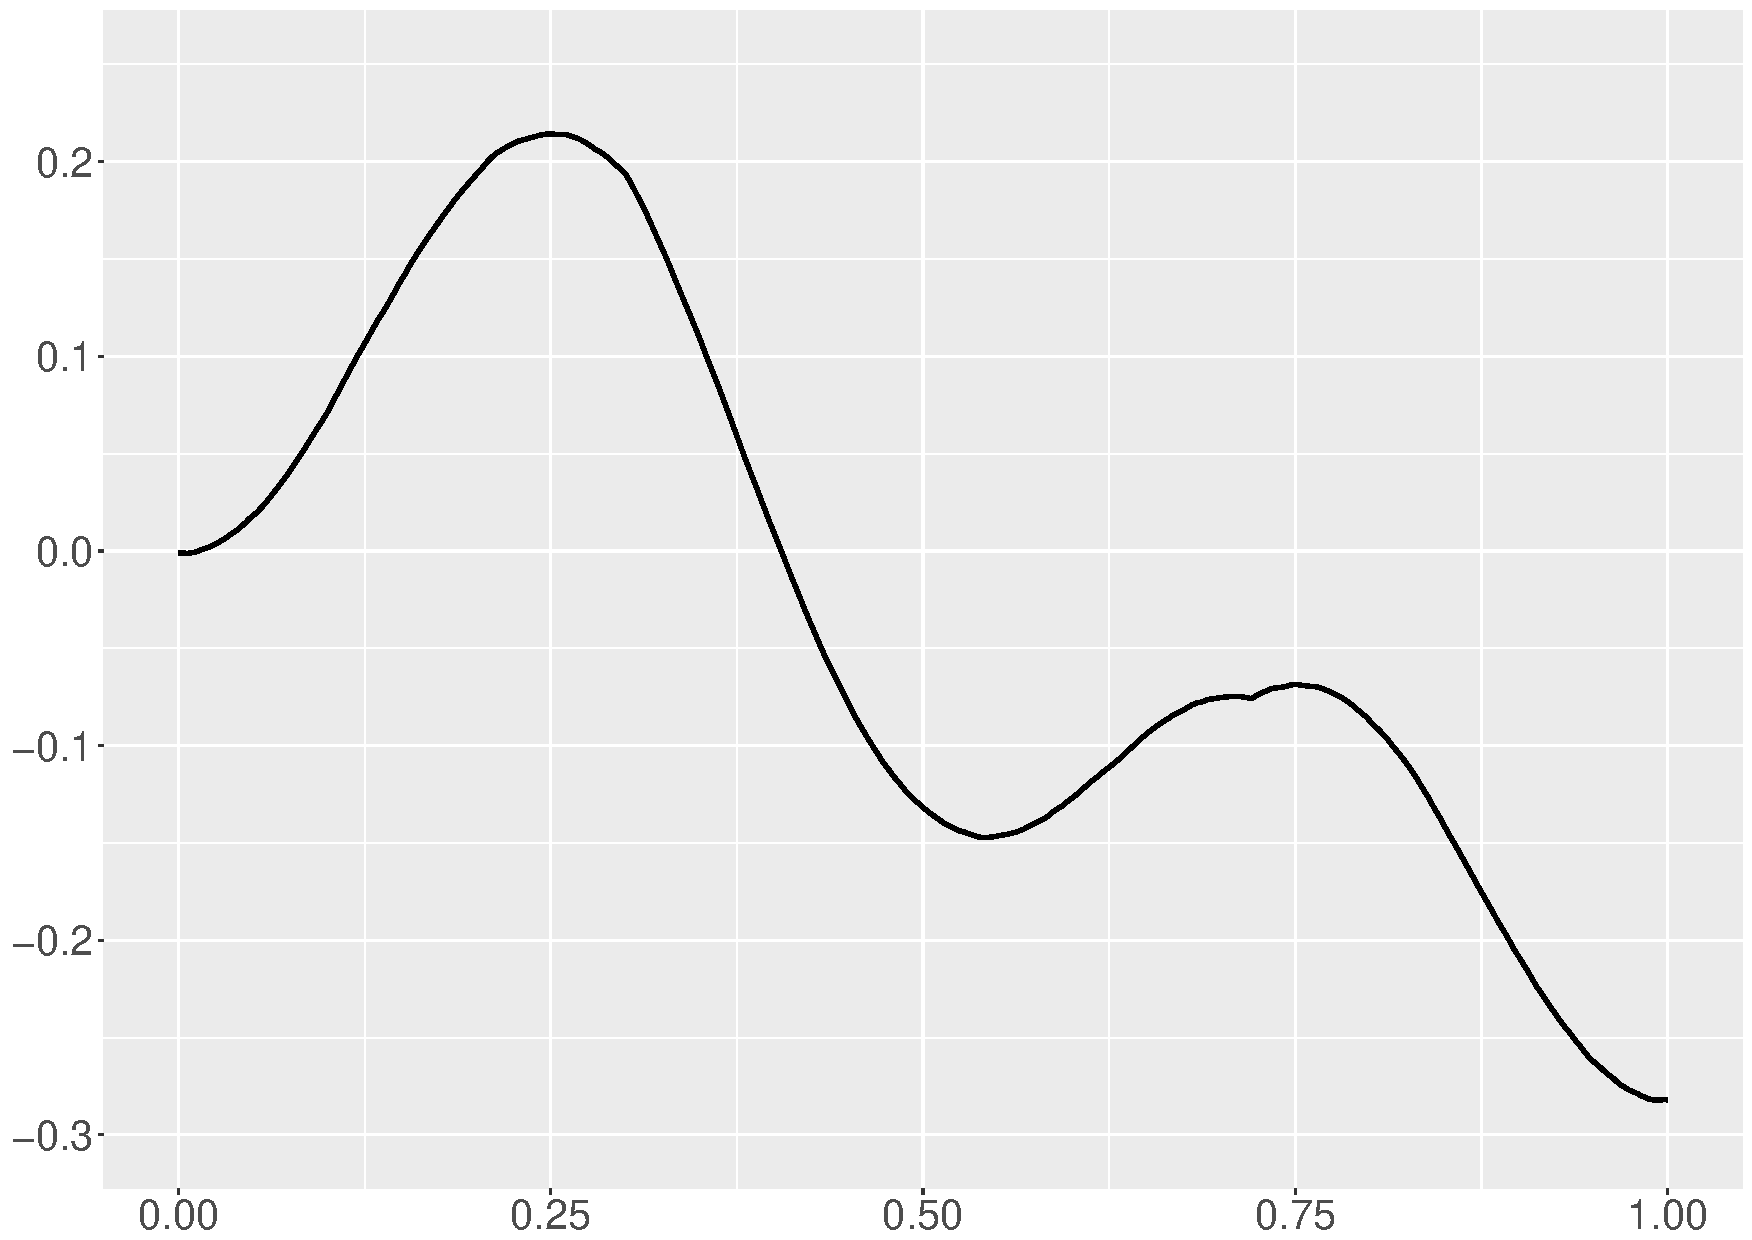
\includegraphics[width=\linewidth,height=0.45\textwidth]{Chapters/02TractorSplineTheory/plot/ggplot/ggHeaviSineTractorAPT.pdf}
    \caption{Reconstruction by Tractor Spline with conventional penalty term.}
    \end{subfigure}
    \begin{subfigure}{0.45\textwidth}
    \centering
    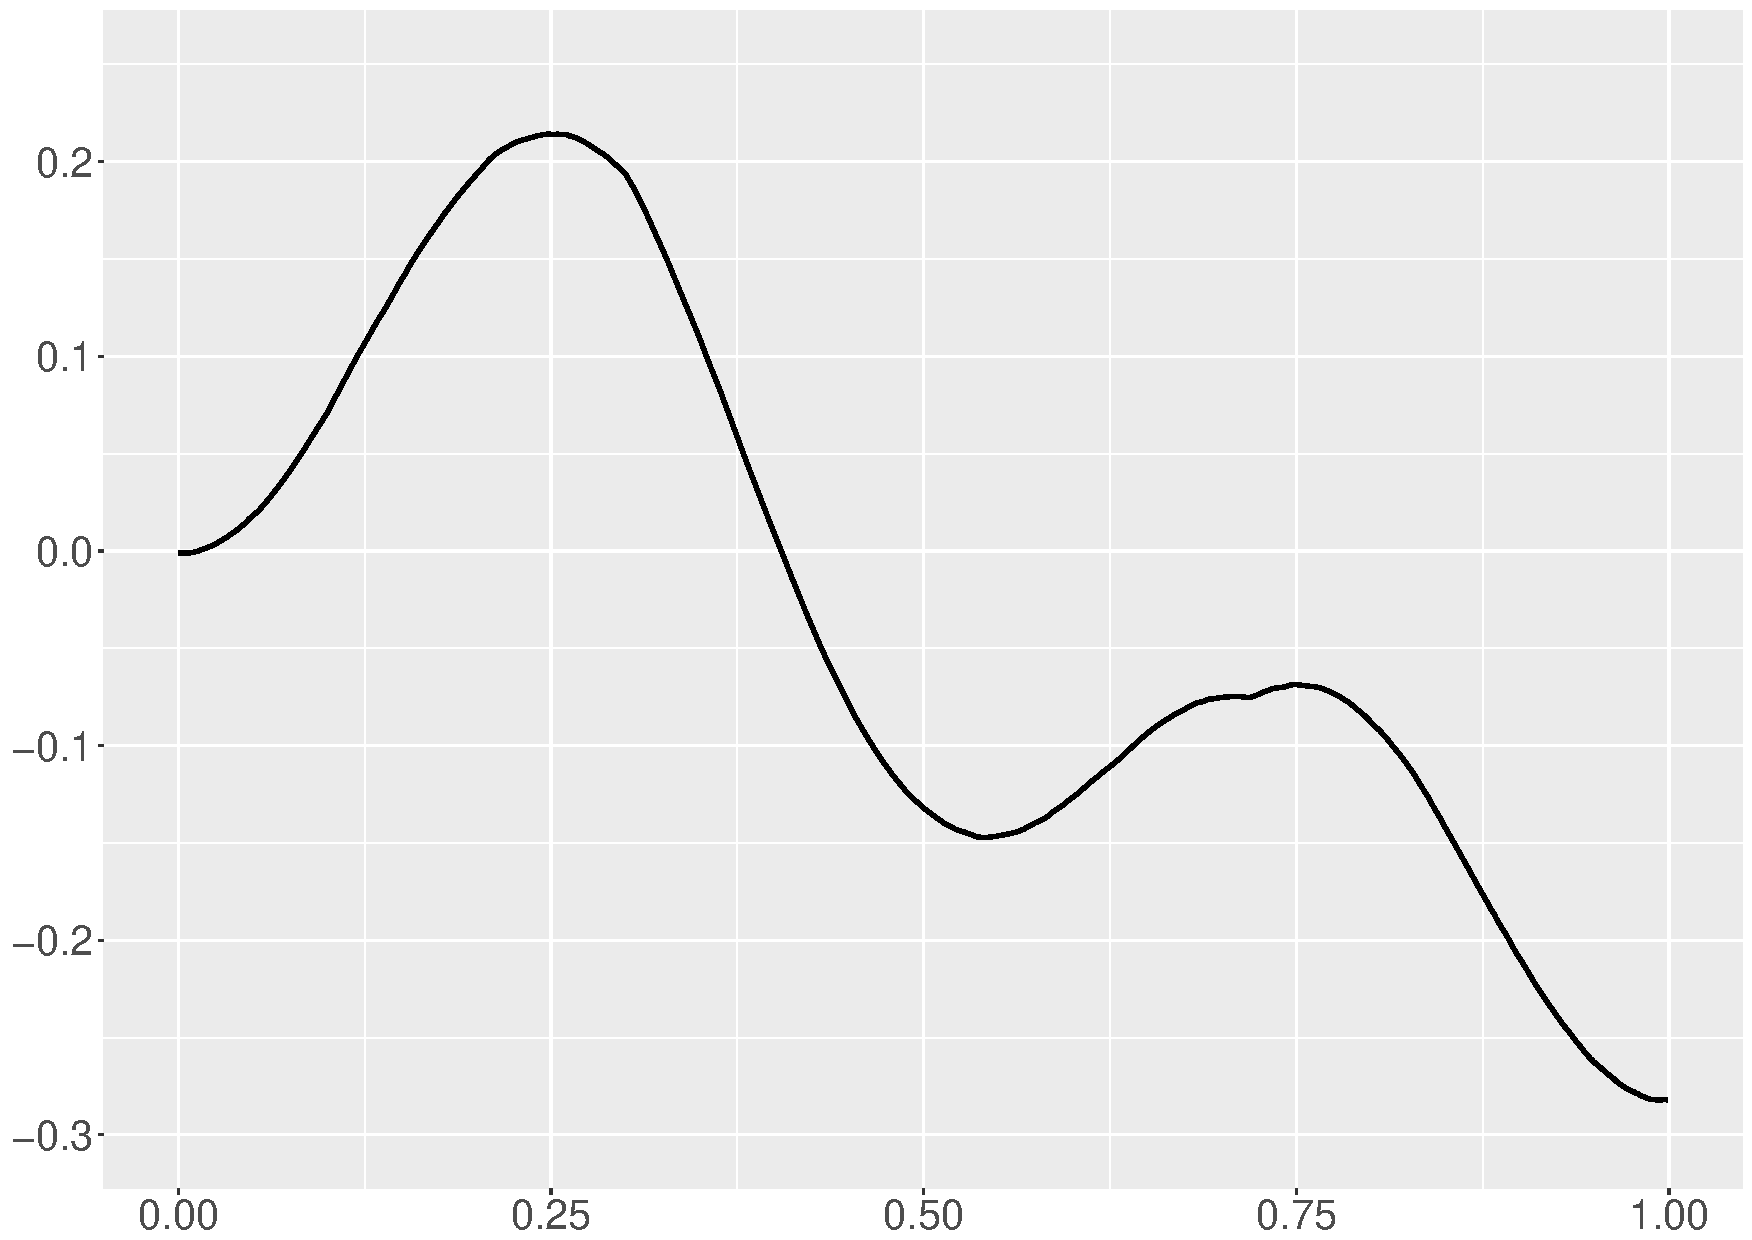
\includegraphics[width=\linewidth,height=0.45\textwidth]{Chapters/02TractorSplineTheory/plot/ggplot/ggHeaviSineTractor.pdf}
    \caption{Reconstruction by proposed Tractor Spline.}
    \end{subfigure}
\caption{Numerical example: $\textit{HeaviSine}$. Comparison of different reconstruction methods with simulated data.}\label{num3}
 \end{figure}

%
%
%\begin{figure}
%  \centering
%         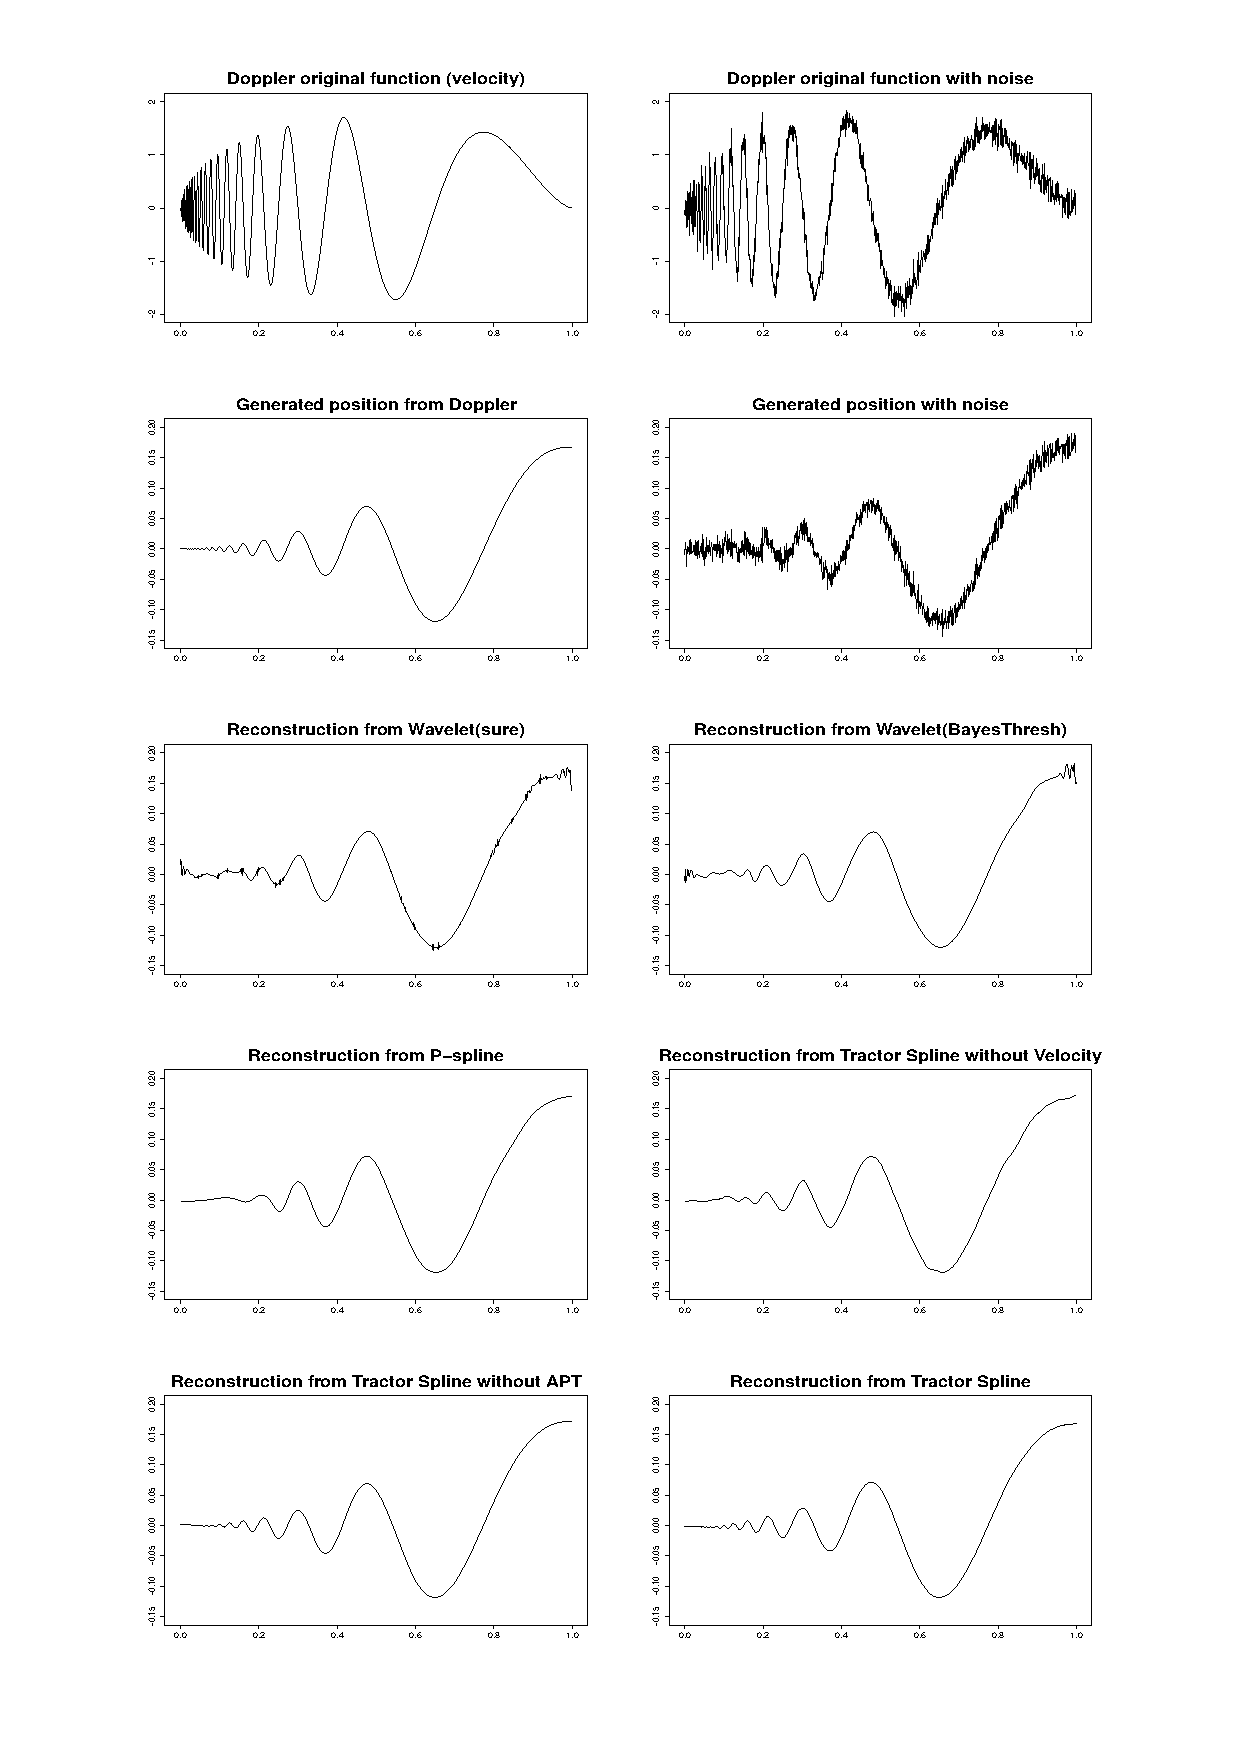
\includegraphics[width=\textwidth,height=14cm]{Chapters/02TractorSplineTheory/plot/doppler10} 
%  \caption{Numerical example: $\textit{Doppler}$. (a) The true velocity function. (b) Velocity with Gaussian noise at SNR=7. (c) Generated position function. (d) Position with Gaussian noise at SNR=7. (e) Reconstruction from Wavelet with sure threshold. (f) Reconstruction from Wavelet with BayesThresh approach. (g) Reconstruction by P-spline. (h) Reconstruction by Tractor Spline setting $\gamma=0$. (i) Reconstruction by Tractor Spline with normal penalty term. (j) Reconstruction by proposed Tractor Spline.}\label{num4}
%\end{figure}


\begin{figure}
    \centering
    \begin{subfigure}{0.45\textwidth}
    \centering
    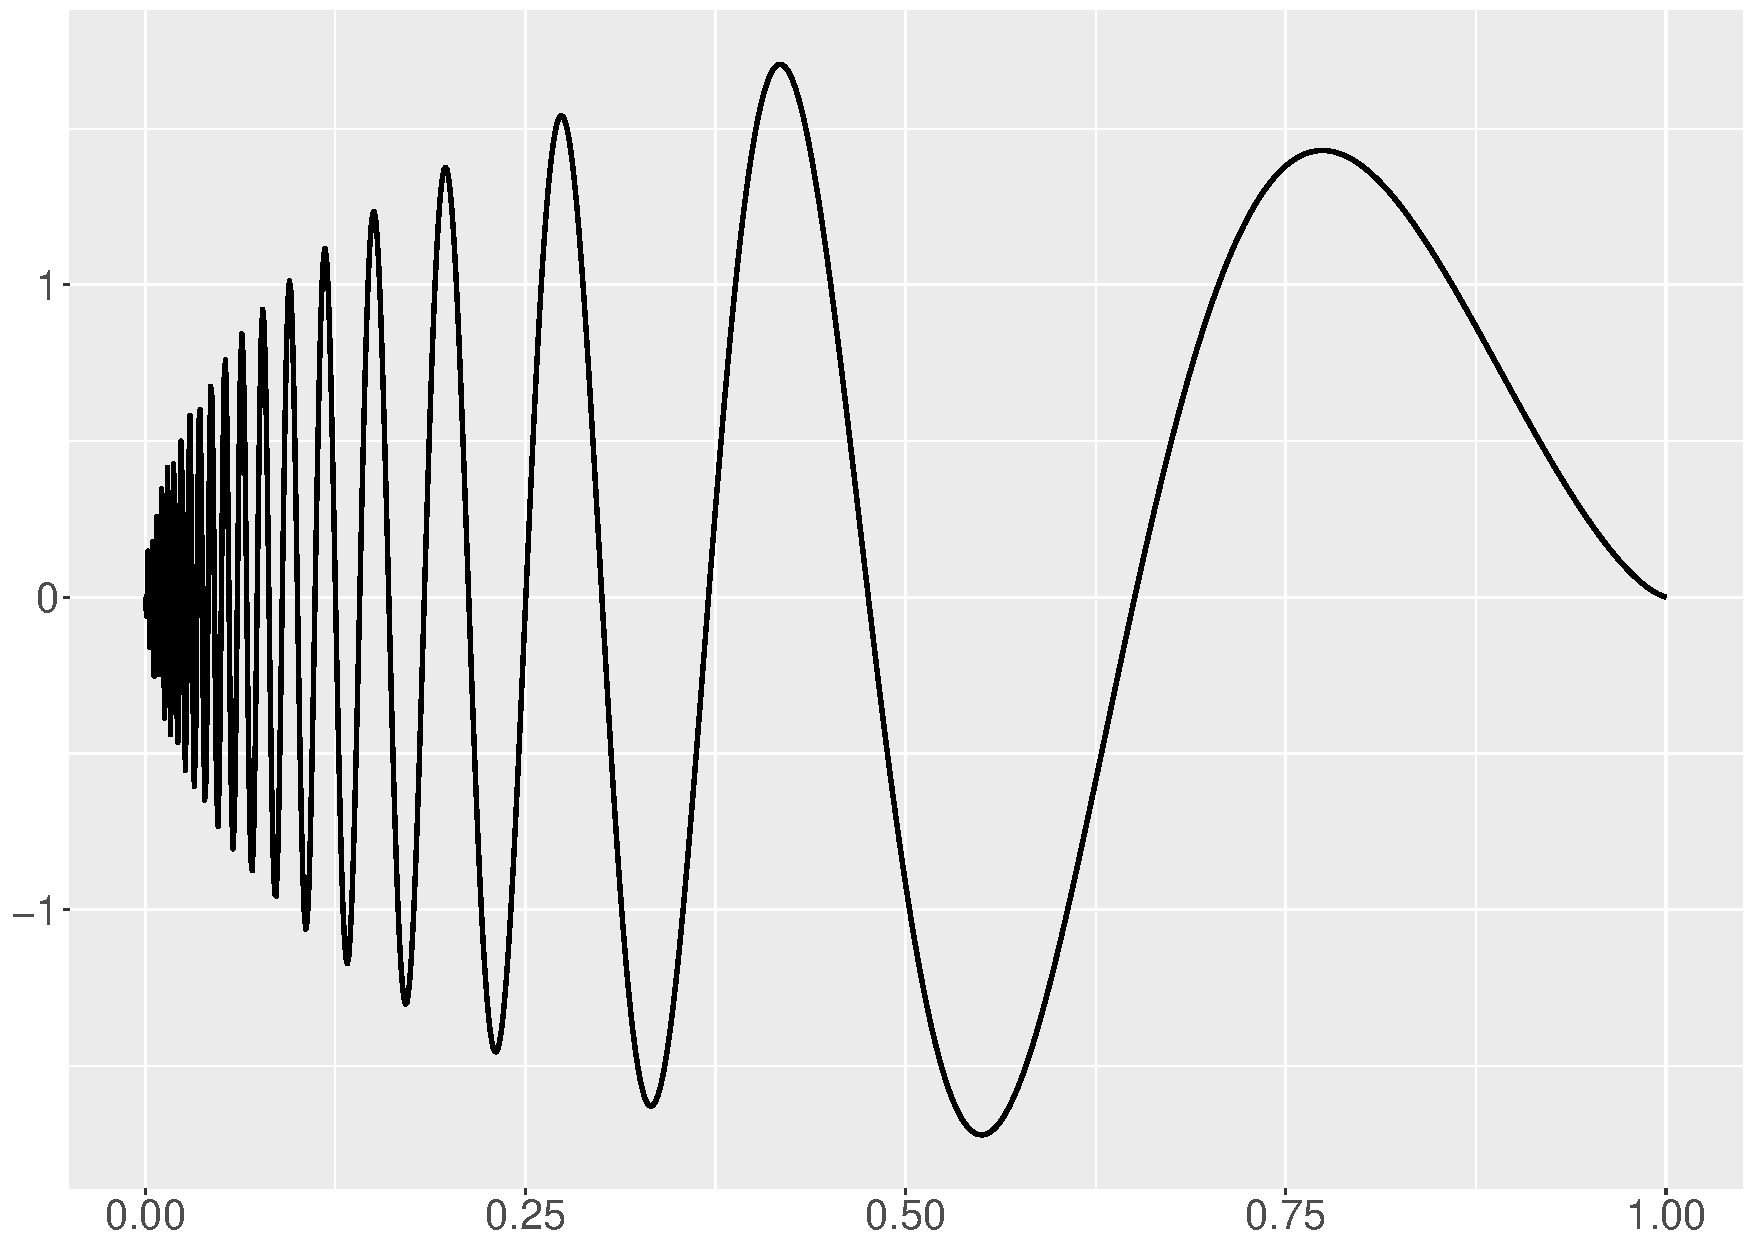
\includegraphics[width=\linewidth,height=0.45\textwidth]{Chapters/02TractorSplineTheory/plot/ggplot/ggDoppler.pdf}
    \caption{True \textit{Doppler} function.}
    \end{subfigure}%
    \begin{subfigure}{0.45\textwidth}
    \centering
    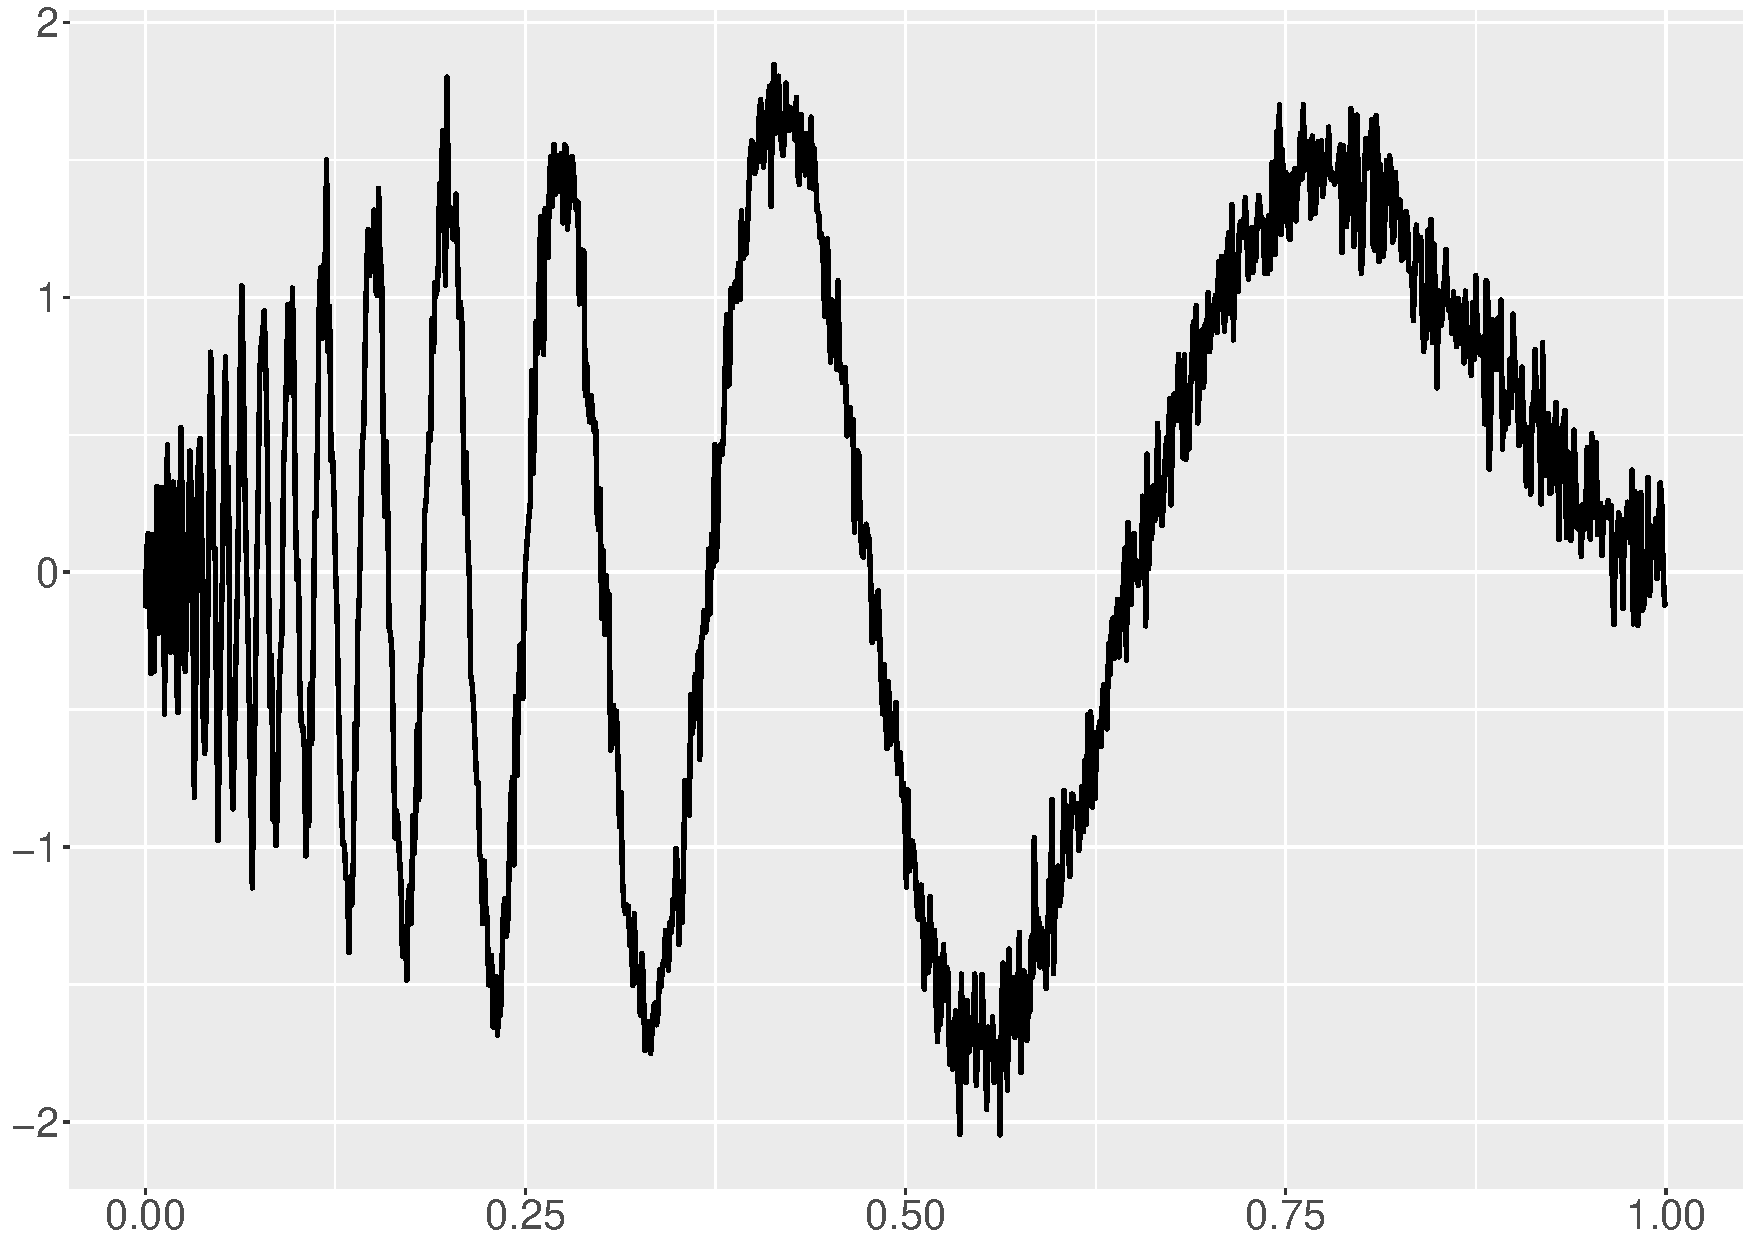
\includegraphics[width=\linewidth,,height=0.45\textwidth]{Chapters/02TractorSplineTheory/plot/ggplot/ggDopplerNoise.pdf}
    \caption{Noisy \textit{Doppler} at \textit{SNR}=7.}
    \end{subfigure}
    \begin{subfigure}{0.45\textwidth}
    \centering
    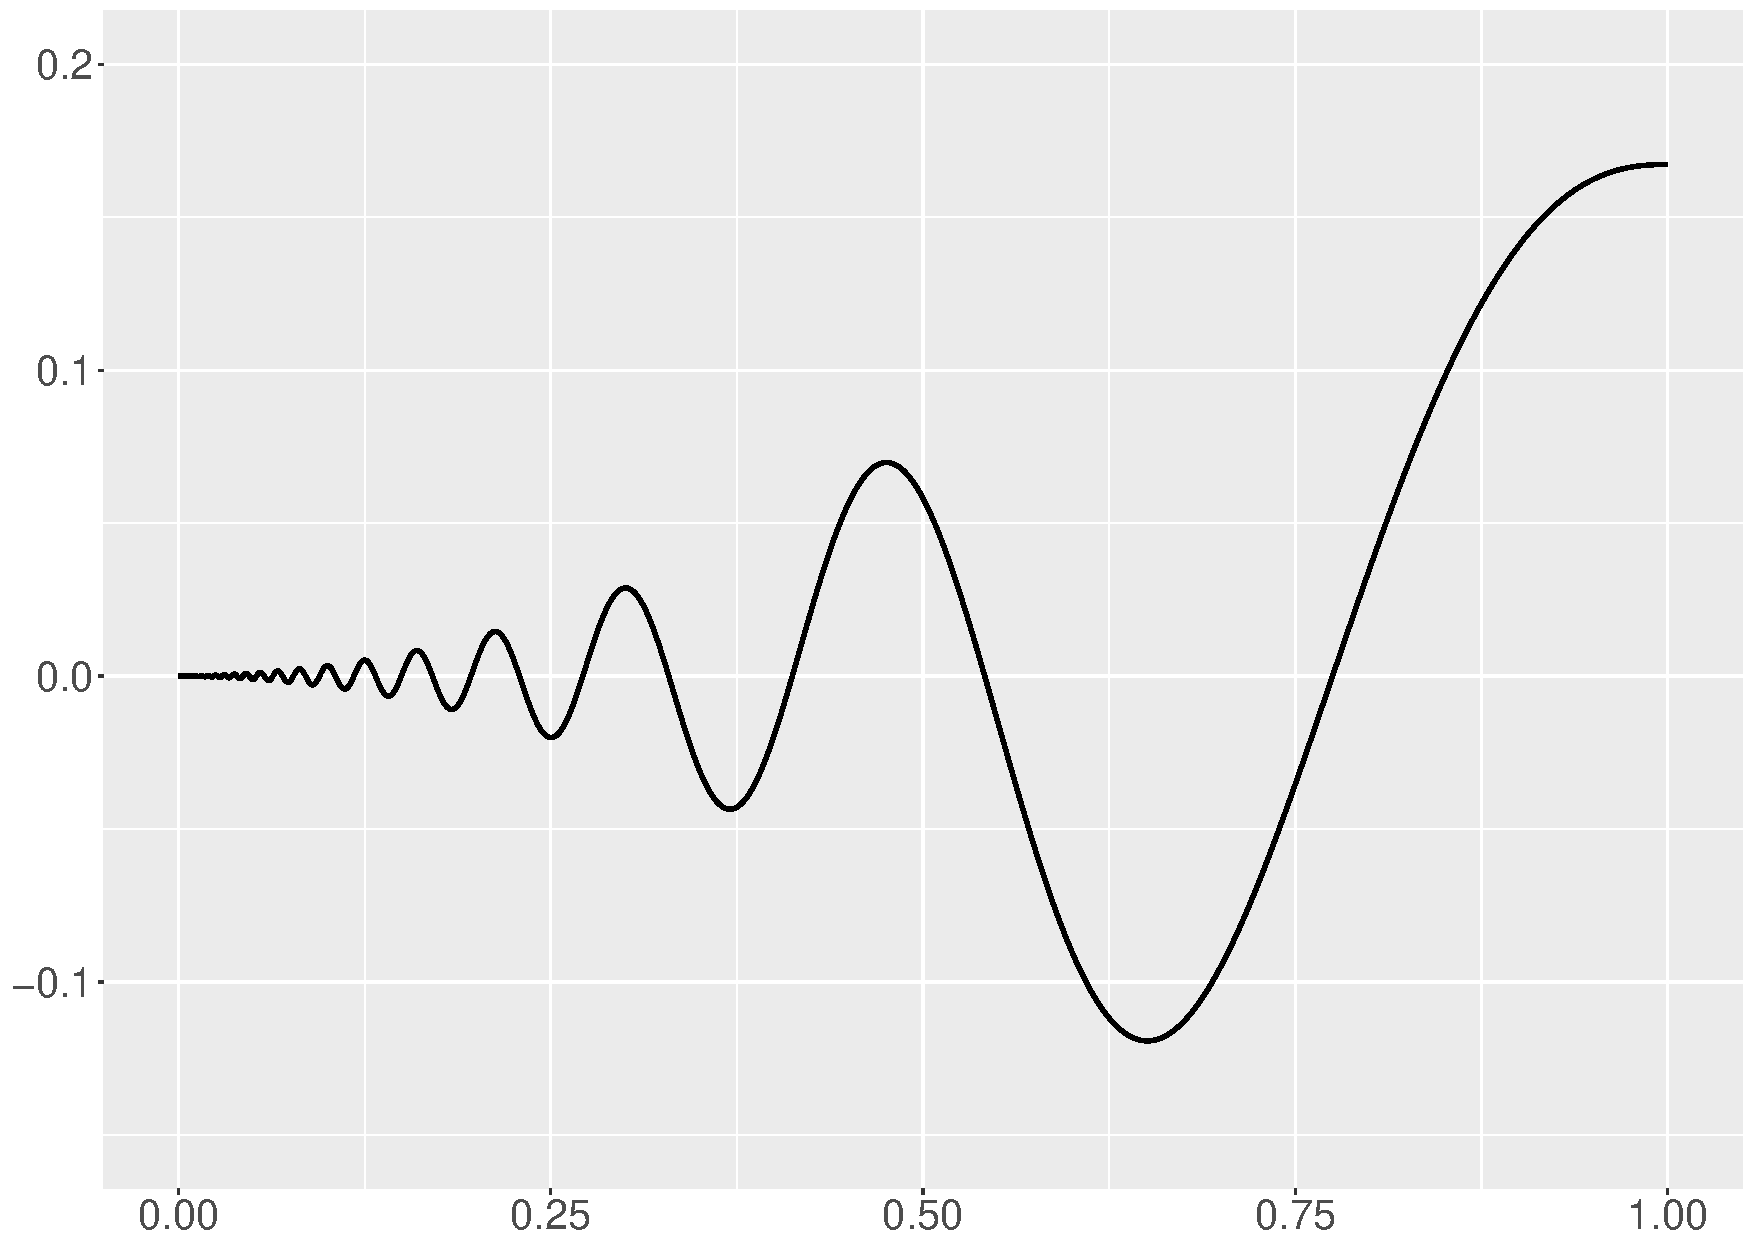
\includegraphics[width=\linewidth,height=0.45\textwidth]{Chapters/02TractorSplineTheory/plot/ggplot/ggDopplerPosition.pdf}
    \caption{Generated positions.}
    \end{subfigure}
    \begin{subfigure}{0.45\textwidth}
    \centering
    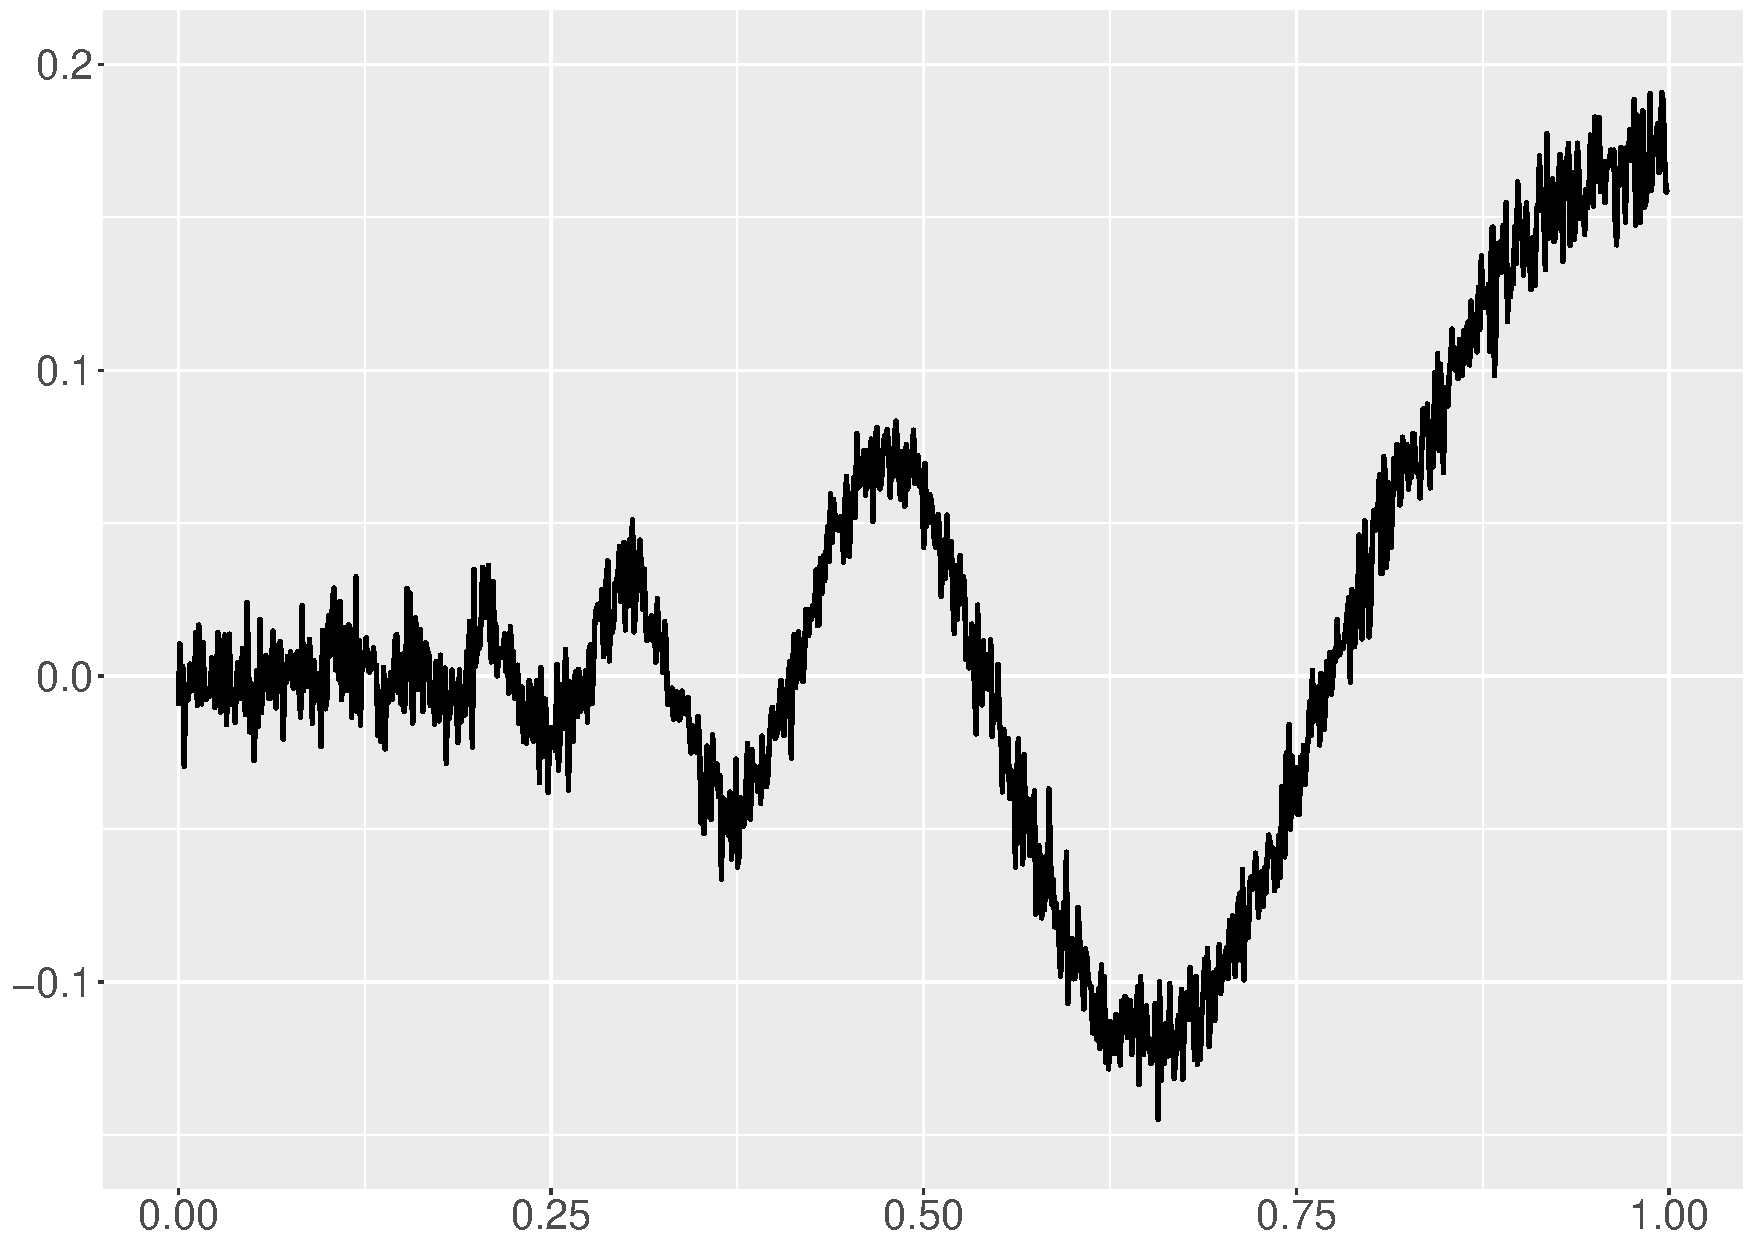
\includegraphics[width=\linewidth,height=0.45\textwidth]{Chapters/02TractorSplineTheory/plot/ggplot/ggDopplerPositionNoise.pdf}
    \caption{Noisy position at \textit{SNR}=7.}
    \end{subfigure}
    \begin{subfigure}{0.45\textwidth}
    \centering
    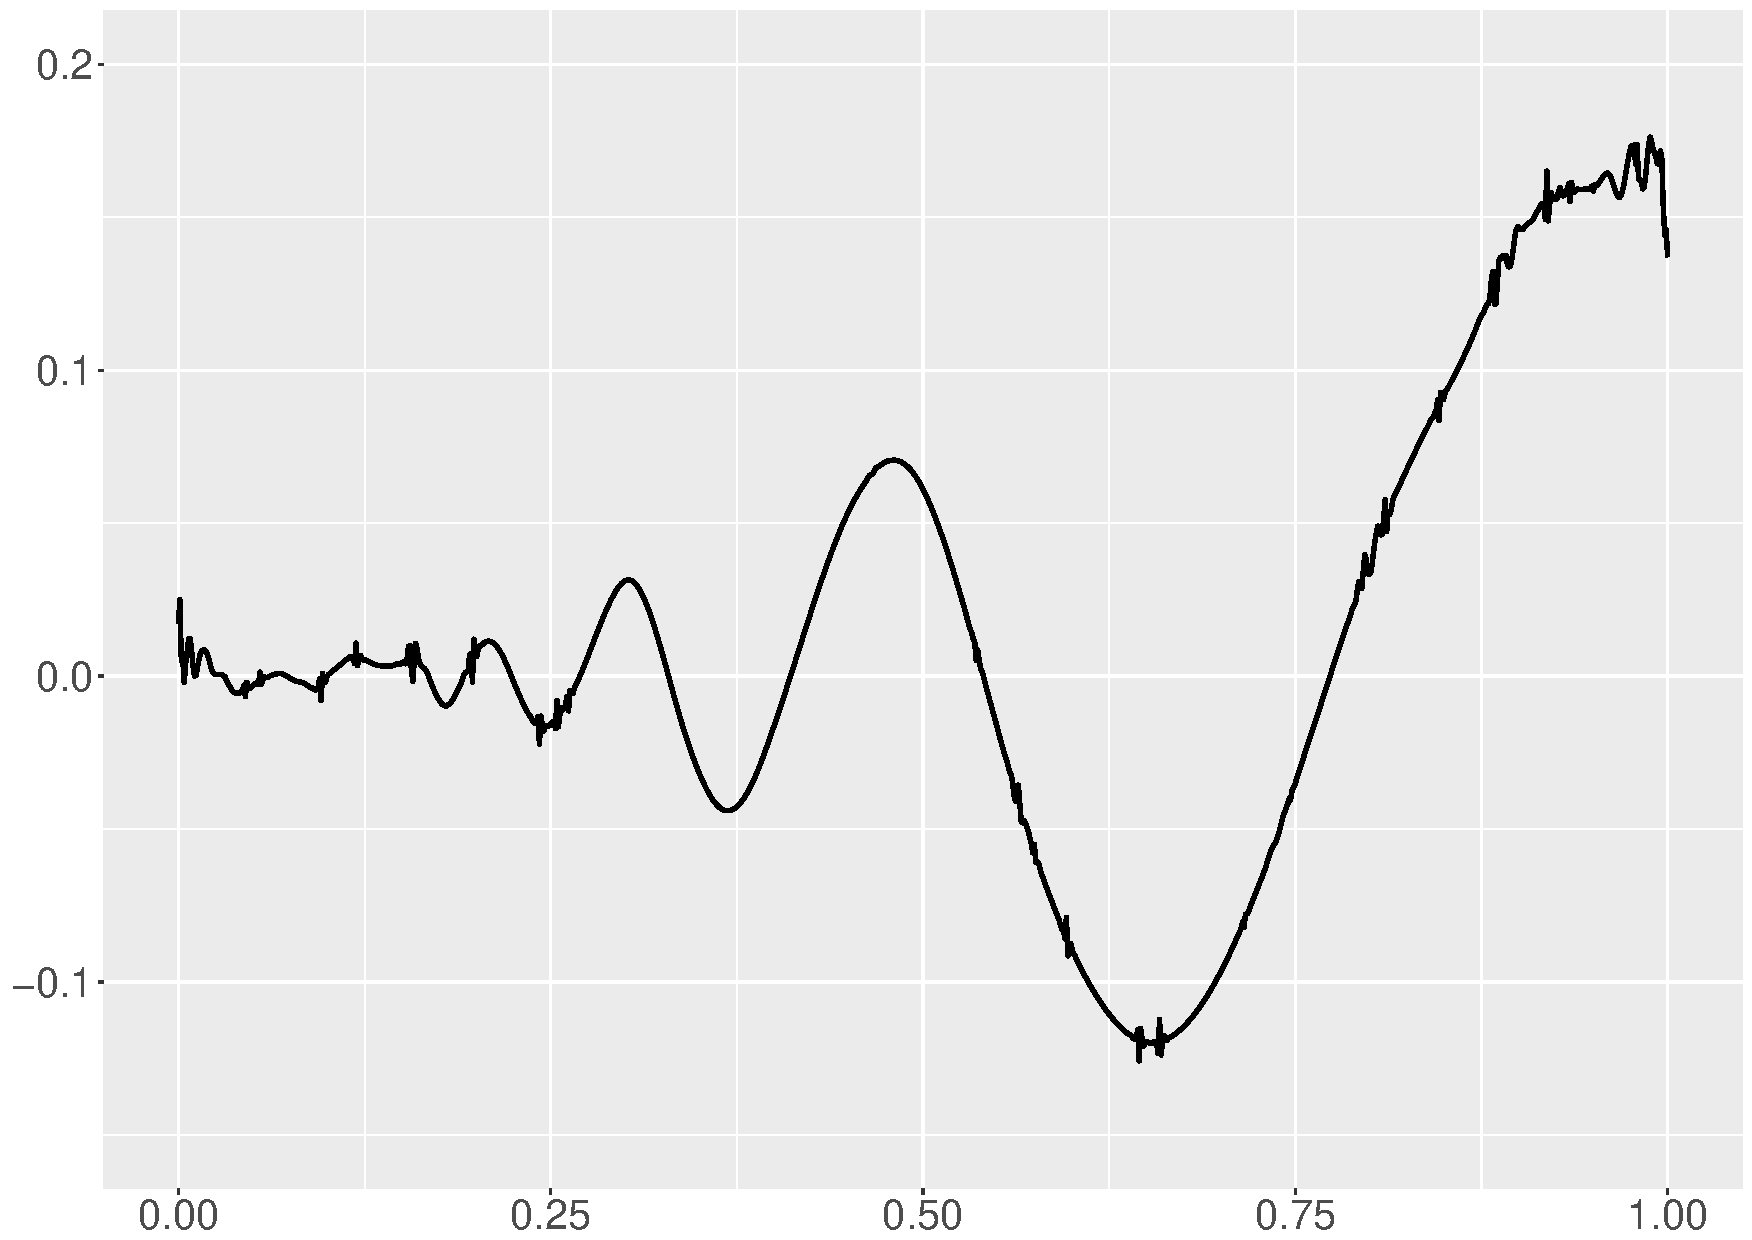
\includegraphics[width=\linewidth,height=0.45\textwidth]{Chapters/02TractorSplineTheory/plot/ggplot/ggDopplerSure.pdf}
    \caption{Reconstruction from Wavelet by sure threshold.}
    \end{subfigure}
    \begin{subfigure}{0.45\textwidth}
    \centering
    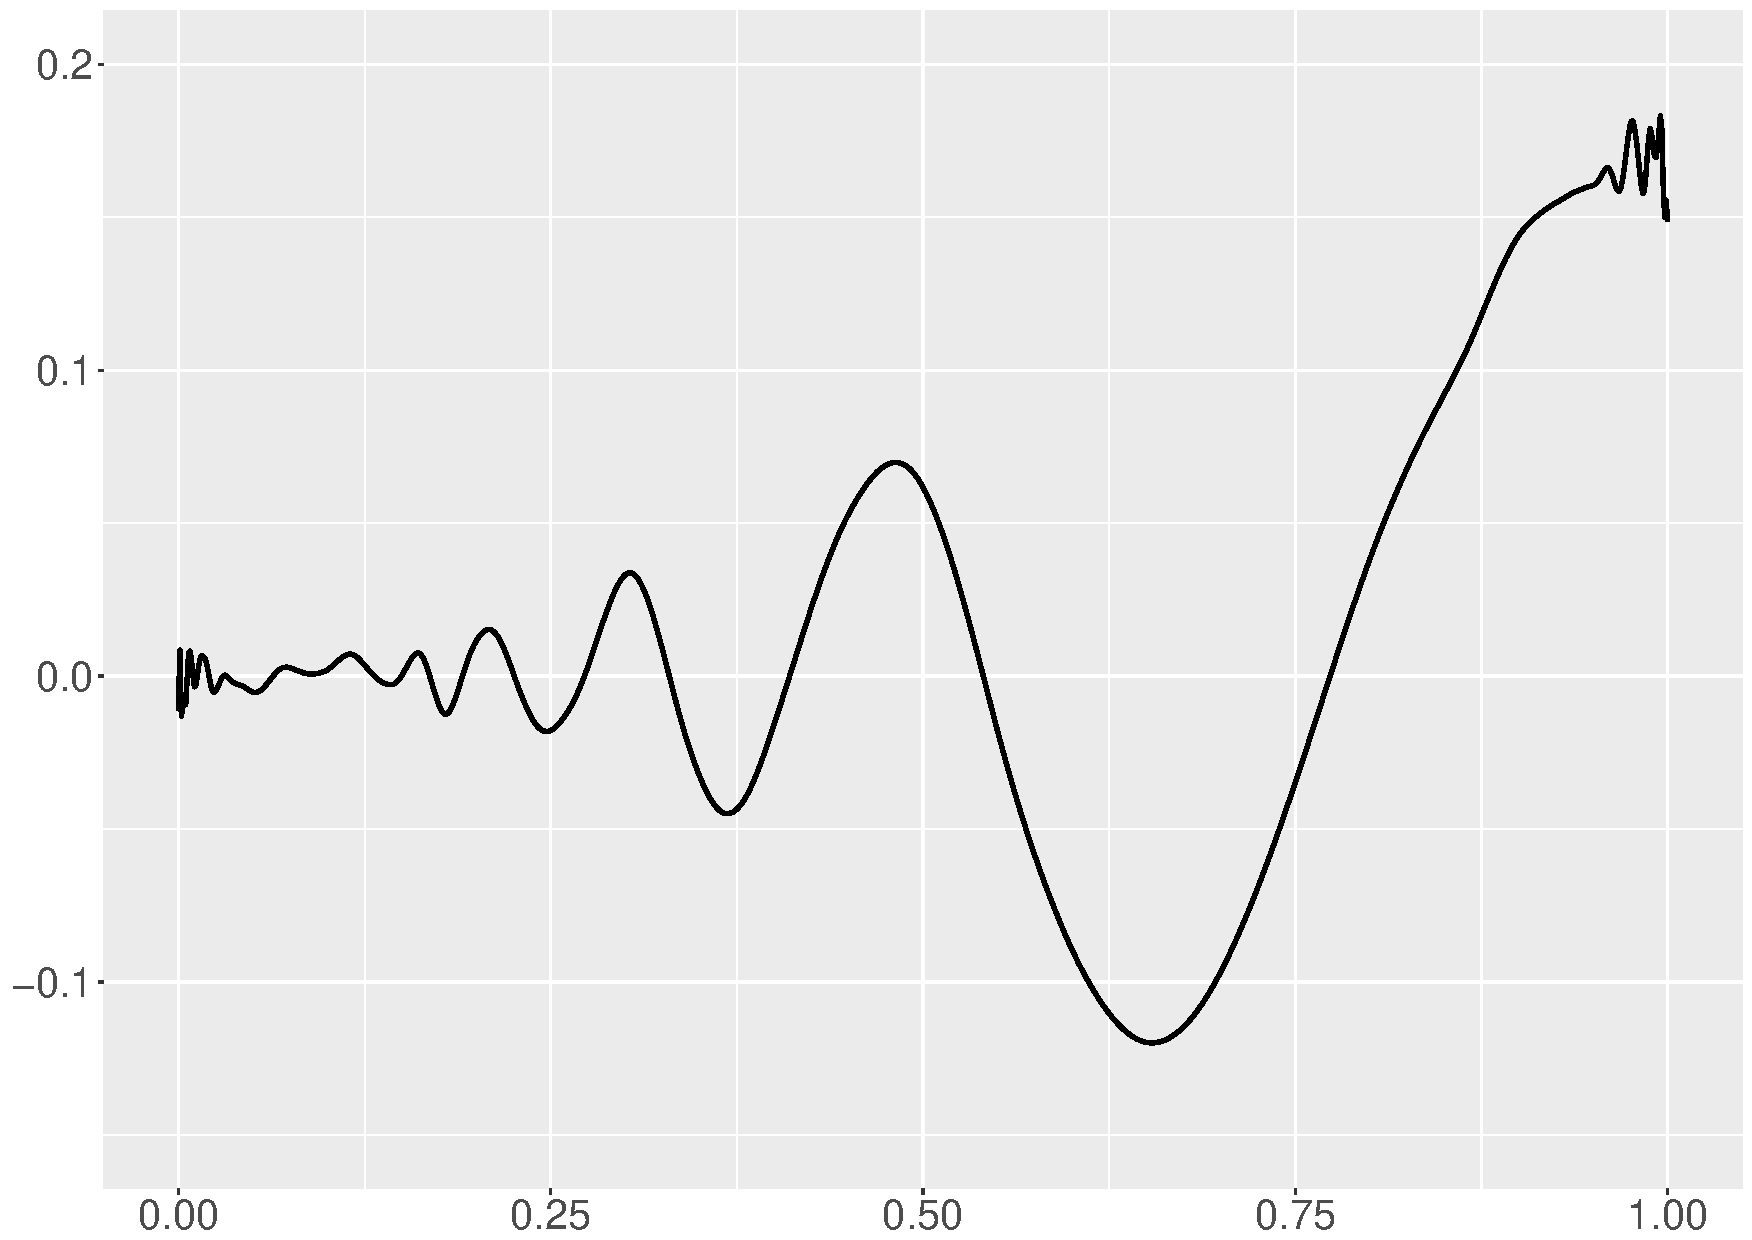
\includegraphics[width=\linewidth,height=0.45\textwidth]{Chapters/02TractorSplineTheory/plot/ggplot/ggDopplerBayes.pdf}
    \caption{Reconstruction from Wavelet by BayesThresh approach.}
    \end{subfigure}
    \begin{subfigure}{0.45\textwidth}
    \centering
    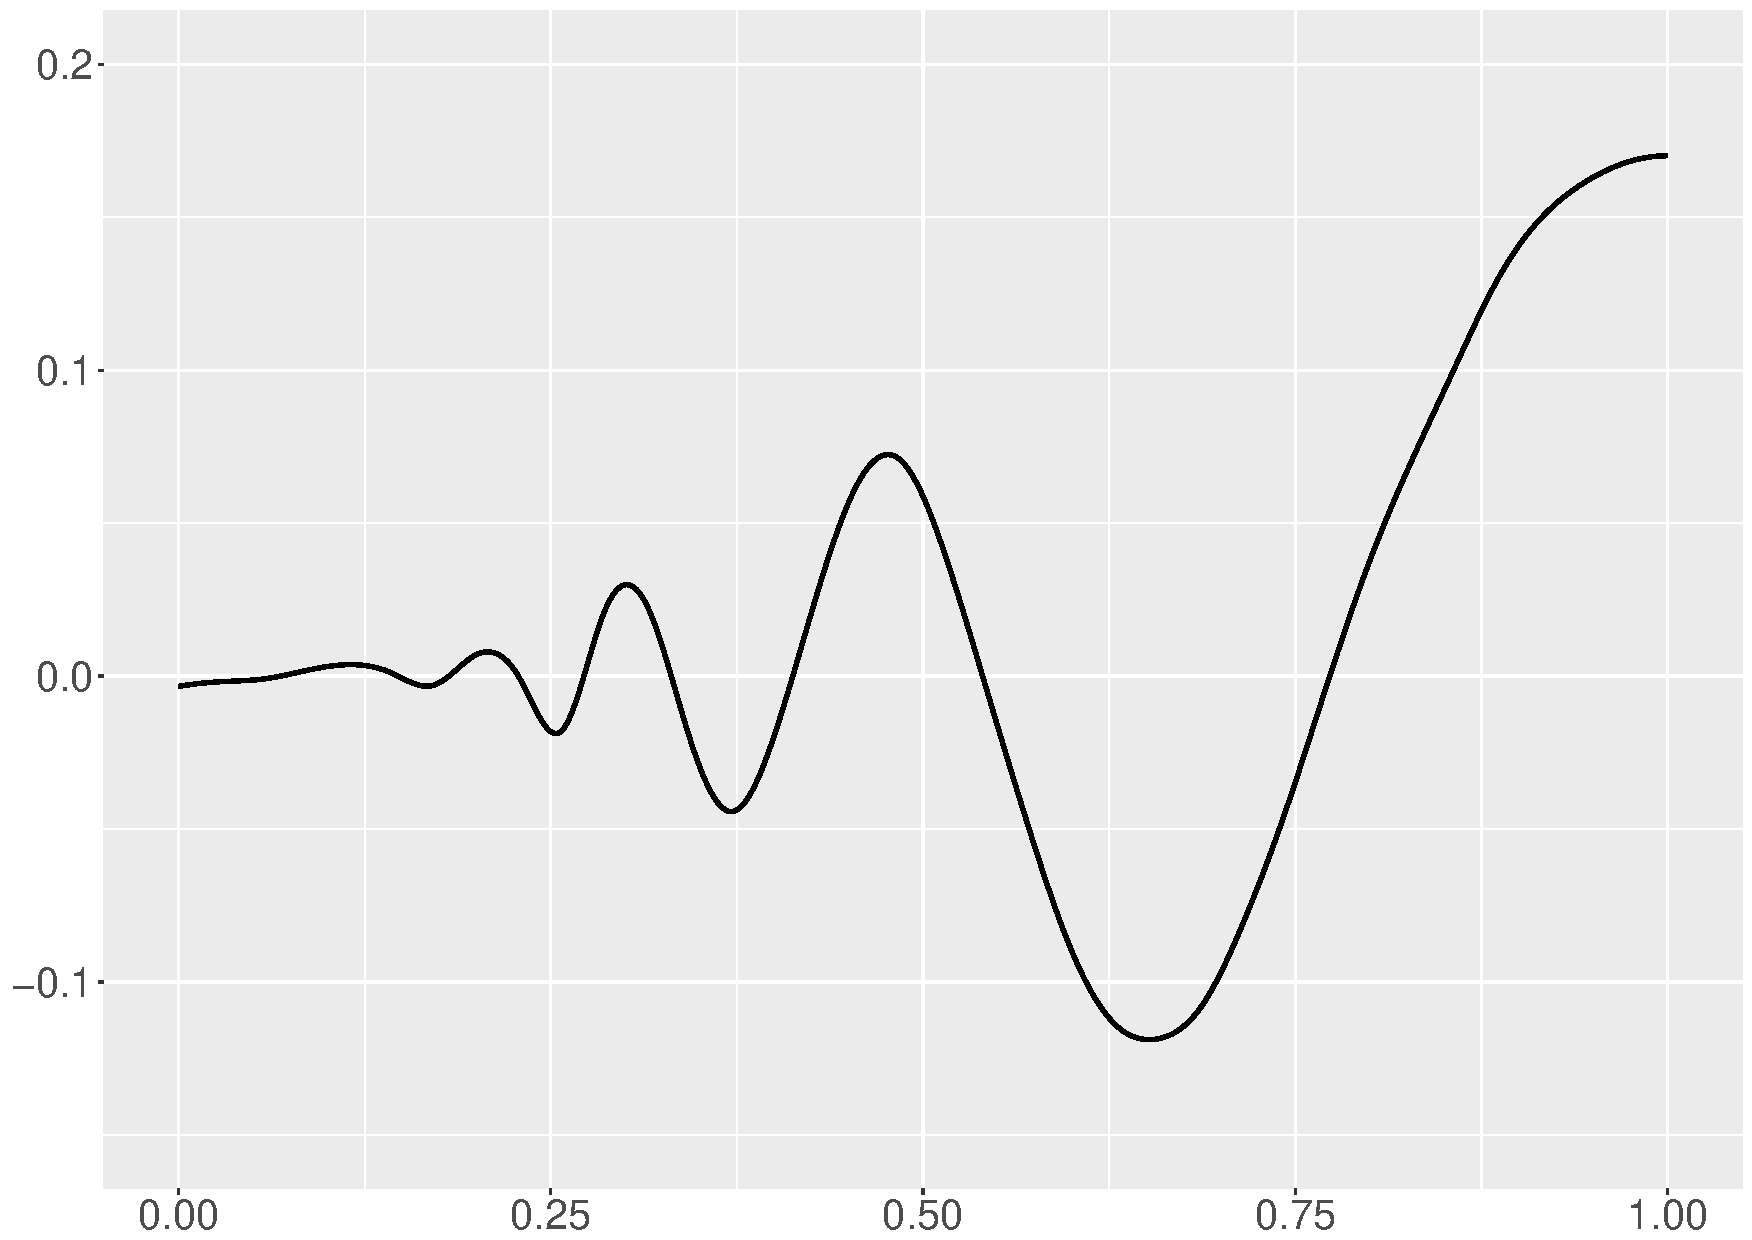
\includegraphics[width=\linewidth,height=0.45\textwidth]{Chapters/02TractorSplineTheory/plot/ggplot/ggDopplerPSpline.pdf}
    \caption{Reconstruction by P-spline. \\\mbox{  } }
    \end{subfigure}
    \begin{subfigure}{0.45\textwidth}
    \centering
    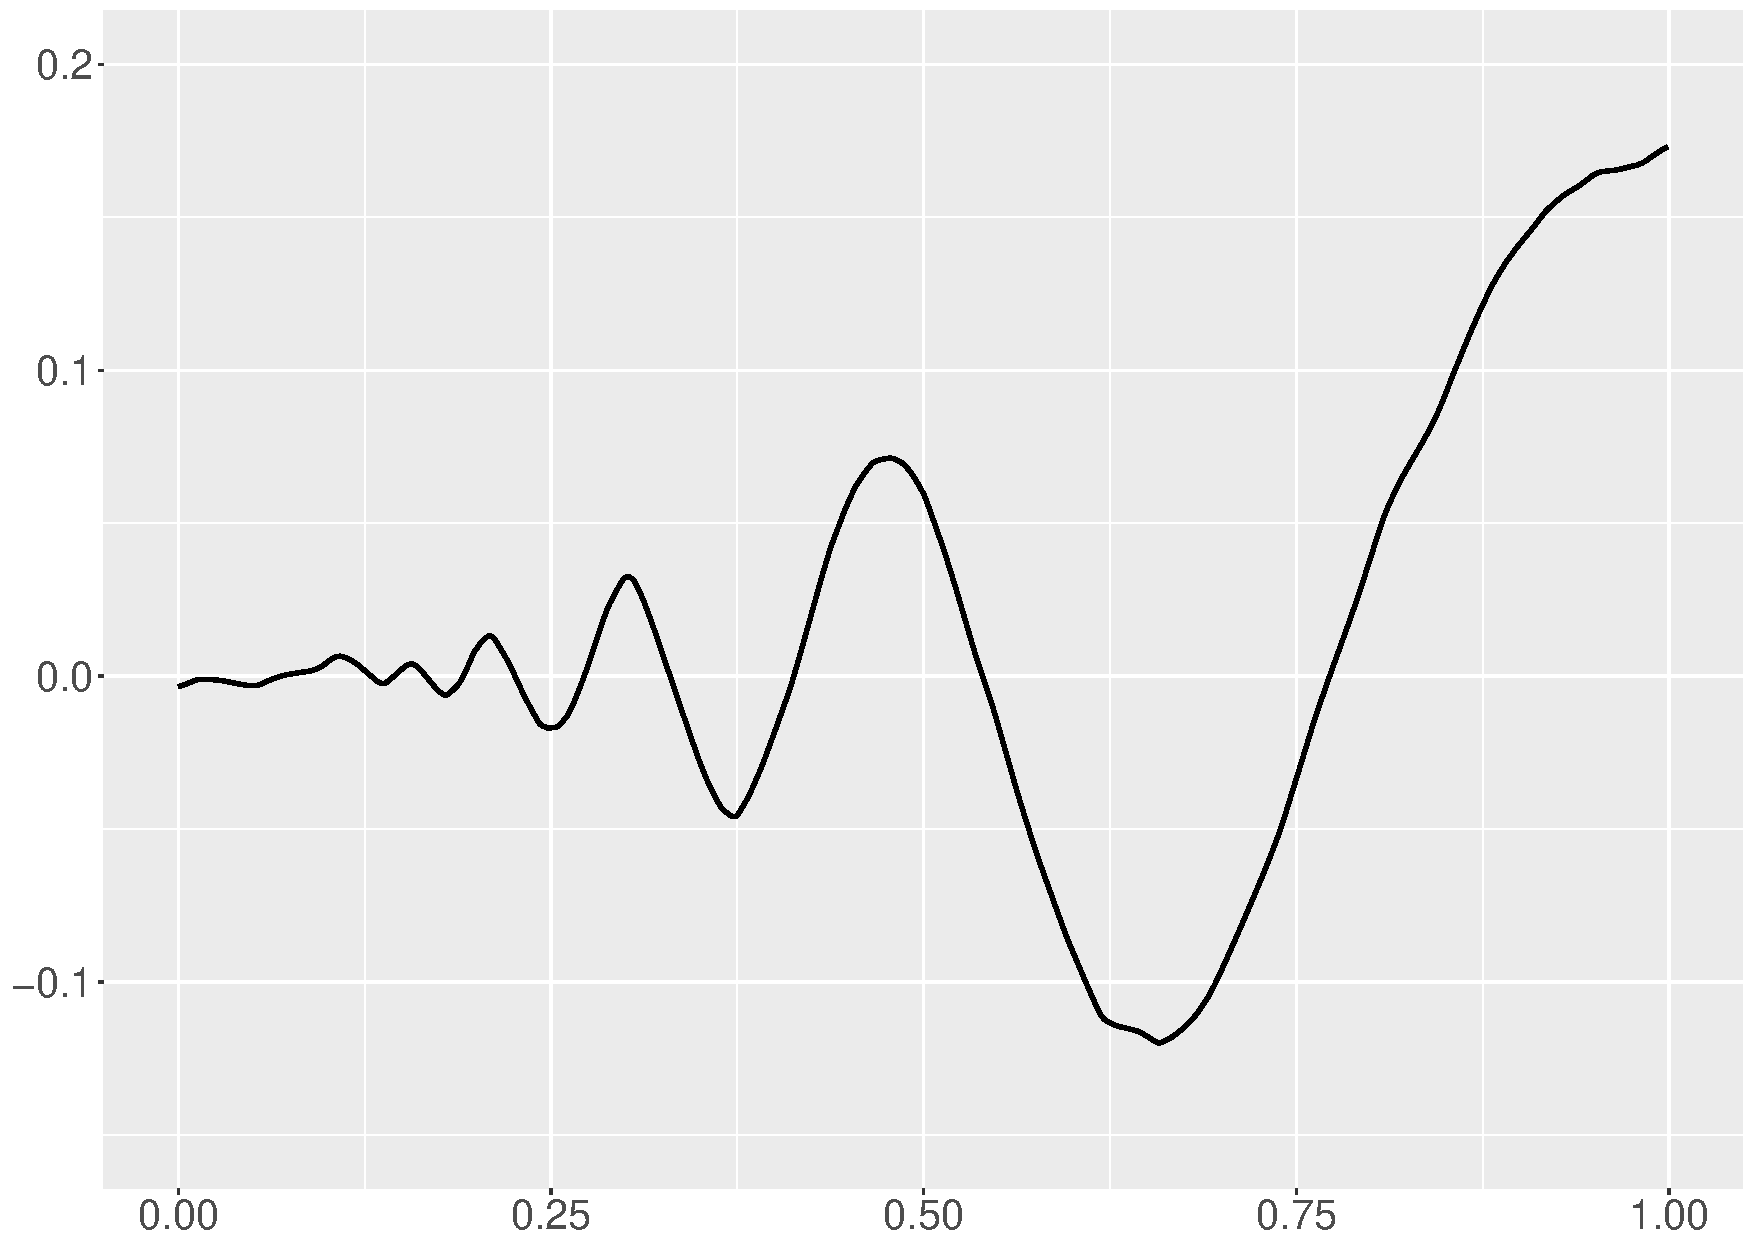
\includegraphics[width=\linewidth,height=0.45\textwidth]{Chapters/02TractorSplineTheory/plot/ggplot/ggDopplerGamma.pdf}
    \caption{Reconstruction by Tractor Spline setting $\gamma=0$}
    \end{subfigure}
  \begin{subfigure}{0.45\textwidth}
    \centering
    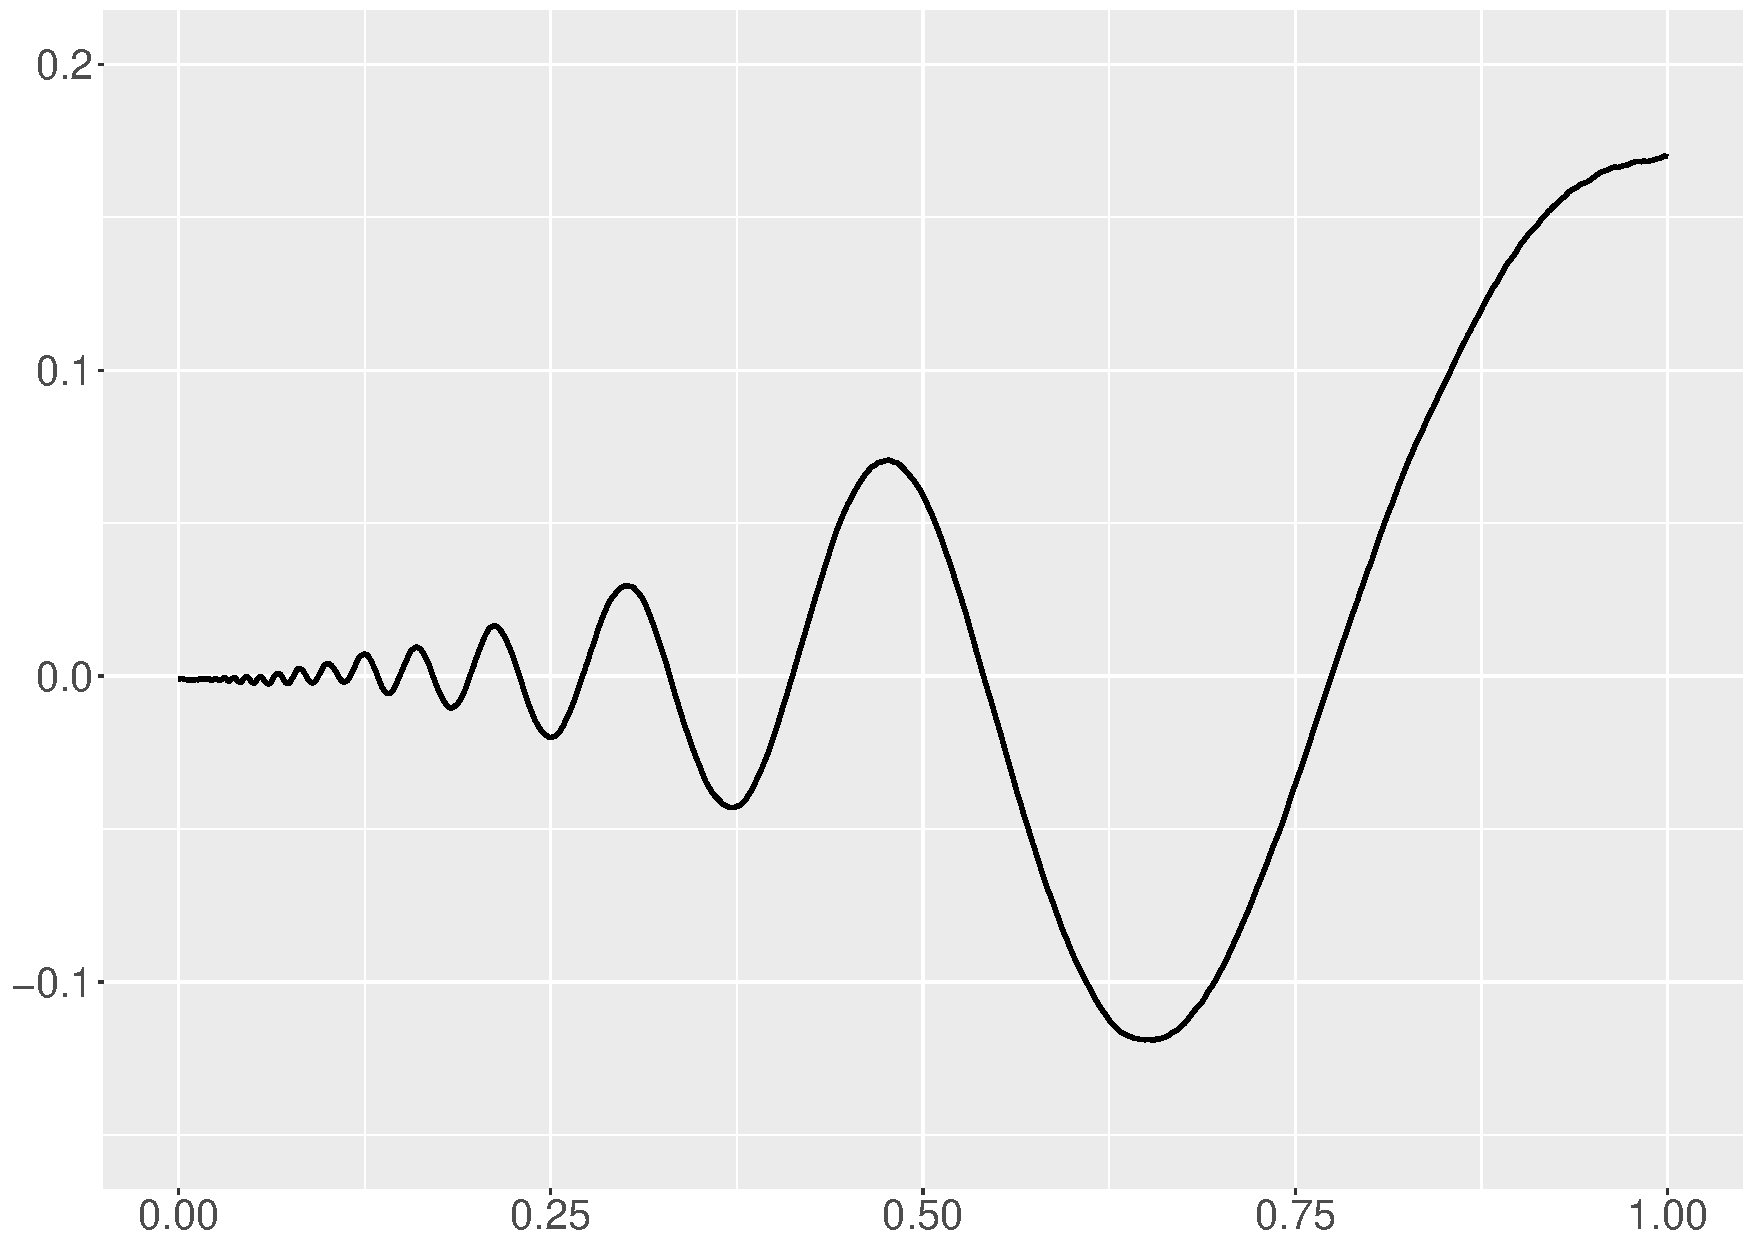
\includegraphics[width=\linewidth,height=0.45\textwidth]{Chapters/02TractorSplineTheory/plot/ggplot/ggDopplerTractorAPT.pdf}
    \caption{Reconstruction by Tractor Spline with conventional penalty term.}
    \end{subfigure}
    \begin{subfigure}{0.45\textwidth}
    \centering
    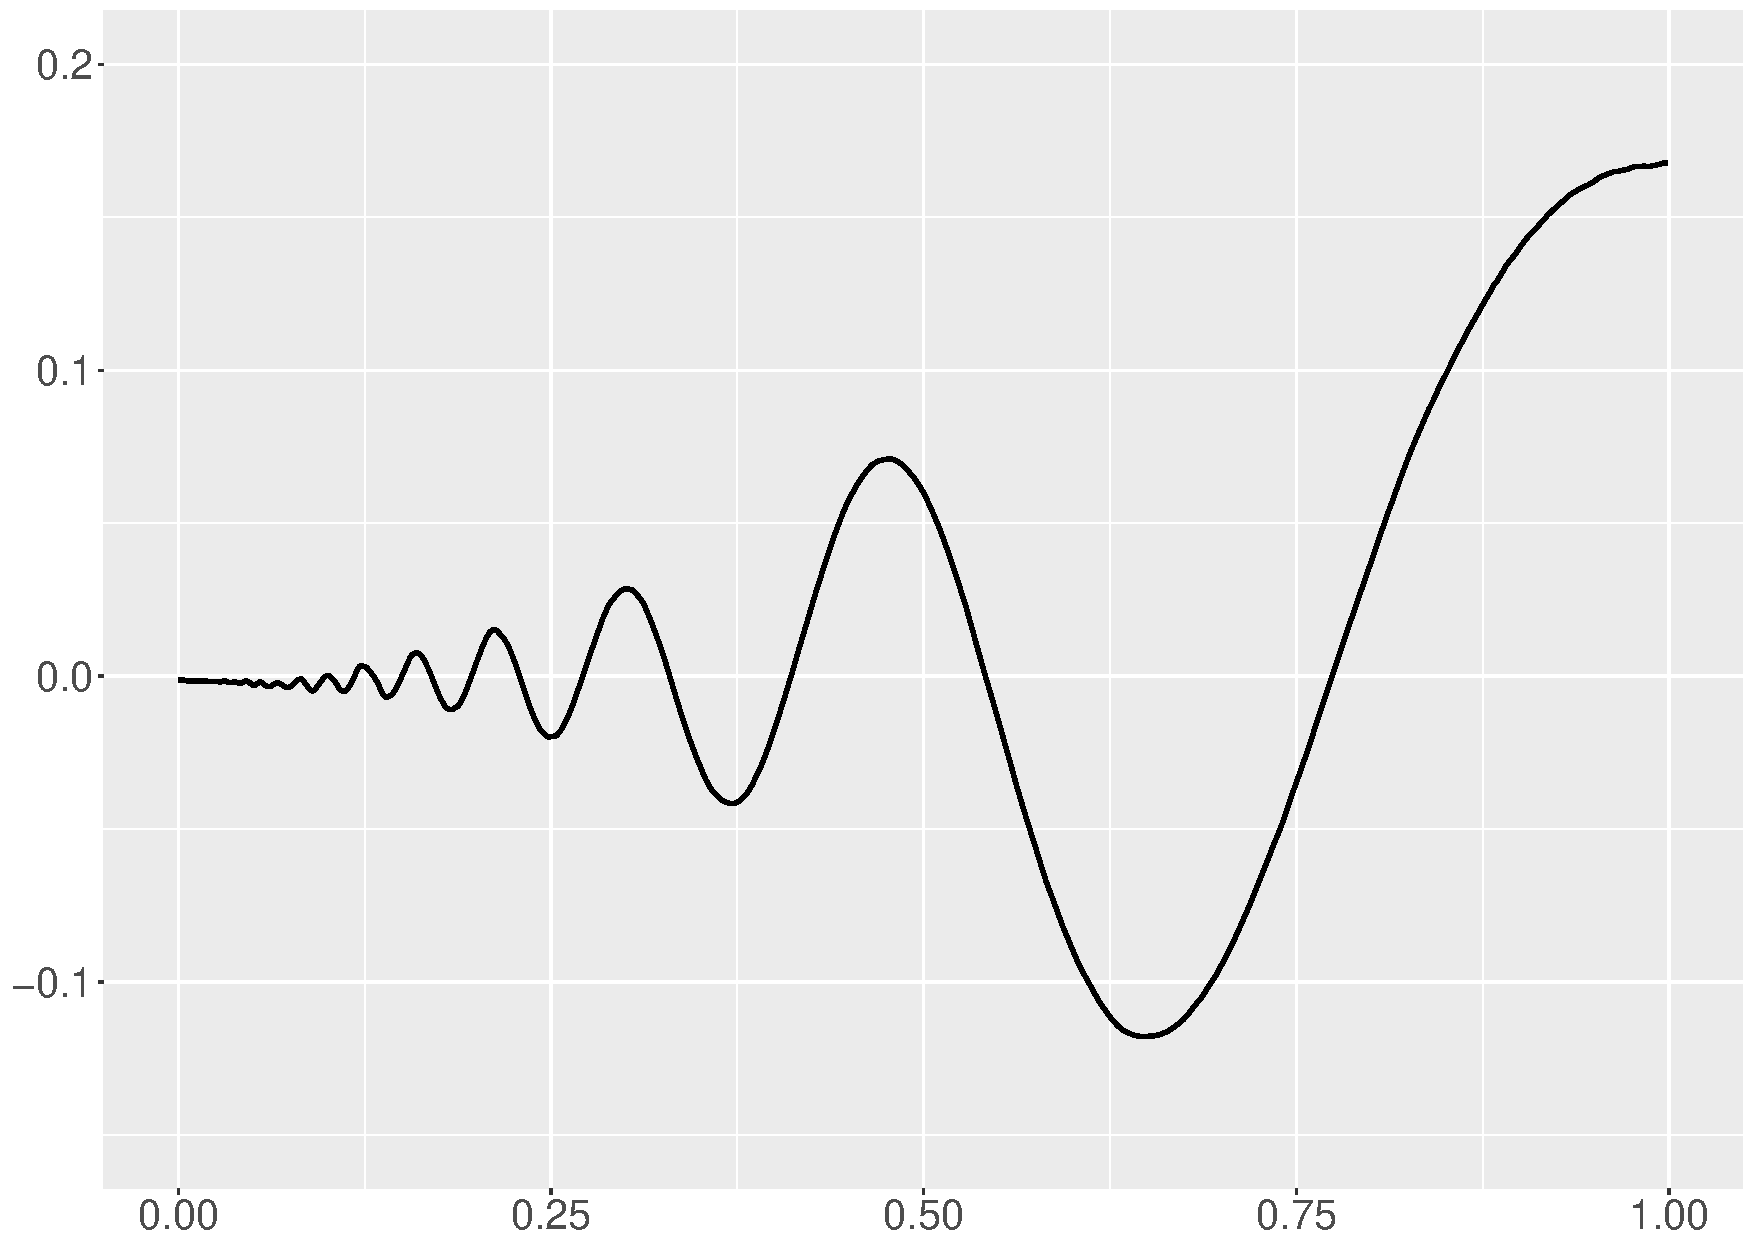
\includegraphics[width=\linewidth,height=0.45\textwidth]{Chapters/02TractorSplineTheory/plot/ggplot/ggDopplerTractor.pdf}
    \caption{Reconstruction by proposed Tractor Spline.}
    \end{subfigure}
\caption{Numerical example: $\textit{Doppler}$. Comparison of different reconstruction methods with simulated data.}\label{num4}
 \end{figure}

By comparing, we can see that all these methods can rebuild up the skeleton of generated trajectory. \textit{Wavelet(sure)} method have more wiggles in interior interval than \textit{Wavelet(BayesThresh)}, and the latter one becomes fluctuation near boundary knots. \textit{P-spline} gives much smoother fitting than wavelets, but the drawback is losing more specific details. Tractor Spline without velocity loses some information, as can be seen from \textit{Blocks} and \textit{Bumps} where there should be a straight line. Tractor Spline without adjusted penalty term get over fitting when the direction changes more frequently than normal, although it catches specific feature in \textit{HeaviSine}. The proposed Tractor Spline performs much better than other methods and returns the near-true trajectory reconstructions.  



%and is larger when the function trying to change directions. We only have a couple of large penalty terms in $\textit{Blocks}$ and $\textit{Bumps}$ function, as most of the time they were moving in straight line. More curves are in $\textit{HeaviSine}$ and $\textit{Doppler}$ functions, so the penalty term try to catch more information and ignore noises. 
%\begin{figure}
%  \centering
%         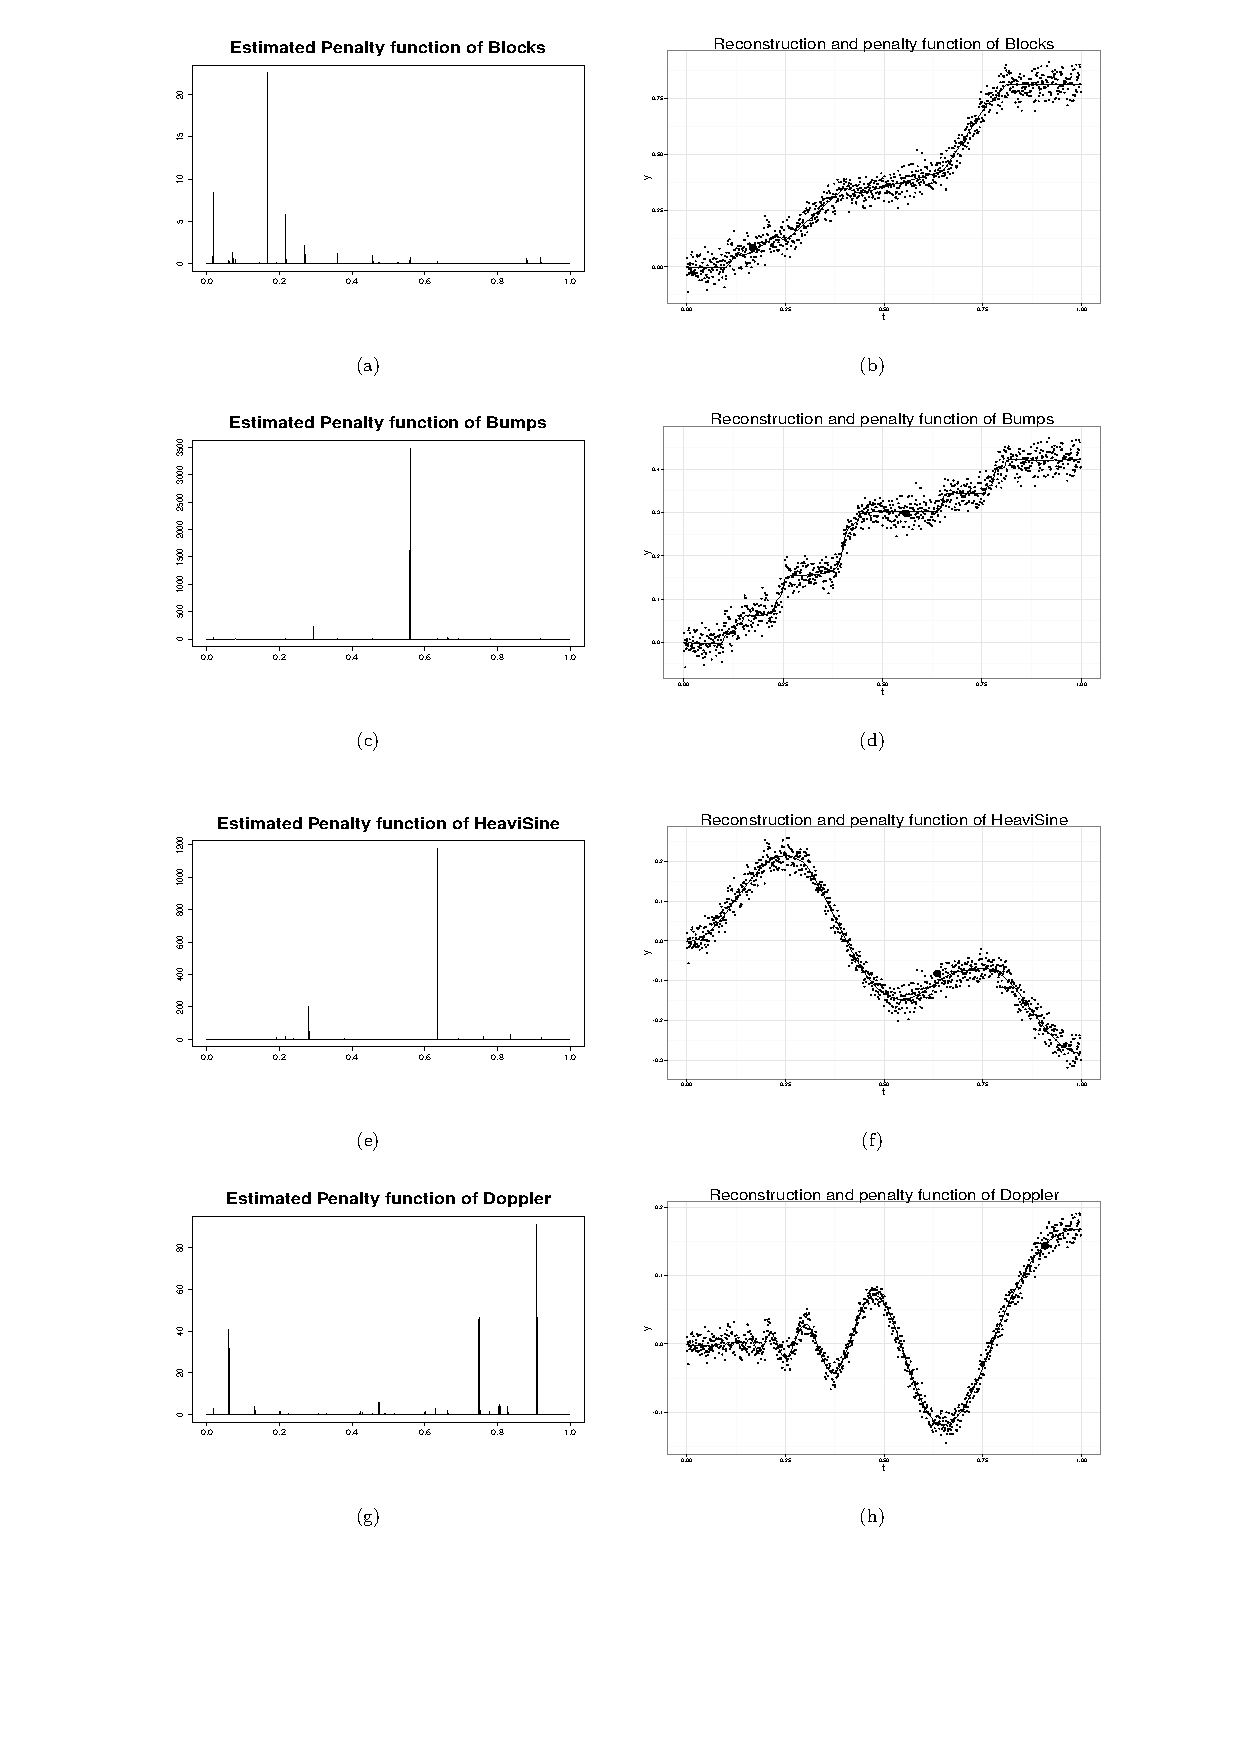
\includegraphics[width=\textwidth,height=14cm]{Chapters/02TractorSplineTheory/plot/penalty08} 
%  \caption{Estimated penalty functions. Left side shows how the value of $\lambda(t)$ changes on the interval. Right side projects $\lambda(t)$ into reconstructions. The bigger the blacks dots present, the larger the penalty values are.}\label{numpenalty}
%\end{figure}



\begin{figure}
    \centering
    \begin{subfigure}{\textwidth}
    \centering
    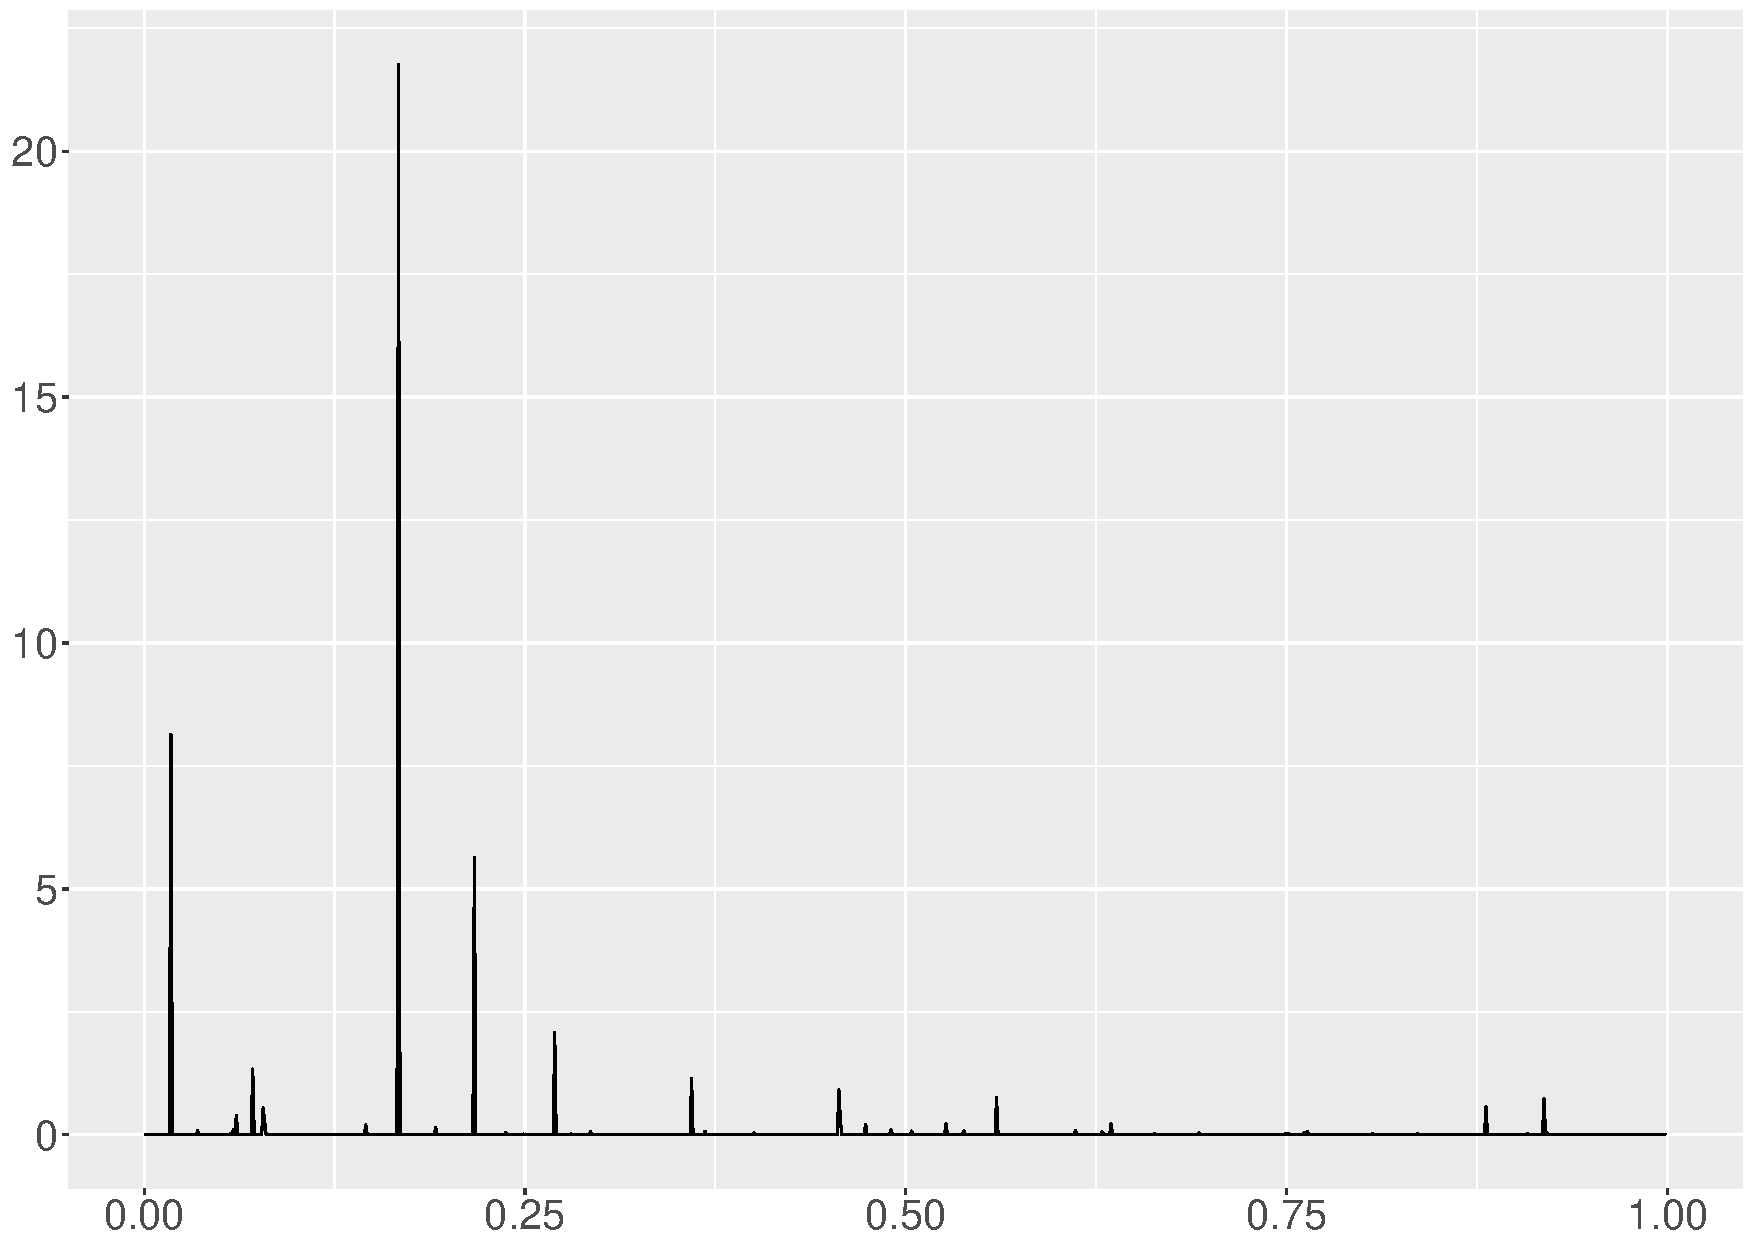
\includegraphics[width=0.45\linewidth]{Chapters/02TractorSplineTheory/plot/ggplot/ggBlocksPenaltyBar.pdf}
    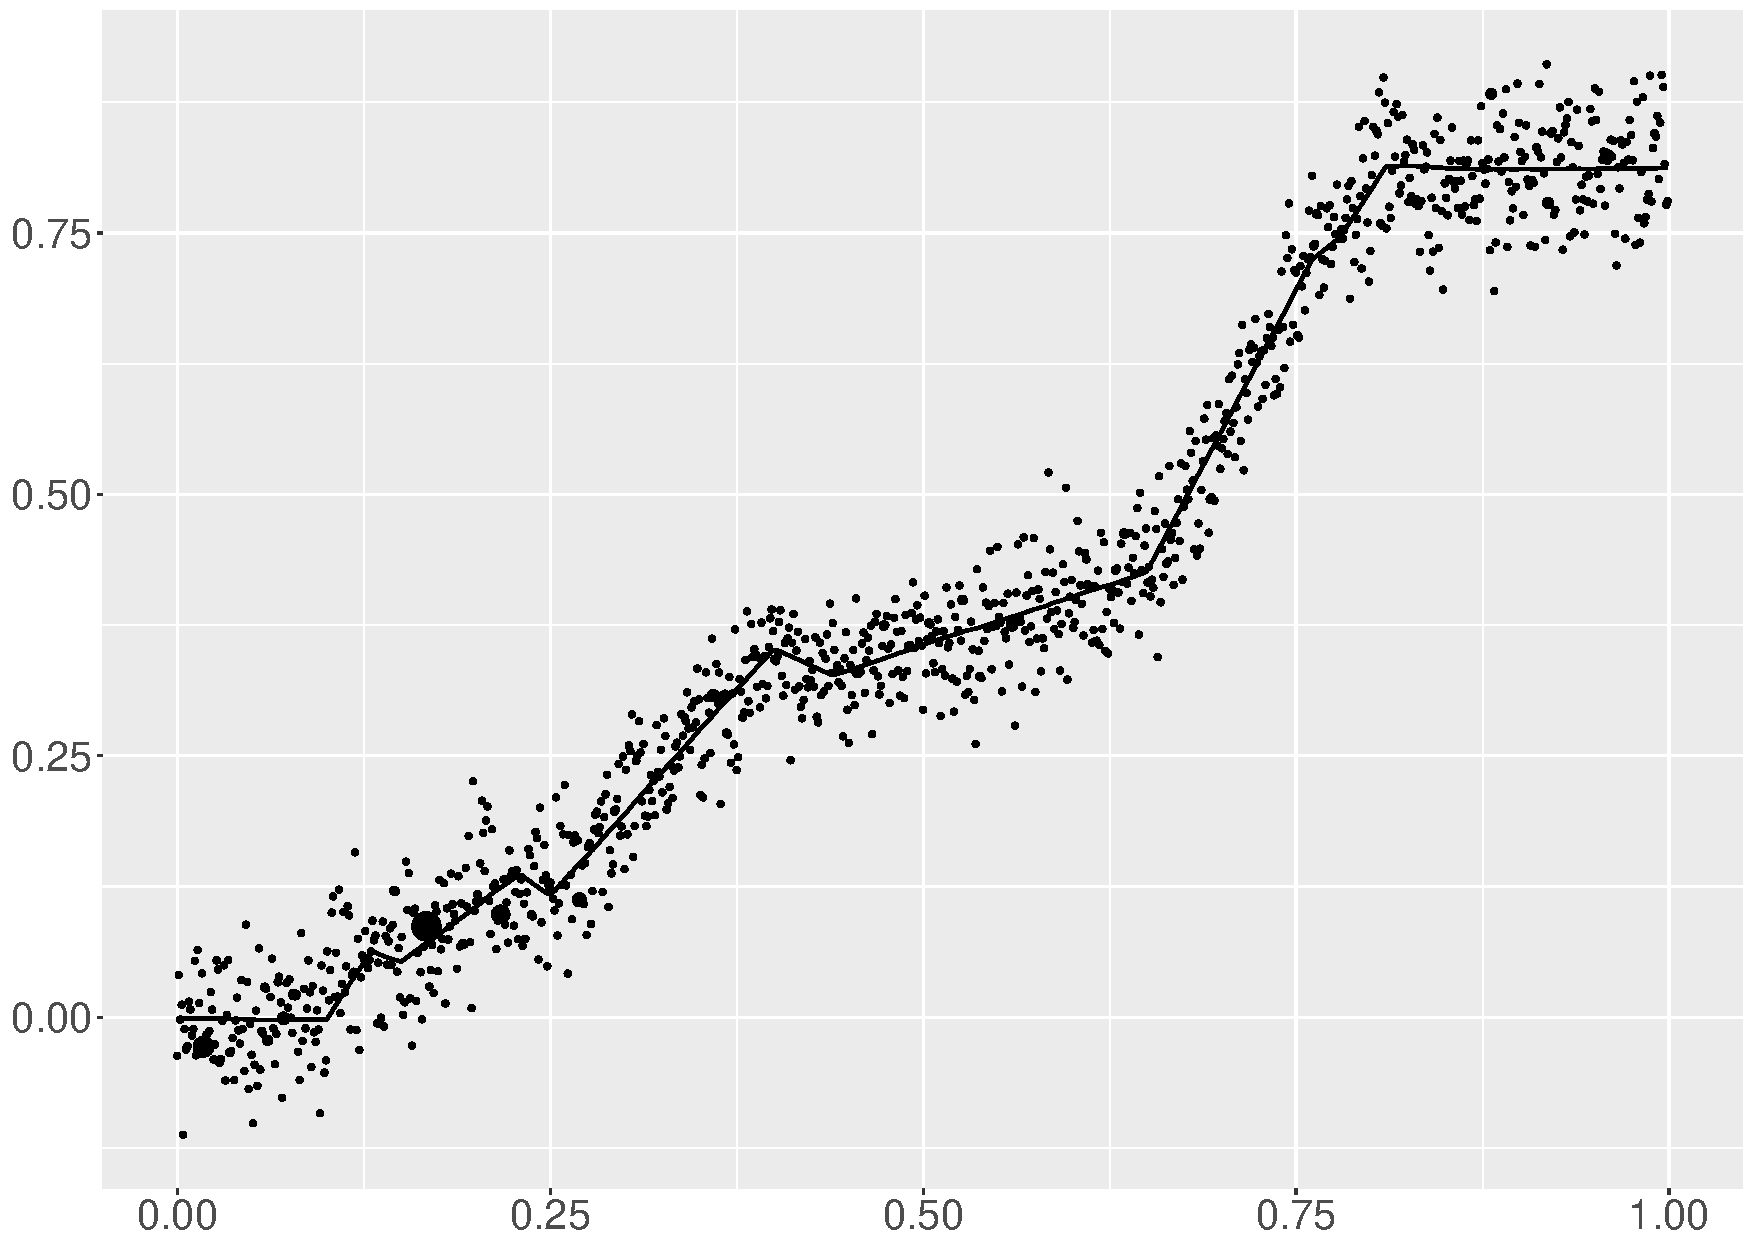
\includegraphics[width=0.45\linewidth]{Chapters/02TractorSplineTheory/plot/ggplot/ggBlocksPenaltyLine.pdf}
    \caption{Distribution of penalty values in reconstructed \textit{Blocks} function.}
    \end{subfigure}
    \begin{subfigure}{\textwidth}
    \centering
    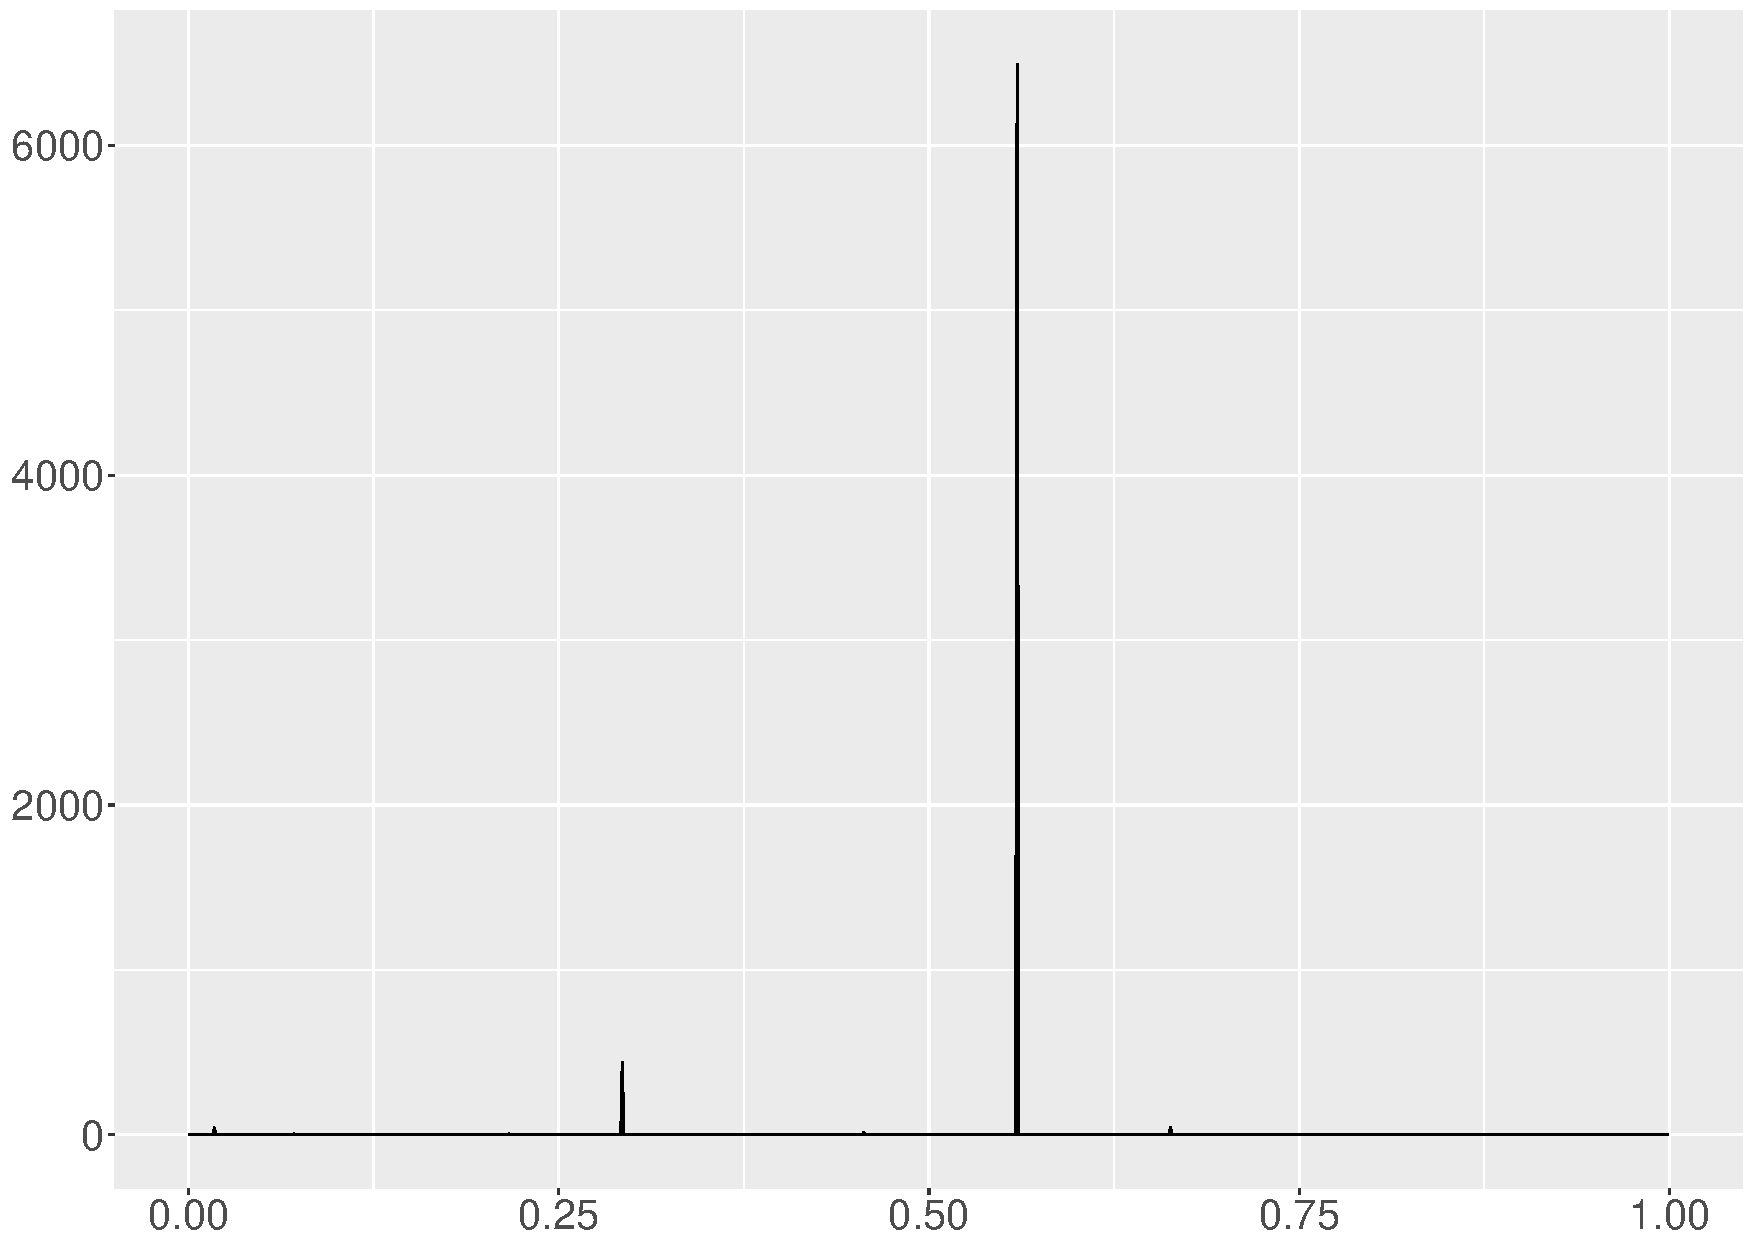
\includegraphics[width=0.45\linewidth]{Chapters/02TractorSplineTheory/plot/ggplot/ggBumpsPenaltyBar.pdf}
    \includegraphics[width=0.45\linewidth]{Chapters/02TractorSplineTheory/plot/ggplot/ggBumpsPenaltyLine.pdf}
    \caption{Distribution of penalty values in reconstructed \textit{Bumps} function.}
    \end{subfigure}
    \begin{subfigure}{\textwidth}
    \centering
    \includegraphics[width=0.45\linewidth]{Chapters/02TractorSplineTheory/plot/ggplot/ggHeaviSinePenaltyBar.pdf}
    \includegraphics[width=0.45\linewidth]{Chapters/02TractorSplineTheory/plot/ggplot/ggHeaviSinePenaltyLine.pdf}
    \caption{Distribution of penalty values in reconstructed \textit{HeaviSine} function.}
    \end{subfigure}
    \begin{subfigure}{\textwidth}
    \centering
    \includegraphics[width=0.45\linewidth]{Chapters/02TractorSplineTheory/plot/ggplot/ggDopplerPenaltyBar.pdf}
    \includegraphics[width=0.45\linewidth]{Chapters/02TractorSplineTheory/plot/ggplot/ggDopplerPenaltyLine.pdf}
    \caption{Distribution of penalty values in reconstructed \textit{Doppler} function.}
    \end{subfigure}
\caption{Distribution of penalty values in reconstructed Tractor Spline. Figures on left side indicate the values of $\lambda(t)$ varying in intervals. On right side, $\lambda(t)$ is projected into reconstructions. The bigger the blacks dots present, the larger the penalty values are.}\label{numpenalty}
 \end{figure}



Figure \ref{numpenalty} shows the estimated penalty function
\begin{equation}
\lambda(t)=\frac{(\Delta t)^3}{(\Delta d)^2}\lambda.
\end{equation}
The left column illustrates the value of penalty function on different intervals and the right column is the projection on position. Bigger black dots present larger penalty values. It can be seen that $\lambda(t)$ adapts to the smoothness pattern of position and will be large where a long time gap may occur. The details of how this penalty function works will be explained in next subsection.


%\begin{figure}
%\centering
%%  \begin{landscape}
%         \includegraphics[width=\textwidth,height=9cm]{Chapters/02TractorSplineTheory/plot/vtractor04} 
%%  \end{landscape}
%     \caption{Estimated velocity functions by taking the first derivative of Tractor Spline. (a) Fitted $\textit{Blocks}$. (b) Fitted $\textit{Bumps}$. (c) Fitted $\textit{HeaviSine}$. (d) Fitted $\textit{Doppler}$.}\label{numvtractor}
%\end{figure}

\begin{figure}
    \centering
    \begin{subfigure}{0.45\textwidth}
    \centering
    \includegraphics[width=\linewidth,height=0.45\textwidth]{Chapters/02TractorSplineTheory/plot/ggplot/ggBlocksTractorVelocity.pdf}
    \caption{Estimated \textit{Blocks}  }
    \end{subfigure}%
    \begin{subfigure}{0.45\textwidth}
    \centering
    \includegraphics[width=\linewidth,,height=0.45\textwidth]{Chapters/02TractorSplineTheory/plot/ggplot/ggBumpsTractorVelocity.pdf}
    \caption{Estimated \textit{Bumps}  }
    \end{subfigure}
    \begin{subfigure}{0.45\textwidth}
    \centering
    \includegraphics[width=\linewidth,height=0.45\textwidth]{Chapters/02TractorSplineTheory/plot/ggplot/ggHeaviSineTractorVelocity.pdf}
    \caption{Estimated \textit{HeaviSine}  }
    \end{subfigure}
    \begin{subfigure}{0.45\textwidth}
    \centering
    \includegraphics[width=\linewidth,height=0.45\textwidth]{Chapters/02TractorSplineTheory/plot/ggplot/ggDopplerTractorVelocity.pdf}
    \caption{Estimated \textit{Doppler}  }
    \end{subfigure}
\caption{Estimated velocity functions (original simulation functions) by Tractor Spline.}\label{numvtractor}
 \end{figure}



Figure \ref{numvtractor} demonstrates the estimated velocity functions. By taking the first derivative of fitted tractor spine, it is easily to get the original four velocity functions. The fitting of velocity is not as smooth as that in position, because we only care about the smoothness of position rather than velocity in our cross-validation formula (\ref{cvscore}). However, velocity information do help us reconstruct the trajectory.



\subsection{Evaluation}
To examine the performance of Tractor Spline, we conducted a evaluation by comparing the mean square errors and true mean square errors, which are respectively calculated in
\begin{align}
\mbox{MSE}&= \frac{1}{n} \sum_{i=1}^{n} (y_i-\hat{f}_{\lambda,\gamma}(t_i))^2,\\
\mbox{TMSE}&= \frac{1}{n} \sum_{i=1}^{n} (f(t_i)-\hat{f}_{\lambda,\gamma}(t_i))^2.
\end{align}


%Besides the four function in previous subsection, we introduce two more functions as the author did in \cite{liu2010data}: Sin-141 and Sin-1414. The function Sin-141 is divided into three equal length intervals $B_1\oplus B_2 \oplus B_3$ on $[0,1]$ with signal generated by $sin(6\pi t)I\{t\in (B_1,B_3)\} + sin(24\pi t)I(t\in B_2)$, where $I(\cdot)$ is the indicator function. Sin-1414 is divided into four equal length intervals $B_1\oplus B_2 \oplus B_3 \oplus B_4$ on $[0,1]$ with signal generated by $sin(6\pi t)I\{t\in (B_1,B_3)\} + sin(24\pi t)I(t\in B_2,B_4)$

The results are shown in table \ref{mse3200} and \ref{tmse3200}. All of these methods have good performances in fitting noisy data. The differences of mean square error between these methods are not significant, as can be seen from table \ref{mse3200}. The proposed method is not the best among these simulations according to MSE. However, from table \ref{tmse3200}, Tractor Spline returns the smallest true mean square errors. The difference is significant, that means the reconstruction from Tractor Spline is closer to the true trajectory. 
 
%\begin{sidewaystable}
 \begin{table}
 	\centering
 	\caption{MSE. Mean square errors of different methods. The numbers in bold indicate the smallest error among these methods under the same level. The difference is not significant.}\label{mse3200}
	\setlength\tabcolsep{1.5pt}
	\begin{tabular}{|c|c|c|c|c|c|c|c|}
\hline	MSE ($10^{-4}$)   & SNR & TS & TS$_{\gamma=0}$ & TS$_{APT=0}$  & P-spline & Wavelet(sure)& Wavelet(Bayes)\\ \hline
\textit{Blocks}    & 7   &  16.53& 15.99 & 16.69 & 16.14  & \textbf{15.39} & 16.68 \\ \hline
\textit{Blocks}    & 3   &  89.79 & \textbf{87.64} & 89.94  & 88.27 & 98.35 & 90.24 \\ \hline
\textit{Bumps}     & 7   & 4.40 & 4.19 & 4.55 & 4.33 & \textbf{4.18} & 4.59 \\ \hline
\textit{Bumps}     & 3   & 23.93 & \textbf{23.19} & 24.10 & 23.55 & 26.23 & 23.74 \\ \hline
\textit{HeaviSine} & 7   & 4.16 & 4.01 &4.16 & 4.02 & \textbf{3.79} & 4.19 \\ \hline
\textit{HeaviSine} & 3   & 22.63 & \textbf{22.19} & 22.65 & 22.02 & 23.53 & 22.07 \\ \hline
\textit{Doppler}   & 7   & 1.15 & \textbf{1.07} & 1.10 & 1.15  & \textbf{1.07} & 1.13  \\ \hline
\textit{Doppler}   & 3   & 6.27 & \textbf{5.94} &6.28 & 6.05  & 6.85 & 6.29  \\ \hline
	\end{tabular}
\end{table}
 %\end{sidewaystable}

%\begin{sidewaystable} 
\begin{table}
	\centering
	\caption{TMSE. True mean square errors of different methods. The numbers in bold indicate the smallest error among these methods under the same level. The proposed Tractor Spline returns the smallest TMSE among all the methods under the same level except for $\textit{Doppler}$ with SNR=7. The differences are significant. }\label{tmse3200}
	\setlength\tabcolsep{1.5pt}
	\begin{tabular}{|c|c| c| c| c|c|c|c|}
\hline	TMSE ($10^{-6}$)  & SNR & TS & TS$_{\gamma=0}$ & TS$_{APT=0}$  & P-spline & Wavelet(sure) & Wavelet(Bayes)\\ \hline
		\textit{Blocks}    & 7   & \textbf{1.75} & 54.25 &  28.68   & 54.76   & 201.02   & 182.12   \\ \hline
		\textit{Blocks}    & 3   & \textbf{16.44} & 152.5 & 30.76  & 171.59   & 1138.08  & 712.36  \\ \hline
		\textit{Bumps}     & 7  & \textbf{1.64} & 23.44  & 21.10     & 24.21 & 71.71 & 69.26 \\ \hline
		\textit{Bumps}     & 3  & \textbf{8.51} & 77.78  &37.12     & 77.52 & 330.77 & 238.79 \\ \hline
		\textit{HeaviSine} & 7 & \textbf{1.53}& 7.80  & 1.56     & 9.54   & 55.37  &44.88  \\ \hline
		\textit{HeaviSine} & 3 & \textbf{8.21}& 33.56  & 8.49 & 34.26 & 240.72& 110.49\\ \hline
		\textit{Doppler}   & 7   & 1.51& 6.67  & \textbf{1.08}   &  8.26   & 14.87  & 12.01  \\ \hline
		\textit{Doppler}   & 3   & \textbf{8.10} & 22.14  & 8.25   & 19.95    &81.48  &50.33   \\ \hline
	\end{tabular}	
\end{table}
%\end{sidewaystable}


\clearpage 

\section{Application on Real Dataset}\label{splineapplication}

In this section, we apply the proposed method to real dataset, which are recorded by GPS units mounted on a tractor. The original dataset contains time marks, longitude, latitude, velocity, bearing (in degrees,  heading to North) and boom status. First of all, we convert the longitude and latitude information from a 3D sphere to 2D surface by Universal Transverse Mercator coordinate system (UTM). After that, we split the velocity $v$ into $v_x$ and $v_y$ by 
\begin{align}
v_x &=v\cdot \sin (\omega\frac{\pi}{180}),\\
v_y &= v\cdot \cos (\omega\frac{\pi}{180}),
\end{align}
where $\omega$ is in degrees. Boom status is tagged as 0 if it is not working and 1 if it is. Time marks are transformed by subtract the first mark, in which way the time starts from 0. Time duplicated data, caused by errors, had been removed. In convenience of comparing with wavelet algorithm, we choose the first 512 out of 928 rows of data. The original data is plotted in figure \ref{original512}.

%\begin{figure}
%  \centering
%         \includegraphics[width=\textwidth,height=9cm]{Chapters/02TractorSplineTheory/plot/original04}
%  \caption{Original data points. (a) Original position recorded by GPS units. Circle points stand for the status of boom not working; cross points stand for working. (b) Original trajectory made by simply connecting GPS points sequentially. (c) Original position on $x$ axis. (d)  Original position on $y$ axis.}\label{original512}
%\end{figure}

\begin{figure}
    \centering
    \begin{subfigure}{0.45\textwidth}
    \centering
    \includegraphics[width=\linewidth,height=0.5\textwidth]{Chapters/02TractorSplineTheory/plot/ggplot/gg512Points.pdf}
    \caption{Original positions}
    \end{subfigure}%
    \begin{subfigure}{0.45\textwidth}
    \centering
    \includegraphics[width=\linewidth,,height=0.5\textwidth]{Chapters/02TractorSplineTheory/plot/ggplot/gg512Path.pdf}
    \caption{Original trajectory }
    \end{subfigure}
    \begin{subfigure}{0.45\textwidth}
    \centering
    \includegraphics[width=\linewidth,height=0.5\textwidth]{Chapters/02TractorSplineTheory/plot/ggplot/gg512PointsX.pdf}
    \caption{Original positions on $x$ axis  }
    \end{subfigure}
    \begin{subfigure}{0.45\textwidth}
    \centering
    \includegraphics[width=\linewidth,height=0.5\textwidth]{Chapters/02TractorSplineTheory/plot/ggplot/gg512PointsY.pdf}
    \caption{Original positions on $y$ axis  }
    \end{subfigure}
\caption{Original data points. (a) Original positions recorded by GPS units. Circle points means the boom is not working; cross points means it is working. (b) Original trajectory with line-based method: simply connect all the points sequentially with straight lines. (c) Original positions on $x$ axis. (d)  Original positions on $y$ axis.}\label{original512}
 \end{figure}




To fit the real data, we bring the parameter $\lambda_d$ back to our model. Then we have three parameters $\lambda_d$ and $\lambda_u$ regarding to boom status and $\gamma$ controlling velocity residuals. The criteria of a good fitting is that it can catch more information, recognize time gaps between two points where tractor stops and return a smaller MSE. 

\subsection{1-Dimension Trajectory}

We treat $x$ and $y$ position separately and compare how velocity information in objective function (\ref{tractorsplineObjective}) and the adjusted penalty term in equation (\ref{adjustedpenalty}) work in our model. All parameters in fitted Tractor Spline are automatically selected by cross validation in equation (\ref{tractorcv}). Figure \ref{1dx} and figure \ref{1dy} compare the results of fitted methods on $x$ and $y$ axis. P-spline gives over fitting on $x$ axis reconstruction and not applicable on $y$ axis due to errors. Wavelet(sure) misses some key points at corners when a tractor tries to have a turn. Tractor Spline without adjusted penalty term presents less fitting at time gap knots, at which time marks keep increasing while position stays the same with velocity is 0. If we take the last knot $p_k$ before and the first knot $p_{k+1}$ after time gap, Hermite spline basis will use $y_k, v_k y_{k+1}$ and $v_{k+1}$ to build up a cubic spline, even though the velocity information is not useful. That is why we got a curve rather than a straight line. Wavelet(BayesThresh), Tractor Spline without velocity and proposed Tractor Spline give acceptable results.

Table \ref{1dxymse} illustrates the MSE of all methods on both $x$ and $y$ axises. The proposed Tractor Spline returns the smallest errors among all methods.

%\begin{figure}
%  \centering
%   		\includegraphics[width=\textwidth,height=13cm]{Chapters/02TractorSplineTheory/plot/fittedx06}
%  \caption{Fitted data points on $x$ axis. (a) Fitted by P-spline, which gives over-fitting on these points and misses some information. (b) Fitted by wavelet ($\textit{sure}$) algorithm. At some turning points, it gives over-fitting. (c) Fitted by wavelet ($\textit{BayesThresh}$) algorithm. It fits better than ($\textit{sure}$) and the result is close to the proposed method. (d) Fitted by Tractor Spline without velocity information. The reconstruction is good to get the original trajectory. (e) Fitted by Tractor Spline without adjusted penalty term. It gives less fitting at boom-not-working points because of a large time gap. (f) Fitted by proposed method. It fits all data points in a good way.}\label{1dx}
%\end{figure}


\begin{figure}
    \centering
    \begin{subfigure}{0.45\textwidth}
    \centering
    \includegraphics[width=\linewidth,height=0.5\textwidth]{Chapters/02TractorSplineTheory/plot/ggplot/ggRealdataXPSpline.pdf}
    \caption{Reconstruction by P-spline}
    \end{subfigure}%
    \begin{subfigure}{0.45\textwidth}
    \centering
    \includegraphics[width=\linewidth,,height=0.5\textwidth]{Chapters/02TractorSplineTheory/plot/ggplot/ggRealdataXSure.pdf}
    \caption{Reconstruction by wavelet ($\textit{sure}$)}
    \end{subfigure}
    \begin{subfigure}{0.45\textwidth}
    \centering
    \includegraphics[width=\linewidth,height=0.5\textwidth]{Chapters/02TractorSplineTheory/plot/ggplot/ggRealdataXBayes.pdf}
    \caption{Reconstruction by wavelet ($\textit{Bayes}$)\\ \mbox{  }}
    \end{subfigure}
    \begin{subfigure}{0.45\textwidth}
    \centering
    \includegraphics[width=\linewidth,height=0.5\textwidth]{Chapters/02TractorSplineTheory/plot/ggplot/ggRealdataXTractorGamma.pdf}
    \caption{Reconstruction by Tractor Spline setting  $\gamma=0$ }
    \end{subfigure}
    \begin{subfigure}{0.45\textwidth}
    \centering
    \includegraphics[width=\linewidth,height=0.5\textwidth]{Chapters/02TractorSplineTheory/plot/ggplot/ggRealdataXTractorAPT.pdf}
    \caption{Reconstruction by Tractor Spline setting with conventional penalty term}
    \end{subfigure}
    \begin{subfigure}{0.45\textwidth}
    \centering
    \includegraphics[width=\linewidth,height=0.5\textwidth]{Chapters/02TractorSplineTheory/plot/ggplot/ggRealdataXTractor.pdf}
    \caption{Reconstruction by proposed Tractor Spline}
    \end{subfigure}
 \caption{Fitted data points on $x$ axis. (a) Fitted by P-spline, which gives over-fitting on these points and misses some information. (b) Fitted by wavelet ($\textit{sure}$) algorithm. At some turning points, it gives over-fitting. (c) Fitted by wavelet ($\textit{BayesThresh}$) algorithm. It fits better than ($\textit{sure}$) and the result is close to the proposed method. (d) Fitted by Tractor Spline without velocity information. The reconstruction is good to get the original trajectory. (e) Fitted by Tractor Spline without adjusted penalty term. It gives less fitting at boom-not-working points because of a large time gap. (f) Fitted by proposed method. It fits all data points in a good way.}\label{1dx}
 \end{figure}



%\begin{figure}
%  \centering
%     		\includegraphics[width=\textwidth,height=13cm]{Chapters/02TractorSplineTheory/plot/fittedy06}
%  \caption{Fitted data points on $y$ axis. (a) Fitted P-spline is not applicable on $y$ axis as the matrix is not invertible. (b) Fitted by wavelet ($\textit{sure}$) algorithm. At some turning points, it gives over-fitting. (c) Fitted by wavelet ($\textit{BayesThresh}$) algorithm is much better than wavelet ($\textit{sure}$). (d) Fitted by Tractor Spline without velocity information. The reconstruction is good to get the original trajectory. (e) Fitted by Tractor Spline without adjusted penalty term. It gives less fitting at boom-not-working. (f) Fitted by proposed method. It fits all data points in a good way.}\label{1dy}
%\end{figure}


\begin{figure}
    \centering
    \begin{subfigure}{0.45\textwidth}
    \centering
    \includegraphics[width=\linewidth,height=0.5\textwidth]{Chapters/02TractorSplineTheory/plot/ggplot/ggRealdataYPSpline.pdf}
    \caption{Not available for P-spline}
    \end{subfigure}%
    \begin{subfigure}{0.45\textwidth}
    \centering
    \includegraphics[width=\linewidth,,height=0.5\textwidth]{Chapters/02TractorSplineTheory/plot/ggplot/ggRealdataYSure.pdf}
    \caption{Reconstruction by wavelet ($\textit{sure}$)}
    \end{subfigure}
    \begin{subfigure}{0.45\textwidth}
    \centering
    \includegraphics[width=\linewidth,height=0.5\textwidth]{Chapters/02TractorSplineTheory/plot/ggplot/ggRealdataYBayes.pdf}
    \caption{Reconstruction by wavelet ($\textit{Bayes}$)\\ \mbox{  }}
    \end{subfigure}
    \begin{subfigure}{0.45\textwidth}
    \centering
    \includegraphics[width=\linewidth,height=0.5\textwidth]{Chapters/02TractorSplineTheory/plot/ggplot/ggRealdataYTractorGamma.pdf}
    \caption{Reconstruction by Tractor Spline setting  $\gamma=0$ }
    \end{subfigure}
    \begin{subfigure}{0.45\textwidth}
    \centering
    \includegraphics[width=\linewidth,height=0.5\textwidth]{Chapters/02TractorSplineTheory/plot/ggplot/ggRealdataYTractorAPT.pdf}
    \caption{Reconstruction by Tractor Spline setting with conventional penalty term}
    \end{subfigure}
    \begin{subfigure}{0.45\textwidth}
    \centering
    \includegraphics[width=\linewidth,height=0.5\textwidth]{Chapters/02TractorSplineTheory/plot/ggplot/ggRealdataYTractor.pdf}
    \caption{Reconstruction by proposed Tractor Spline}
    \end{subfigure}
\caption{Fitted data points on $y$ axis. (a) Fitted P-spline is not applicable on $y$ axis as the matrix is not invertible. (b) Fitted by wavelet ($\textit{sure}$) algorithm. At some turning points, it gives over-fitting. (c) Fitted by wavelet ($\textit{BayesThresh}$) algorithm is much better than wavelet ($\textit{sure}$). (d) Fitted by Tractor Spline without velocity information. The reconstruction is good to get the original trajectory. (e) Fitted by Tractor Spline without adjusted penalty term. It gives less fitting at boom-not-working. (f) Fitted by proposed method. It fits all data points in a good way.}\label{1dy}
 \end{figure}



%\begin{sidewaystable}
\begin{table}
\caption{Mean square error. Tractor Spline returns smallest errors among all these methods. P-spline was unable to reconstruct the $y$ trajectory as the original dataset contains value-$0$ time differences.} \label{1dxymse}
% \centering
	\setlength\tabcolsep{1.5pt}
\begin{center}
 	\begin{tabular}{|c|c|c|c|c|c|c|}
 		\hline
 		MSE   &  TS & TS$_{\gamma=0}$ & TS$_{APT=0}$   & P-spline & Wavelet(sure) & Wavelet(Bayes)\\ \hline
	\textit{$x$-\mbox{axis}}    &  0.204582 & 0.283044 & 0.329834     & 2860.548   & 256.0494  & 6.295914  \\ \hline
	\textit{$y$-\mbox{axis}}    &  0.002020 & 0.306154 & 0.311513     & \textit{NA} & 1960.2220 & 19.332990  \\ \hline
 	\end{tabular}
 \end{center}
\end{table}
%\end{sidewaystable} 

The penalty function of the proposed Tractor Spline is
\begin{equation}\label{penaltylamb}
\lambda(t)=b\frac{\Delta t^3}{\Delta d^2}*\lambda_d+(1-b)\frac{\Delta t^3}{\Delta d^2}*\lambda_u, \mbox{where}
\begin{cases}
b=1 & \mbox{if boom is working}\\
b=0 & \mbox{if boom is not working}
\end{cases}.
\end{equation}
To tell the differences more clearly, we take $\log(\lambda(t))$ in our demonstration. Figure \ref{penaltyxygg} indicates that at turning points and long time gap knots, the adjusted penalty term will lead $\lambda(t)$ to large values, which forces the spline to be a straight line between two knots. It can be seen in figure (c) and (d) clearly. Histogram plots of $\log(\lambda(t))$ show that most of the penalty values are small, which allows the Tractor Spline goes as closer as it can to the observed points. Only a few of penalty values are large, so that Tractor Spline gives a straight line at tricky points. 

%\begin{figure}
%  \centering
%    \includegraphics[width=\textwidth,height=13cm]{Chapters/02TractorSplineTheory/plot/penaltyxy06} 
%  \caption{Penalty function of Tractor Spline on $x$ and $y$ axises. The big black dots in plots (c) and (d) represent large penalty function.}\label{penaltyxygg}
%\end{figure}


\begin{figure}
    \centering
    \begin{subfigure}{\textwidth}
    \centering
    \includegraphics[width=0.45\linewidth]{Chapters/02TractorSplineTheory/plot/ggplot/ggRealdataXPenaltyLine.pdf}
    \includegraphics[width=0.45\linewidth]{Chapters/02TractorSplineTheory/plot/ggplot/ggRealdataYPenaltyLine.pdf}
    \caption{Distribution of penalty values on $x$ and $y$ axises. }
    \end{subfigure}
    \begin{subfigure}{\textwidth}
    \centering
    \includegraphics[width=0.45\linewidth]{Chapters/02TractorSplineTheory/plot/ggplot/ggRealdataXPenaltyHist.pdf}
    \includegraphics[width=0.45\linewidth]{Chapters/02TractorSplineTheory/plot/ggplot/ggRealdataYPenaltyHist.pdf}
    \caption{Histograms of penalty values on $x$ and $y$ axises.}
    \end{subfigure}
    \begin{subfigure}{\textwidth}
    \centering
    \includegraphics[width=0.45\linewidth]{Chapters/02TractorSplineTheory/plot/ggplot/ggRealdataXPenaltyPath.pdf}
    \includegraphics[width=0.45\linewidth]{Chapters/02TractorSplineTheory/plot/ggplot/ggRealdataYPenaltyPath.pdf}
    \caption{Reconstruction with penalty values on $x$ and $y$ axises separately.}
    \end{subfigure}
 \caption{Penalty function of Tractor Spline on $x$ and $y$ axises. The big black dots in plots (c) indicate large penalty values. It can be seen that most of large penalty values occur at turnings, where the tractor likely slows down and takes breaks. }\label{penaltyxygg}
 \end{figure}


\subsection{2-Dimension Trajectory}

In a 2-dimensional trajectory reconstruction, we use the same parameters $\lambda_d$, $\lambda_u$ and $\gamma$ on both $x$ and $y$ axises. The parameters will be found by cross-validation where it returns the smallest score of
\begin{equation}
\mbox{CV}=\mbox{CV}_x+\mbox{CV}_y.
\end{equation}
In a 2-dimensional reconstruction, $\Delta d$ in adjusted penalty term is the Euclidean distance $d(p_1,p_2)=\sqrt{(\Delta x)^2+(\Delta y)^2}$ between two positions on 2D surface.

Similar results as that in 1 dimension reconstruction, the velocity information keeps trajectory in the right direction and the penalty term makes sure that the crazy curve will disappear between long time gap points. Figure \ref{2dxy} demonstrates the final overall 2D reconstruction. 
%fitted trajectory on $x$ and $y$ axises separately and compares the final 2D trajectory with the line based original one. 
%\begin{figure}
%  \centering
%    \includegraphics[width=\textwidth,height=9cm]{Chapters/02TractorSplineTheory/plot/fittedoriginal04} 
%  \caption{Fitted data points on $x$ and $y$ axises. The mean square errors (MSE) on $x$ and $y$ are 0.240734 and 0.478422 respectively. The mean distance error $\sqrt{(\hat{f}_x-x)^2+ (\hat{f}_y-y)^2}$ is 0.645830.}\label{2dxy}
%\end{figure}

\begin{figure}
  \centering
    \includegraphics[width=\textwidth,height=9cm]{Chapters/02TractorSplineTheory/plot/ggplot/ggRealdataXYPenaltyPath.pdf} 
  \caption{2-Dimensional reconstruction with penalty function. Larger dots indicate bigger penalty values. The mean square errors (MSE) on $x$ and $y$ are 0.240734 and 0.478422 respectively. The mean distance error $\sqrt{(\hat{f}_x-x)^2+ (\hat{f}_y-y)^2}$ is 0.645830.}\label{2dxy}
\end{figure}

The penalty term of 2 dimension reconstruction will be the sum of each penalty on $x$ and $y$ axises. So the estimated penalty function is
\begin{equation}
\lambda(t)=\lambda(t)_x+\lambda(t)_y
\end{equation}
and presented in figure \ref{2dpenalty}. As the similar results in 1 dimension reconstruction, most of large penalty values appear in long time gap knots and turning points. A histogram plot of penalty function shows that most of the values are small and only a couple of them are large. 
%\begin{figure}
%  \centering
%    \includegraphics[width=\textwidth,height=9cm]{Chapters/02TractorSplineTheory/plot/penaltyoriginal04} 
%  \caption{Penalty function of 2 dimensional reconstruction. Bigger black dots present larger penalty value on $x$ and $y$ axises simultaneously.}\label{2dpenalty}
%\end{figure}

\begin{figure}
  \centering
    \includegraphics[width=0.45\textwidth]{Chapters/02TractorSplineTheory/plot/ggplot/ggRealdataXYPenaltyLine}
    \includegraphics[width=0.45\textwidth]{Chapters/02TractorSplineTheory/plot/ggplot/ggRealdataXYPenaltyHist} 
  \caption{Penalty function of 2-Dimensional reconstruction.}\label{2dpenalty}
\end{figure}


\clearpage

\section{Conclusion and Discussion}
In this chapter, we propose a Tractor Spline model including the first derivative and adaptive penalty terms to reconstruct trajectory. This method performs better when we know $\mathbf{z}$ and $\mathbf{w}$ information than other methods. Additionally, the reconstruction of a Tractor Spline contains $4\times (n-1)$ parameters if we have $n$ knots. By adding $2\times (n-2)$ constraints, the original function and its first derivative are continuous on each interior knots, the degrees of freedom will be $4\times (n-1)-2\times (n-2)=2n$. Because there are $n$ location and $n$ velocity data, thus we don't need to specify more parameters or add more constrains on the model. Although the mean square error of Tractor Spline is not the smallest comparing with other methods, the true mean square error is the smallest most of the time. It means that the reconstruction is closer to the truth. In cross validation, we only focus on the errors of $f$ ignoring that in $f'$. So the reconstruction of $f'$ is not as smooth as that in $f$, which does not affect trajectory reconstruction. A drawback of Tractor Spline is the cost in finding local minimal parameters, where the cross validation algorithm returns a smaller score. So we optimized our code to make it runs as faster as it can.







